\documentclass[a4paper]{book}
\usepackage{a4wide}
\usepackage{makeidx}
\usepackage{fancyhdr}
\usepackage{graphicx}
\usepackage{multicol}
\usepackage{float}
\usepackage{textcomp}
\usepackage{alltt}
\usepackage{times}
\usepackage{ifpdf}
\ifpdf
\usepackage[pdftex,
            pagebackref=true,
            colorlinks=true,
            linkcolor=blue
           ]{hyperref}
\else
\usepackage[ps2pdf,
            pagebackref=true,
            colorlinks=true,
            linkcolor=blue
           ]{hyperref}
\usepackage{pspicture}
\fi
\usepackage{doxygen}
\makeindex
\setcounter{tocdepth}{1}
\renewcommand{\footrulewidth}{0.4pt}
\begin{document}
\begin{titlepage}
\vspace*{7cm}
\begin{center}
{\Large Paradis\-EO-PEO-Parallelanddistributed\-Evolving\-Objects Reference Manual\\[1ex]\large 1.1 }\\
\vspace*{1cm}
{\large Generated by Doxygen 1.4.7}\\
\vspace*{0.5cm}
{\small Fri Feb 29 17:20:35 2008}\\
\end{center}
\end{titlepage}
\clearemptydoublepage
\pagenumbering{roman}
\tableofcontents
\clearemptydoublepage
\pagenumbering{arabic}
\chapter{The Paradis\-EO-PEO Framework }
\label{index}\hypertarget{index}{}\section{intro}\label{main_intro}
MO is an extension of the ANSI-C++ compliant evolutionary computation library {\bf EO}. \par
 It contains classes for almost any kind of one solution based heuristics.\section{tutorial}\label{main_tutorial}
\section{install}\label{main_install}
The installation procedure of the package is detailed in the {\tt README} file in the top-directory of the source-tree.\section{design}\label{main_design}

\chapter{Paradis\-EO-PEO-Parallelanddistributed\-Evolving\-Objects Namespace Index}
\section{EO Namespace List}
Here is a list of all documented namespaces with brief descriptions:\begin{CompactList}
\item\contentsline{section}{{\bf gp\_\-parse\_\-tree} (Parse\_\-tree and subtree classes (c) copyright Maarten Keijzer 1999, 2000 )}{\pageref{namespacegp__parse__tree}}{}
\end{CompactList}

\chapter{Paradis\-EO-PEO-Parallelanddistributed\-Evolving\-Objects Hierarchical Index}
\section{Paradis\-EO-MO-Moving\-Objects Class Hierarchy}
This inheritance list is sorted roughly, but not completely, alphabetically:\begin{CompactList}
\item eo\-Functor\-Base{\tt  [external]}\begin{CompactList}
\item eo\-BF$<$ const EOT \&, const EOT \&, bool $>${\tt  [external]}\begin{CompactList}
\item \contentsline{section}{mo\-Comparator$<$ EOT $>$}{\pageref{classmo_comparator}}{}
\begin{CompactList}
\item \contentsline{section}{mo\-Fit\-Comparator$<$ EOT $>$}{\pageref{classmo_fit_comparator}}{}
\end{CompactList}
\end{CompactList}
\item eo\-BF$<$ const M \&, const M::EOType \&, bool $>${\tt  [external]}\begin{CompactList}
\item \contentsline{section}{mo\-Tabu\-List$<$ M $>$}{\pageref{classmo_tabu_list}}{}
\begin{CompactList}
\item \contentsline{section}{mo\-Simple\-Move\-Tabu\-List$<$ M $>$}{\pageref{classmo_simple_move_tabu_list}}{}
\item \contentsline{section}{mo\-Simple\-Solution\-Tabu\-List$<$ M $>$}{\pageref{classmo_simple_solution_tabu_list}}{}
\end{CompactList}
\end{CompactList}
\item eo\-BF$<$ const M \&, const M::EOType \&, M::EOType::Fitness $>${\tt  [external]}\begin{CompactList}
\item \contentsline{section}{mo\-Move\-Incr\-Eval$<$ M $>$}{\pageref{classmo_move_incr_eval}}{}
\end{CompactList}
\item eo\-BF$<$ const M \&, const M::EOType \&, void $>${\tt  [external]}\begin{CompactList}
\item \contentsline{section}{mo\-LSCheck\-Point$<$ M $>$}{\pageref{classmo_l_s_check_point}}{}
\end{CompactList}
\item eo\-BF$<$ const M \&, const M::EOType::Fitness \&, bool $>${\tt  [external]}\begin{CompactList}
\item \contentsline{section}{mo\-Aspir\-Crit$<$ M $>$}{\pageref{classmo_aspir_crit}}{}
\begin{CompactList}
\item \contentsline{section}{mo\-Impr\-Best\-Fit\-Aspir\-Crit$<$ M $>$}{\pageref{classmo_impr_best_fit_aspir_crit}}{}
\item \contentsline{section}{mo\-No\-Aspir\-Crit$<$ M $>$}{\pageref{classmo_no_aspir_crit}}{}
\end{CompactList}
\end{CompactList}
\item eo\-BF$<$ const M::EOType \&, M::EOType \&, void $>${\tt  [external]}\begin{CompactList}
\item \contentsline{section}{mo\-Move\-Expl$<$ M $>$}{\pageref{classmo_move_expl}}{}
\begin{CompactList}
\item \contentsline{section}{mo\-Move\-Loop\-Expl$<$ M $>$}{\pageref{classmo_move_loop_expl}}{}
\begin{CompactList}
\item \contentsline{section}{mo\-HCMove\-Loop\-Expl$<$ M $>$}{\pageref{classmo_h_c_move_loop_expl}}{}
\item \contentsline{section}{mo\-TSMove\-Loop\-Expl$<$ M $>$}{\pageref{classmo_t_s_move_loop_expl}}{}
\end{CompactList}
\end{CompactList}
\end{CompactList}
\item eo\-BF$<$ M \&, const M::EOType \&, bool $>${\tt  [external]}\begin{CompactList}
\item \contentsline{section}{mo\-Next\-Move$<$ M $>$}{\pageref{classmo_next_move}}{}
\begin{CompactList}
\item \contentsline{section}{mo\-It\-Rand\-Next\-Move$<$ M $>$}{\pageref{classmo_it_rand_next_move}}{}
\end{CompactList}
\end{CompactList}
\item eo\-BF$<$ M \&, const M::EOType \&, void $>${\tt  [external]}\begin{CompactList}
\item \contentsline{section}{mo\-Move\-Init$<$ M $>$}{\pageref{classmo_move_init}}{}
\end{CompactList}
\item eo\-BF$<$ M \&, M::EOType::Fitness \&, void $>${\tt  [external]}\begin{CompactList}
\item \contentsline{section}{mo\-Move\-Select$<$ M $>$}{\pageref{classmo_move_select}}{}
\begin{CompactList}
\item \contentsline{section}{mo\-Best\-Impr\-Select$<$ M $>$}{\pageref{classmo_best_impr_select}}{}
\item \contentsline{section}{mo\-First\-Impr\-Select$<$ M $>$}{\pageref{classmo_first_impr_select}}{}
\item \contentsline{section}{mo\-Rand\-Impr\-Select$<$ M $>$}{\pageref{classmo_rand_impr_select}}{}
\end{CompactList}
\end{CompactList}
\item eo\-UF$<$ const EOT \&, bool $>${\tt  [external]}\begin{CompactList}
\item \contentsline{section}{mo\-Sol\-Continue$<$ EOT $>$}{\pageref{classmo_sol_continue}}{}
\begin{CompactList}
\item \contentsline{section}{mo\-Fit\-Sol\-Continue$<$ EOT $>$}{\pageref{classmo_fit_sol_continue}}{}
\item \contentsline{section}{mo\-Gen\-Sol\-Continue$<$ EOT $>$}{\pageref{classmo_gen_sol_continue}}{}
\item \contentsline{section}{mo\-No\-Fit\-Impr\-Sol\-Continue$<$ EOT $>$}{\pageref{classmo_no_fit_impr_sol_continue}}{}
\item \contentsline{section}{mo\-Steady\-Fit\-Sol\-Continue$<$ EOT $>$}{\pageref{classmo_steady_fit_sol_continue}}{}
\end{CompactList}
\end{CompactList}
\item eo\-UF$<$ double \&, bool $>${\tt  [external]}\begin{CompactList}
\item \contentsline{section}{mo\-Cooling\-Schedule}{\pageref{classmo_cooling_schedule}}{}
\begin{CompactList}
\item \contentsline{section}{mo\-Exponential\-Cooling\-Schedule}{\pageref{classmo_exponential_cooling_schedule}}{}
\item \contentsline{section}{mo\-Linear\-Cooling\-Schedule}{\pageref{classmo_linear_cooling_schedule}}{}
\end{CompactList}
\end{CompactList}
\item eo\-UF$<$ EOT \&, bool $>${\tt  [external]}\begin{CompactList}
\item eo\-Mon\-Op$<$ EOT $>${\tt  [external]}\begin{CompactList}
\item \contentsline{section}{mo\-Algo$<$ EOT $>$}{\pageref{classmo_algo}}{}
\end{CompactList}
\end{CompactList}
\item eo\-UF$<$ EOT \&, void $>${\tt  [external]}\begin{CompactList}
\item \contentsline{section}{mo\-Move$<$ EOT $>$}{\pageref{classmo_move}}{}
\end{CompactList}
\item eo\-UF$<$ EOType \&, bool $>${\tt  [external]}\item eo\-UF$<$ M \&, void $>${\tt  [external]}\begin{CompactList}
\item \contentsline{section}{mo\-Rand\-Move$<$ M $>$}{\pageref{classmo_rand_move}}{}
\end{CompactList}
\item eo\-UF$<$ M::EOType \&, bool $>${\tt  [external]}\begin{CompactList}
\item eo\-Mon\-Op$<$ M::EOType $>${\tt  [external]}\begin{CompactList}
\item \contentsline{section}{mo\-Algo$<$ M::EOType $>$}{\pageref{classmo_algo}}{}
\begin{CompactList}
\item \contentsline{section}{mo\-HC$<$ M $>$}{\pageref{classmo_h_c}}{}
\item \contentsline{section}{mo\-ILS$<$ M $>$}{\pageref{classmo_i_l_s}}{}
\item \contentsline{section}{mo\-SA$<$ M $>$}{\pageref{classmo_s_a}}{}
\item \contentsline{section}{mo\-TS$<$ M $>$}{\pageref{classmo_t_s}}{}
\end{CompactList}
\end{CompactList}
\end{CompactList}
\end{CompactList}
\item eo\-Op$<$ EOType $>${\tt  [external]}\begin{CompactList}
\item eo\-Mon\-Op$<$ EOT $>${\tt  [external]}\item eo\-Mon\-Op$<$ M::EOType $>${\tt  [external]}\end{CompactList}
\end{CompactList}

\chapter{Paradis\-EO-PEO-Parallelanddistributed\-Evolving\-Objects Class Index}
\section{ParadisEO-MOMovingObjects Class List}
Here are the classes, structs, unions and interfaces with brief descriptions:\begin{CompactList}
\item\contentsline{section}{{\bf EmptySelection} (Special class that describes the case of no selection )}{\pageref{class_empty_selection}}{}
\item\contentsline{section}{{\bf moAlgo$<$ EOT $>$} (Description of an algorithm of the paradiseo-mo library )}{\pageref{classmo_algo}}{}
\item\contentsline{section}{{\bf moAspirCrit$<$ M $>$} (Description of the conditions in which a tabu move could be accepted )}{\pageref{classmo_aspir_crit}}{}
\item\contentsline{section}{{\bf moBestImprSelect$<$ M $>$} (One of the possible \doxyref{moMoveSelect}{p.}{classmo_move_select} )}{\pageref{classmo_best_impr_select}}{}
\item\contentsline{section}{{\bf moComparator$<$ EOT $>$} (Template for classes which need to compare two EOT and indicate if the first is \char`\"{}better\char`\"{} than the second )}{\pageref{classmo_comparator}}{}
\item\contentsline{section}{{\bf moCoolingSchedule} (This class gives the description of a cooling schedule )}{\pageref{classmo_cooling_schedule}}{}
\item\contentsline{section}{{\bf moExponentialCoolingSchedule} (One of the possible \doxyref{moCoolingSchedule}{p.}{classmo_cooling_schedule} )}{\pageref{classmo_exponential_cooling_schedule}}{}
\item\contentsline{section}{{\bf moFirstImprSelect$<$ M $>$} (One possible \doxyref{moMoveSelect}{p.}{classmo_move_select} )}{\pageref{classmo_first_impr_select}}{}
\item\contentsline{section}{{\bf moFitComparator$<$ EOT $>$} (Comparison according to the fitness )}{\pageref{classmo_fit_comparator}}{}
\item\contentsline{section}{{\bf moFitSolContinue$<$ EOT $>$} (One possible stop criterion for a solution-based heuristic )}{\pageref{classmo_fit_sol_continue}}{}
\item\contentsline{section}{{\bf moGenSolContinue$<$ EOT $>$} (One possible stop criterion for a solution-based heuristic )}{\pageref{classmo_gen_sol_continue}}{}
\item\contentsline{section}{{\bf moHC$<$ M $>$} (Hill Climbing (HC) )}{\pageref{classmo_h_c}}{}
\item\contentsline{section}{{\bf moHCMoveLoopExpl$<$ M $>$} (Iterative explorer used by a \doxyref{moHC}{p.}{classmo_h_c} )}{\pageref{classmo_h_c_move_loop_expl}}{}
\item\contentsline{section}{{\bf moILS$<$ M $>$} (Iterated Local Search (ILS) )}{\pageref{classmo_i_l_s}}{}
\item\contentsline{section}{{\bf moImprBestFitAspirCrit$<$ M $>$} (One of the possible \doxyref{moAspirCrit}{p.}{classmo_aspir_crit} )}{\pageref{classmo_impr_best_fit_aspir_crit}}{}
\item\contentsline{section}{{\bf moItRandNextMove$<$ M $>$} (One of the possible \doxyref{moNextMove}{p.}{classmo_next_move} )}{\pageref{classmo_it_rand_next_move}}{}
\item\contentsline{section}{{\bf moLinearCoolingSchedule} (One of the possible \doxyref{moCoolingSchedule}{p.}{classmo_cooling_schedule} )}{\pageref{classmo_linear_cooling_schedule}}{}
\item\contentsline{section}{{\bf moLSCheckPoint$<$ M $>$} (Class which allows a checkpointing system )}{\pageref{classmo_l_s_check_point}}{}
\item\contentsline{section}{{\bf moMove$<$ EOT $>$} (Definition of a move )}{\pageref{classmo_move}}{}
\item\contentsline{section}{{\bf moMoveExpl$<$ M $>$} (Description of a move (\doxyref{moMove}{p.}{classmo_move}) explorer )}{\pageref{classmo_move_expl}}{}
\item\contentsline{section}{{\bf moMoveIncrEval$<$ M $>$} ((generally) Efficient evaluation function based a move and a solution )}{\pageref{classmo_move_incr_eval}}{}
\item\contentsline{section}{{\bf moMoveInit$<$ M $>$} (Move (\doxyref{moMove}{p.}{classmo_move}) initializer )}{\pageref{classmo_move_init}}{}
\item\contentsline{section}{{\bf moMoveLoopExpl$<$ M $>$} (Class which describes an iterative explorer )}{\pageref{classmo_move_loop_expl}}{}
\item\contentsline{section}{{\bf moMoveSelect$<$ M $>$} (Class that describes a move selector (\doxyref{moMove}{p.}{classmo_move}) )}{\pageref{classmo_move_select}}{}
\item\contentsline{section}{{\bf moNextMove$<$ M $>$} (Class which allows to generate a new move (\doxyref{moMove}{p.}{classmo_move}) )}{\pageref{classmo_next_move}}{}
\item\contentsline{section}{{\bf moNoAspirCrit$<$ M $>$} (One of the possible aspiration criterion (\doxyref{moAspirCrit}{p.}{classmo_aspir_crit}) )}{\pageref{classmo_no_aspir_crit}}{}
\item\contentsline{section}{{\bf moNoFitImprSolContinue$<$ EOT $>$} (One possible stop criterion for a solution-based heuristic )}{\pageref{classmo_no_fit_impr_sol_continue}}{}
\item\contentsline{section}{{\bf moRandImprSelect$<$ M $>$} (One of the possible \doxyref{moMove}{p.}{classmo_move} selector (\doxyref{moMoveSelect}{p.}{classmo_move_select}) )}{\pageref{classmo_rand_impr_select}}{}
\item\contentsline{section}{{\bf moRandMove$<$ M $>$} (Random move generator )}{\pageref{classmo_rand_move}}{}
\item\contentsline{section}{{\bf moSA$<$ M $>$} (Simulated Annealing (SA) )}{\pageref{classmo_s_a}}{}
\item\contentsline{section}{{\bf moSimpleMoveTabuList$<$ M $>$} (Class describing a move tabu list with a limited memory )}{\pageref{classmo_simple_move_tabu_list}}{}
\item\contentsline{section}{{\bf moSimpleSolutionTabuList$<$ M $>$} (Class describing a solution tabu list with limited length )}{\pageref{classmo_simple_solution_tabu_list}}{}
\item\contentsline{section}{{\bf moSolContinue$<$ EOT $>$} (Class that describes a stop criterion for a solution-based heuristic )}{\pageref{classmo_sol_continue}}{}
\item\contentsline{section}{{\bf moSteadyFitSolContinue$<$ EOT $>$} (One possible stopping criterion for a solution-based heuristic )}{\pageref{classmo_steady_fit_sol_continue}}{}
\item\contentsline{section}{{\bf moTabuList$<$ M $>$} (Class describing a tabu list that a \doxyref{moTS}{p.}{classmo_t_s} uses )}{\pageref{classmo_tabu_list}}{}
\item\contentsline{section}{{\bf moTS$<$ M $>$} (Tabu Search (TS) )}{\pageref{classmo_t_s}}{}
\item\contentsline{section}{{\bf moTSMoveLoopExpl$<$ M $>$} (Explorer for a Tabu Search algorithm )}{\pageref{classmo_t_s_move_loop_expl}}{}
\end{CompactList}

\chapter{Paradis\-EO-PEO-Parallelanddistributed\-Evolving\-Objects Namespace Documentation}
\hypertarget{namespacepeo}{
\section{peo Namespace Reference}
\label{namespacepeo}\index{peo@{peo}}
}


\subsection*{Functions}
\begin{CompactItemize}
\item 
\hypertarget{namespacepeo_f90478489cc92d1e6abb222179163a30}{
void \hyperlink{namespacepeo_f90478489cc92d1e6abb222179163a30}{finalize} ()}
\label{namespacepeo_f90478489cc92d1e6abb222179163a30}

\item 
\hypertarget{namespacepeo_8184c3b1f7eecc68f69bb8e8b872a7d3}{
void \hyperlink{namespacepeo_8184c3b1f7eecc68f69bb8e8b872a7d3}{init} (int \&\_\-\_\-argc, char $\ast$$\ast$\&\_\-\_\-argv)}
\label{namespacepeo_8184c3b1f7eecc68f69bb8e8b872a7d3}

\item 
\hypertarget{namespacepeo_2b496ee9b81d9ae322ae6edb9a93dc71}{
void \hyperlink{namespacepeo_2b496ee9b81d9ae322ae6edb9a93dc71}{load\-Parameters} (int \&\_\-\_\-argc, char $\ast$$\ast$\&\_\-\_\-argv)}
\label{namespacepeo_2b496ee9b81d9ae322ae6edb9a93dc71}

\item 
\hypertarget{namespacepeo_10819b2d60b37477c6a89b60c595c67c}{
void \hyperlink{namespacepeo_10819b2d60b37477c6a89b60c595c67c}{run} ()}
\label{namespacepeo_10819b2d60b37477c6a89b60c595c67c}

\end{CompactItemize}
\subsection*{Variables}
\begin{CompactItemize}
\item 
\hypertarget{namespacepeo_18a3998ce8b39c4e1143914fdd07b3d2}{
int $\ast$ \hyperlink{namespacepeo_18a3998ce8b39c4e1143914fdd07b3d2}{argc}}
\label{namespacepeo_18a3998ce8b39c4e1143914fdd07b3d2}

\item 
\hypertarget{namespacepeo_d07043237d4d923125e38860ba9bbe20}{
char $\ast$$\ast$$\ast$ \hyperlink{namespacepeo_d07043237d4d923125e38860ba9bbe20}{argv}}
\label{namespacepeo_d07043237d4d923125e38860ba9bbe20}

\item 
\hypertarget{namespacepeo_18a3998ce8b39c4e1143914fdd07b3d2}{
int $\ast$ \hyperlink{namespacepeo_18a3998ce8b39c4e1143914fdd07b3d2}{argc}}
\label{namespacepeo_18a3998ce8b39c4e1143914fdd07b3d2}

\item 
\hypertarget{namespacepeo_d07043237d4d923125e38860ba9bbe20}{
char $\ast$$\ast$$\ast$ \hyperlink{namespacepeo_d07043237d4d923125e38860ba9bbe20}{argv}}
\label{namespacepeo_d07043237d4d923125e38860ba9bbe20}

\end{CompactItemize}

\chapter{Paradis\-EO-PEO-Parallelanddistributed\-Evolving\-Objects Class Documentation}
\hypertarget{structAlgorithm}{
\section{Algorithm Struct Reference}
\label{structAlgorithm}\index{Algorithm@{Algorithm}}
}
\subsection*{Public Member Functions}
\begin{CompactItemize}
\item 
\hypertarget{structAlgorithm_230861c20d5c8e873791fe55c45c4e95}{
void \hyperlink{structAlgorithm_230861c20d5c8e873791fe55c45c4e95}{operator()} (double \&\_\-d)}
\label{structAlgorithm_230861c20d5c8e873791fe55c45c4e95}

\item 
\hypertarget{structAlgorithm_e8ee2126f824504db5dde5dbd22fe2b9}{
\hyperlink{structAlgorithm_e8ee2126f824504db5dde5dbd22fe2b9}{Algorithm} (\hyperlink{classpeoPopEval}{peo\-Pop\-Eval}$<$ \bf{Indi} $>$ \&\_\-eval)}
\label{structAlgorithm_e8ee2126f824504db5dde5dbd22fe2b9}

\item 
\hypertarget{structAlgorithm_5b7cae07912e409b213ed46fc08cbf0f}{
void \hyperlink{structAlgorithm_5b7cae07912e409b213ed46fc08cbf0f}{operator()} (\bf{eo\-Pop}$<$ \bf{Indi} $>$ \&\_\-pop)}
\label{structAlgorithm_5b7cae07912e409b213ed46fc08cbf0f}

\item 
\hypertarget{structAlgorithm_1df7f2cdc9cbe367f07741382c66eef6}{
\hyperlink{structAlgorithm_1df7f2cdc9cbe367f07741382c66eef6}{Algorithm} (\bf{eo\-Eval\-Func}$<$ \bf{Indi} $>$ \&\_\-eval, \bf{eo\-Select}$<$ \bf{Indi} $>$ \&\_\-select, \hyperlink{classpeoTransform}{peo\-Transform}$<$ \bf{Indi} $>$ \&\_\-transform)}
\label{structAlgorithm_1df7f2cdc9cbe367f07741382c66eef6}

\item 
\hypertarget{structAlgorithm_5b7cae07912e409b213ed46fc08cbf0f}{
void \hyperlink{structAlgorithm_5b7cae07912e409b213ed46fc08cbf0f}{operator()} (\bf{eo\-Pop}$<$ \bf{Indi} $>$ \&\_\-pop)}
\label{structAlgorithm_5b7cae07912e409b213ed46fc08cbf0f}

\end{CompactItemize}
\subsection*{Public Attributes}
\begin{CompactItemize}
\item 
\hypertarget{structAlgorithm_821b495425de3f7e59c82a6e70e6b1a4}{
\hyperlink{classpeoPopEval}{peo\-Pop\-Eval}$<$ \bf{Indi} $>$ \& \hyperlink{structAlgorithm_821b495425de3f7e59c82a6e70e6b1a4}{eval}}
\label{structAlgorithm_821b495425de3f7e59c82a6e70e6b1a4}

\item 
\hypertarget{structAlgorithm_6661e046164d9e7193c80687daccb204}{
\bf{eo\-Pop\-Loop\-Eval}$<$ \bf{Indi} $>$ \hyperlink{structAlgorithm_6661e046164d9e7193c80687daccb204}{loop\-Eval}}
\label{structAlgorithm_6661e046164d9e7193c80687daccb204}

\item 
\hypertarget{structAlgorithm_0c802f6edca4886f00a1ad12056009fd}{
\bf{eo\-Pop\-Eval\-Func}$<$ \bf{Indi} $>$ \& \hyperlink{structAlgorithm_0c802f6edca4886f00a1ad12056009fd}{eval}}
\label{structAlgorithm_0c802f6edca4886f00a1ad12056009fd}

\item 
\hypertarget{structAlgorithm_b9728e2d574592118591f74c1530df48}{
\bf{eo\-Select\-Transform}$<$ \bf{Indi} $>$ \hyperlink{structAlgorithm_b9728e2d574592118591f74c1530df48}{select\-Transform}}
\label{structAlgorithm_b9728e2d574592118591f74c1530df48}

\item 
\hypertarget{structAlgorithm_f2f4e47346140968544e52900dcca312}{
\bf{eo\-Breed}$<$ \bf{Indi} $>$ \& \hyperlink{structAlgorithm_f2f4e47346140968544e52900dcca312}{breed}}
\label{structAlgorithm_f2f4e47346140968544e52900dcca312}

\end{CompactItemize}


\subsection{Detailed Description}




Definition at line 42 of file t-Multi\-Start.cpp.

The documentation for this struct was generated from the following files:\begin{CompactItemize}
\item 
t-Multi\-Start.cpp\item 
t-Parallel\-Eval.cpp\item 
t-Parallel\-Transform.cpp\end{CompactItemize}

\hypertarget{classCitySwap}{
\section{City\-Swap Class Reference}
\label{classCitySwap}\index{CitySwap@{CitySwap}}
}
Its swaps two vertices randomly choosen.  


{\tt \#include $<$city\_\-swap.h$>$}

Inheritance diagram for City\-Swap::\begin{figure}[H]
\begin{center}
\leavevmode
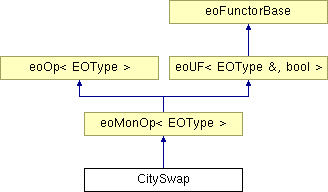
\includegraphics[height=4cm]{classCitySwap}
\end{center}
\end{figure}
\subsection*{Public Member Functions}
\begin{CompactItemize}
\item 
\hypertarget{classCitySwap_7e6958b62048c89604cbf046b86bdf2d}{
bool \hyperlink{classCitySwap_7e6958b62048c89604cbf046b86bdf2d}{operator()} (\bf{Route} \&\_\-\_\-route)}
\label{classCitySwap_7e6958b62048c89604cbf046b86bdf2d}

\end{CompactItemize}


\subsection{Detailed Description}
Its swaps two vertices randomly choosen. 



Definition at line 46 of file city\_\-swap.h.

The documentation for this class was generated from the following files:\begin{CompactItemize}
\item 
city\_\-swap.h\item 
city\_\-swap.cpp\end{CompactItemize}

\hypertarget{classCommunicable}{
\section{Communicable Class Reference}
\label{classCommunicable}\index{Communicable@{Communicable}}
}
Inheritance diagram for Communicable::\begin{figure}[H]
\begin{center}
\leavevmode
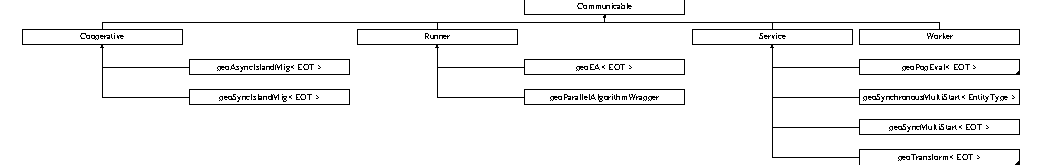
\includegraphics[height=2.22222cm]{classCommunicable}
\end{center}
\end{figure}
\subsection*{Public Member Functions}
\begin{CompactItemize}
\item 
\hypertarget{classCommunicable_8ae1827ecf7569b3db1ed386c7d8ad78}{
\hyperlink{classCommunicable_8ae1827ecf7569b3db1ed386c7d8ad78}{Communicable} ()}
\label{classCommunicable_8ae1827ecf7569b3db1ed386c7d8ad78}

\item 
\hypertarget{classCommunicable_2280b0dfa0d3a515fccf62c2a9fd5f41}{
virtual \hyperlink{classCommunicable_2280b0dfa0d3a515fccf62c2a9fd5f41}{$\sim$Communicable} ()}
\label{classCommunicable_2280b0dfa0d3a515fccf62c2a9fd5f41}

\item 
\hypertarget{classCommunicable_db4307b69b9ccacff55fdbf84b8f50e4}{
COMM\_\-ID \hyperlink{classCommunicable_db4307b69b9ccacff55fdbf84b8f50e4}{get\-Key} ()}
\label{classCommunicable_db4307b69b9ccacff55fdbf84b8f50e4}

\item 
\hypertarget{classCommunicable_e1f8bd1ee810fd73d44315c95998d19d}{
void \hyperlink{classCommunicable_e1f8bd1ee810fd73d44315c95998d19d}{lock} ()}
\label{classCommunicable_e1f8bd1ee810fd73d44315c95998d19d}

\item 
\hypertarget{classCommunicable_caa814847192e71f434fbf9479ede862}{
void \hyperlink{classCommunicable_caa814847192e71f434fbf9479ede862}{unlock} ()}
\label{classCommunicable_caa814847192e71f434fbf9479ede862}

\item 
\hypertarget{classCommunicable_cb53e6534b947bc889aa181d9dbbd13b}{
void \hyperlink{classCommunicable_cb53e6534b947bc889aa181d9dbbd13b}{stop} ()}
\label{classCommunicable_cb53e6534b947bc889aa181d9dbbd13b}

\item 
\hypertarget{classCommunicable_3306a9adb11a0ab5af342c0db9f7bb2a}{
void \hyperlink{classCommunicable_3306a9adb11a0ab5af342c0db9f7bb2a}{resume} ()}
\label{classCommunicable_3306a9adb11a0ab5af342c0db9f7bb2a}

\end{CompactItemize}
\subsection*{Protected Attributes}
\begin{CompactItemize}
\item 
\hypertarget{classCommunicable_605b0efeffe81326f216c9903f5bbf4c}{
COMM\_\-ID \hyperlink{classCommunicable_605b0efeffe81326f216c9903f5bbf4c}{key}}
\label{classCommunicable_605b0efeffe81326f216c9903f5bbf4c}

\item 
\hypertarget{classCommunicable_cf9639312f71a2f348bc1e7789ccbd9d}{
sem\_\-t \hyperlink{classCommunicable_cf9639312f71a2f348bc1e7789ccbd9d}{sem\_\-lock}}
\label{classCommunicable_cf9639312f71a2f348bc1e7789ccbd9d}

\item 
\hypertarget{classCommunicable_29c53b9191348e0505e3bcba6d8b82b1}{
sem\_\-t \hyperlink{classCommunicable_29c53b9191348e0505e3bcba6d8b82b1}{sem\_\-stop}}
\label{classCommunicable_29c53b9191348e0505e3bcba6d8b82b1}

\end{CompactItemize}
\subsection*{Static Protected Attributes}
\begin{CompactItemize}
\item 
\hypertarget{classCommunicable_7a6acfdc781a67c9c0ec4f17893f86c3}{
static unsigned \hyperlink{classCommunicable_7a6acfdc781a67c9c0ec4f17893f86c3}{num\_\-comm} = 0}
\label{classCommunicable_7a6acfdc781a67c9c0ec4f17893f86c3}

\end{CompactItemize}


\subsection{Detailed Description}




Definition at line 44 of file communicable.h.

The documentation for this class was generated from the following files:\begin{CompactItemize}
\item 
communicable.h\item 
communicable.cpp\end{CompactItemize}

\hypertarget{classCommunicator}{
\section{Communicator Class Reference}
\label{classCommunicator}\index{Communicator@{Communicator}}
}
Inheritance diagram for Communicator::\begin{figure}[H]
\begin{center}
\leavevmode
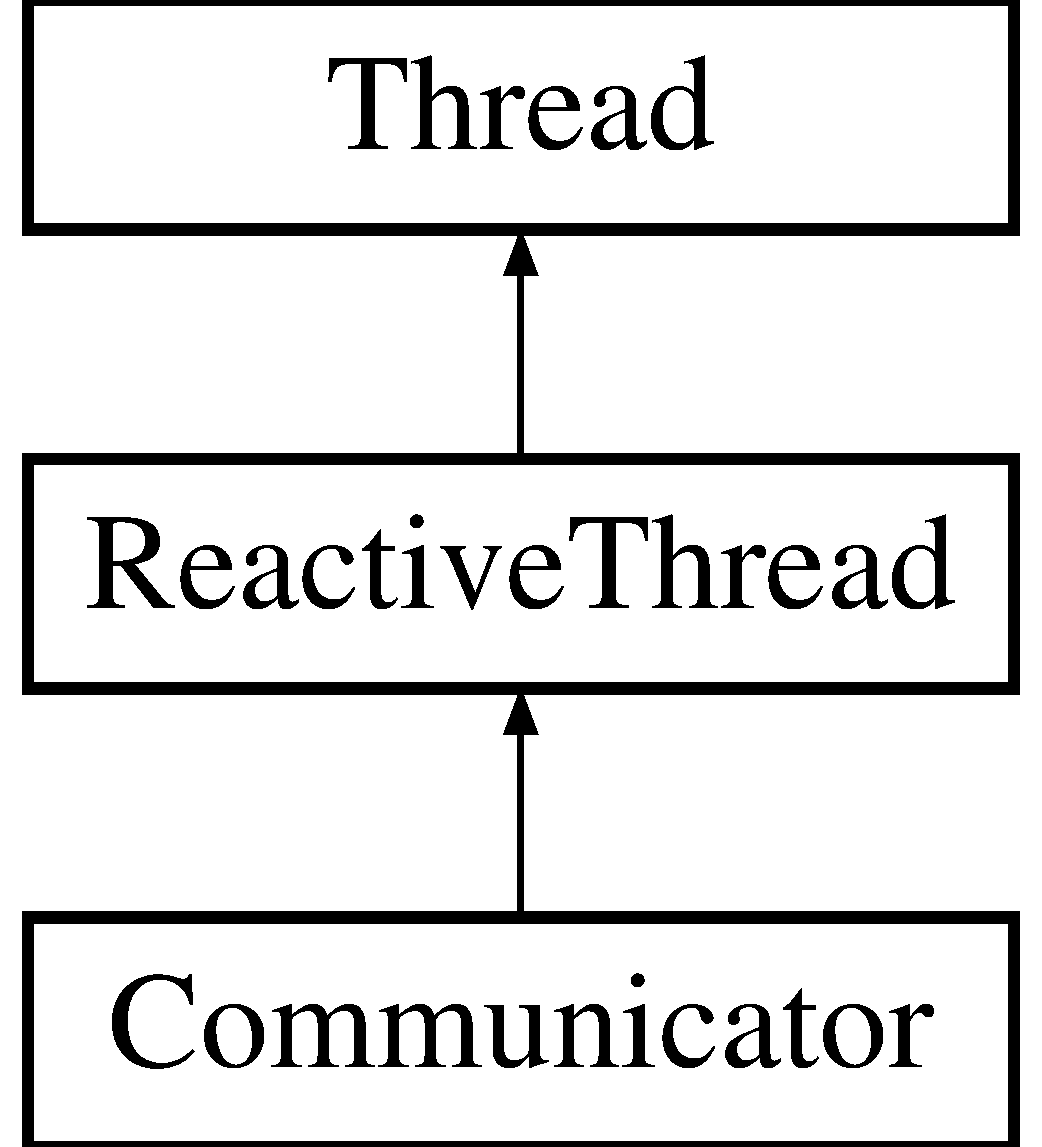
\includegraphics[height=3cm]{classCommunicator}
\end{center}
\end{figure}
\subsection*{Public Member Functions}
\begin{CompactItemize}
\item 
\hypertarget{classCommunicator_7c9dce4ea92bd04d01d53f80c0ef08ee}{
\hyperlink{classCommunicator_7c9dce4ea92bd04d01d53f80c0ef08ee}{Communicator} (int $\ast$\_\-\_\-argc, char $\ast$$\ast$$\ast$\_\-\_\-argv)}
\label{classCommunicator_7c9dce4ea92bd04d01d53f80c0ef08ee}

\item 
\hypertarget{classCommunicator_142fae13b16b166519315f248a513c62}{
void \hyperlink{classCommunicator_142fae13b16b166519315f248a513c62}{start} ()}
\label{classCommunicator_142fae13b16b166519315f248a513c62}

\end{CompactItemize}


\subsection{Detailed Description}




Definition at line 30 of file comm.h.

The documentation for this class was generated from the following files:\begin{CompactItemize}
\item 
comm.h\item 
comm.cpp\end{CompactItemize}

\hypertarget{classCompleteTopology}{
\section{Complete\-Topology Class Reference}
\label{classCompleteTopology}\index{CompleteTopology@{CompleteTopology}}
}
Inheritance diagram for Complete\-Topology::\begin{figure}[H]
\begin{center}
\leavevmode
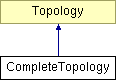
\includegraphics[height=2cm]{classCompleteTopology}
\end{center}
\end{figure}
\subsection*{Public Member Functions}
\begin{CompactItemize}
\item 
\hypertarget{classCompleteTopology_9ccbb45bf0cc00aff89fa8594746338c}{
void \hyperlink{classCompleteTopology_9ccbb45bf0cc00aff89fa8594746338c}{set\-Neighbors} (\hyperlink{classCooperative}{Cooperative} $\ast$\_\-\_\-mig, std::vector$<$ \hyperlink{classCooperative}{Cooperative} $\ast$ $>$ \&\_\-\_\-from, std::vector$<$ \hyperlink{classCooperative}{Cooperative} $\ast$ $>$ \&\_\-\_\-to)}
\label{classCompleteTopology_9ccbb45bf0cc00aff89fa8594746338c}

\end{CompactItemize}


\subsection{Detailed Description}




Definition at line 42 of file complete\_\-topo.h.

The documentation for this class was generated from the following files:\begin{CompactItemize}
\item 
complete\_\-topo.h\item 
complete\_\-topo.cpp\end{CompactItemize}

\hypertarget{classcontinuator}{
\section{continuator Class Reference}
\label{classcontinuator}\index{continuator@{continuator}}
}
Abstract class for a continuator within the exchange of data by migration.  


{\tt \#include $<$peo\-Data.h$>$}

Inheritance diagram for continuator::\begin{figure}[H]
\begin{center}
\leavevmode
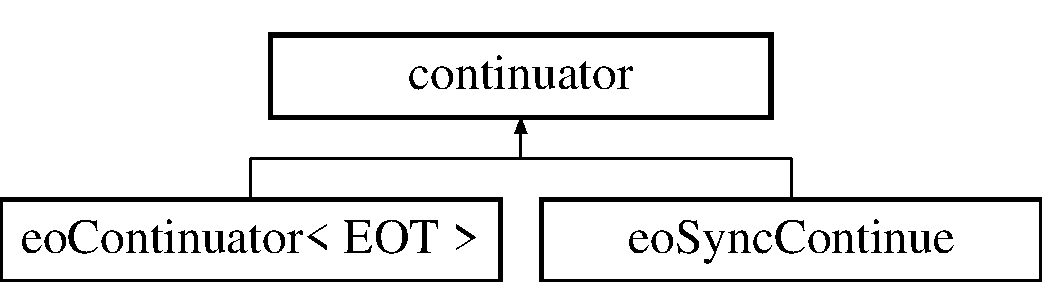
\includegraphics[height=2cm]{classcontinuator}
\end{center}
\end{figure}
\subsection*{Public Member Functions}
\begin{CompactItemize}
\item 
virtual bool \hyperlink{classcontinuator_30601b037ab27b40610af1b979ec3d5b}{check} ()=0
\begin{CompactList}\small\item\em Virtual function of check. \item\end{CompactList}\item 
\hypertarget{classcontinuator_bb29ad98fb4a158a5582c24873bf3f30}{
virtual \hyperlink{classcontinuator_bb29ad98fb4a158a5582c24873bf3f30}{$\sim$continuator} ()}
\label{classcontinuator_bb29ad98fb4a158a5582c24873bf3f30}

\begin{CompactList}\small\item\em Virtual destructor. \item\end{CompactList}\end{CompactItemize}


\subsection{Detailed Description}
Abstract class for a continuator within the exchange of data by migration. 

\begin{Desc}
\item[Version:]1.0 \end{Desc}
\begin{Desc}
\item[Date:]january 2008 \end{Desc}




Definition at line 51 of file peo\-Data.h.

\subsection{Member Function Documentation}
\hypertarget{classcontinuator_30601b037ab27b40610af1b979ec3d5b}{
\index{continuator@{continuator}!check@{check}}
\index{check@{check}!continuator@{continuator}}
\subsubsection[check]{\setlength{\rightskip}{0pt plus 5cm}virtual bool continuator::check ()\hspace{0.3cm}{\tt  \mbox{[}pure virtual\mbox{]}}}}
\label{classcontinuator_30601b037ab27b40610af1b979ec3d5b}


Virtual function of check. 

\begin{Desc}
\item[Returns:]true if the algorithm must continue \end{Desc}


Implemented in \hyperlink{classeoContinuator_4e599bd4db85a57b44f9b94580eee178}{eo\-Continuator$<$ EOT $>$}, and \hyperlink{classeoSyncContinue_417078233f768debb14b5a90f6412b3c}{eo\-Sync\-Continue}.

Referenced by peo\-Async\-Island\-Mig$<$ TYPESELECT, TYPEREPLACE $>$::operator()().

The documentation for this class was generated from the following file:\begin{CompactItemize}
\item 
peo\-Data.h\end{CompactItemize}

\hypertarget{classCooperative}{
\section{Cooperative Class Reference}
\label{classCooperative}\index{Cooperative@{Cooperative}}
}
Inheritance diagram for Cooperative::\begin{figure}[H]
\begin{center}
\leavevmode
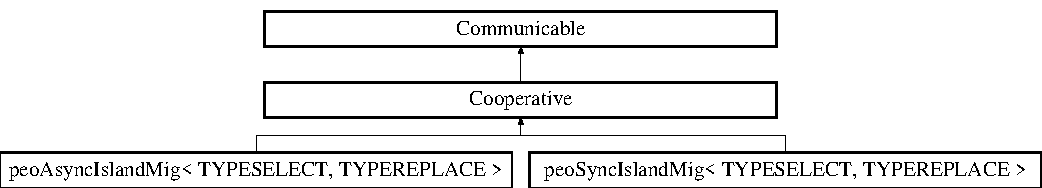
\includegraphics[height=2.53012cm]{classCooperative}
\end{center}
\end{figure}
\subsection*{Public Member Functions}
\begin{CompactItemize}
\item 
\hypertarget{classCooperative_4012b4e8329e87d26ee266491e1a883e}{
\hyperlink{classRunner}{Runner} $\ast$ \hyperlink{classCooperative_4012b4e8329e87d26ee266491e1a883e}{get\-Owner} ()}
\label{classCooperative_4012b4e8329e87d26ee266491e1a883e}

\item 
\hypertarget{classCooperative_fe7b022567174c8305bc78d8c5749b12}{
void \hyperlink{classCooperative_fe7b022567174c8305bc78d8c5749b12}{set\-Owner} (\hyperlink{classRunner}{Runner} \&\_\-\_\-runner)}
\label{classCooperative_fe7b022567174c8305bc78d8c5749b12}

\item 
\hypertarget{classCooperative_c609f2a1200da7d1ac96005602515fc6}{
void \hyperlink{classCooperative_c609f2a1200da7d1ac96005602515fc6}{send} (\hyperlink{classCooperative}{Cooperative} $\ast$\_\-\_\-coop)}
\label{classCooperative_c609f2a1200da7d1ac96005602515fc6}

\item 
\hypertarget{classCooperative_a08615f1fb5a71bb6eb8ea53ef7d1c69}{
void \hyperlink{classCooperative_a08615f1fb5a71bb6eb8ea53ef7d1c69}{synchronize\-Coop\-Ex} ()}
\label{classCooperative_a08615f1fb5a71bb6eb8ea53ef7d1c69}

\item 
\hypertarget{classCooperative_4439ddeaa1246a2e44c003bfb781739b}{
virtual void \hyperlink{classCooperative_4439ddeaa1246a2e44c003bfb781739b}{notify\-Sending} ()}
\label{classCooperative_4439ddeaa1246a2e44c003bfb781739b}

\item 
\hypertarget{classCooperative_b75a33c5735799076e01b125e47e3bbc}{
virtual void \hyperlink{classCooperative_b75a33c5735799076e01b125e47e3bbc}{notify\-Receiving} ()}
\label{classCooperative_b75a33c5735799076e01b125e47e3bbc}

\item 
\hypertarget{classCooperative_38f28f9155deac5e48edcaf935a2263b}{
virtual void \hyperlink{classCooperative_38f28f9155deac5e48edcaf935a2263b}{notify\-Sending\-Sync\-Req} ()}
\label{classCooperative_38f28f9155deac5e48edcaf935a2263b}

\item 
\hypertarget{classCooperative_6cc64e571944783b8f697f7c2299cc8d}{
virtual void \hyperlink{classCooperative_6cc64e571944783b8f697f7c2299cc8d}{notify\-Synchronized} ()}
\label{classCooperative_6cc64e571944783b8f697f7c2299cc8d}

\end{CompactItemize}
\subsection*{Private Attributes}
\begin{CompactItemize}
\item 
\hypertarget{classCooperative_7604f094479d08154ede4996a45bf79e}{
\hyperlink{classRunner}{Runner} $\ast$ \hyperlink{classCooperative_7604f094479d08154ede4996a45bf79e}{owner}}
\label{classCooperative_7604f094479d08154ede4996a45bf79e}

\end{CompactItemize}


\subsection{Detailed Description}




Definition at line 46 of file cooperative.h.

The documentation for this class was generated from the following files:\begin{CompactItemize}
\item 
cooperative.h\item 
cooperative.cpp\end{CompactItemize}

\hypertarget{classDisplayBestRoute}{
\section{Display\-Best\-Route Class Reference}
\label{classDisplayBestRoute}\index{DisplayBestRoute@{DisplayBestRoute}}
}
\subsection*{Public Member Functions}
\begin{CompactItemize}
\item 
\hypertarget{classDisplayBestRoute_db263e38f1e82174f811bf62f323f87f}{
\hyperlink{classDisplayBestRoute_db263e38f1e82174f811bf62f323f87f}{Display\-Best\-Route} (eo\-Pop$<$ Route $>$ \&\_\-\_\-pop)}
\label{classDisplayBestRoute_db263e38f1e82174f811bf62f323f87f}

\item 
\hypertarget{classDisplayBestRoute_ee879344a6d8b81a04d4eabbed2c7a04}{
void \hyperlink{classDisplayBestRoute_ee879344a6d8b81a04d4eabbed2c7a04}{operator()} ()}
\label{classDisplayBestRoute_ee879344a6d8b81a04d4eabbed2c7a04}

\end{CompactItemize}
\subsection*{Private Attributes}
\begin{CompactItemize}
\item 
\hypertarget{classDisplayBestRoute_5270aabbf294d2deca9878934216eb89}{
eo\-Pop$<$ Route $>$ \& \hyperlink{classDisplayBestRoute_5270aabbf294d2deca9878934216eb89}{pop}}
\label{classDisplayBestRoute_5270aabbf294d2deca9878934216eb89}

\end{CompactItemize}


\subsection{Detailed Description}




Definition at line 18 of file display\_\-best\_\-route.h.

The documentation for this class was generated from the following files:\begin{CompactItemize}
\item 
display\_\-best\_\-route.h\item 
display\_\-best\_\-route.cpp\end{CompactItemize}

\hypertarget{classEdgeXover}{
\section{Edge\-Xover Class Reference}
\label{classEdgeXover}\index{EdgeXover@{EdgeXover}}
}
Edge Crossover.  


{\tt \#include $<$edge\_\-xover.h$>$}

Inheritance diagram for Edge\-Xover::\begin{figure}[H]
\begin{center}
\leavevmode
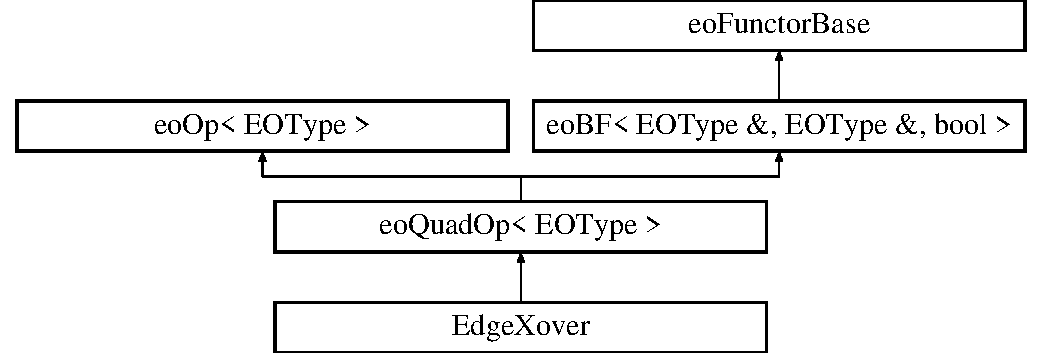
\includegraphics[height=4cm]{classEdgeXover}
\end{center}
\end{figure}
\subsection*{Public Member Functions}
\begin{CompactItemize}
\item 
\hypertarget{classEdgeXover_cb1c0a103106a4d3319540cb23163a79}{
bool \hyperlink{classEdgeXover_cb1c0a103106a4d3319540cb23163a79}{operator()} (\bf{Route} \&\_\-\_\-route1, \bf{Route} \&\_\-\_\-route2)}
\label{classEdgeXover_cb1c0a103106a4d3319540cb23163a79}

\end{CompactItemize}
\subsection*{Private Member Functions}
\begin{CompactItemize}
\item 
\hypertarget{classEdgeXover_88c2d4c9a878454a32d56010f3dddc27}{
void \hyperlink{classEdgeXover_88c2d4c9a878454a32d56010f3dddc27}{cross} (const \bf{Route} \&\_\-\_\-par1, const \bf{Route} \&\_\-\_\-par2, \bf{Route} \&\_\-\_\-child)}
\label{classEdgeXover_88c2d4c9a878454a32d56010f3dddc27}

\item 
\hypertarget{classEdgeXover_1b3a4c75dd9a034c81af6d89d85d30f5}{
void \hyperlink{classEdgeXover_1b3a4c75dd9a034c81af6d89d85d30f5}{remove\_\-entry} (unsigned \_\-\_\-vertex, std::vector$<$ std::set$<$ unsigned $>$ $>$ \&\_\-\_\-map)}
\label{classEdgeXover_1b3a4c75dd9a034c81af6d89d85d30f5}

\item 
\hypertarget{classEdgeXover_04de96aa1016836e0ba5f4b952a5fa16}{
void \hyperlink{classEdgeXover_04de96aa1016836e0ba5f4b952a5fa16}{build\_\-map} (const \bf{Route} \&\_\-\_\-par1, const \bf{Route} \&\_\-\_\-par2)}
\label{classEdgeXover_04de96aa1016836e0ba5f4b952a5fa16}

\item 
\hypertarget{classEdgeXover_2d3045ef503d8b16a27e11fdc23ca11c}{
void \hyperlink{classEdgeXover_2d3045ef503d8b16a27e11fdc23ca11c}{add\_\-vertex} (unsigned \_\-\_\-vertex, \bf{Route} \&\_\-\_\-child)}
\label{classEdgeXover_2d3045ef503d8b16a27e11fdc23ca11c}

\end{CompactItemize}
\subsection*{Private Attributes}
\begin{CompactItemize}
\item 
\hypertarget{classEdgeXover_d41399c6effb54ee48c722f1e19cb3c3}{
std::vector$<$ std::set$<$ unsigned $>$ $>$ \hyperlink{classEdgeXover_d41399c6effb54ee48c722f1e19cb3c3}{\_\-map}}
\label{classEdgeXover_d41399c6effb54ee48c722f1e19cb3c3}

\item 
\hypertarget{classEdgeXover_46d4d4724cf6d660b1a7ab4a346573d4}{
std::vector$<$ bool $>$ \hyperlink{classEdgeXover_46d4d4724cf6d660b1a7ab4a346573d4}{visited}}
\label{classEdgeXover_46d4d4724cf6d660b1a7ab4a346573d4}

\end{CompactItemize}


\subsection{Detailed Description}
Edge Crossover. 



Definition at line 48 of file edge\_\-xover.h.

The documentation for this class was generated from the following files:\begin{CompactItemize}
\item 
edge\_\-xover.h\item 
edge\_\-xover.cpp\end{CompactItemize}

\hypertarget{classeoContinuator}{
\section{eo\-Continuator$<$ EOT $>$ Class Template Reference}
\label{classeoContinuator}\index{eoContinuator@{eoContinuator}}
}
Specific class for a continuator within the exchange of migration of a population.  


{\tt \#include $<$peo\-Data.h$>$}

Inheritance diagram for eo\-Continuator$<$ EOT $>$::\begin{figure}[H]
\begin{center}
\leavevmode
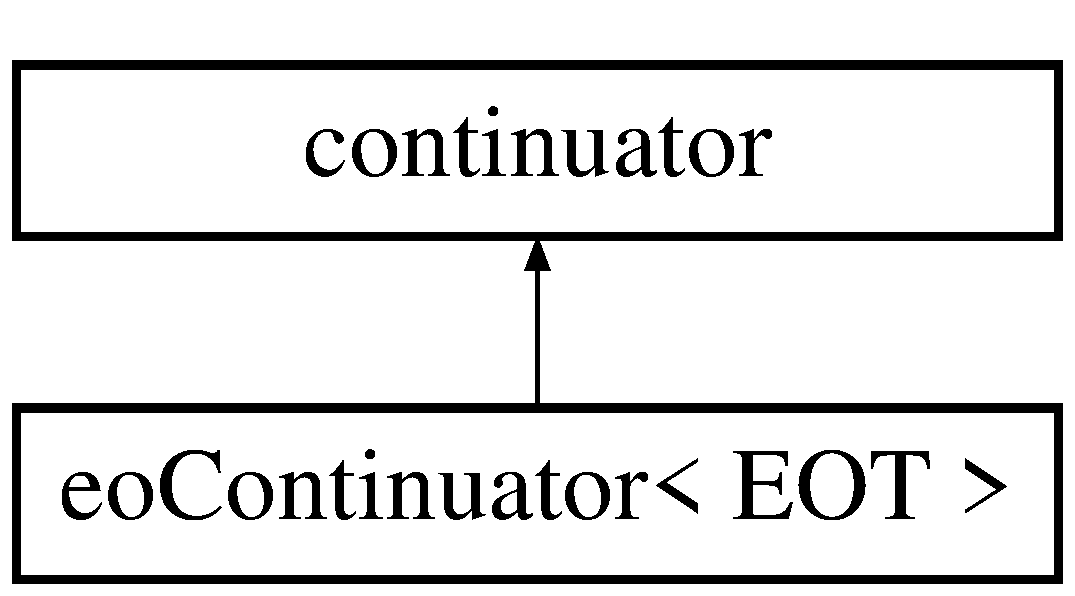
\includegraphics[height=2cm]{classeoContinuator}
\end{center}
\end{figure}
\subsection*{Public Member Functions}
\begin{CompactItemize}
\item 
\hyperlink{classeoContinuator_771e03f6ba647b2777dca2b8792fd317}{eo\-Continuator} (\bf{eo\-Continue}$<$ EOT $>$ \&\_\-cont, const \bf{eo\-Pop}$<$ EOT $>$ \&\_\-pop)
\begin{CompactList}\small\item\em Constructor. \item\end{CompactList}\item 
virtual bool \hyperlink{classeoContinuator_4e599bd4db85a57b44f9b94580eee178}{check} ()
\begin{CompactList}\small\item\em Virtual function of check. \item\end{CompactList}\end{CompactItemize}
\subsection*{Protected Attributes}
\begin{CompactItemize}
\item 
\bf{eo\-Continue}$<$ EOT $>$ \& \hyperlink{classeoContinuator_1c388d11915be8883f98a2511d598537}{cont}
\item 
\hypertarget{classeoContinuator_c10e809355df7bb763e4006ca02eab6c}{
const \bf{eo\-Pop}$<$ EOT $>$ \& \hyperlink{classeoContinuator_c10e809355df7bb763e4006ca02eab6c}{pop}}
\label{classeoContinuator_c10e809355df7bb763e4006ca02eab6c}

\end{CompactItemize}


\subsection{Detailed Description}
\subsubsection*{template$<$class EOT$>$ class eo\-Continuator$<$ EOT $>$}

Specific class for a continuator within the exchange of migration of a population. 

\begin{Desc}
\item[See also:]\hyperlink{classcontinuator}{continuator} \end{Desc}
\begin{Desc}
\item[Version:]1.0 \end{Desc}
\begin{Desc}
\item[Date:]january 2008 \end{Desc}




Definition at line 68 of file peo\-Data.h.

\subsection{Constructor \& Destructor Documentation}
\hypertarget{classeoContinuator_771e03f6ba647b2777dca2b8792fd317}{
\index{eoContinuator@{eo\-Continuator}!eoContinuator@{eoContinuator}}
\index{eoContinuator@{eoContinuator}!eoContinuator@{eo\-Continuator}}
\subsubsection[eoContinuator]{\setlength{\rightskip}{0pt plus 5cm}template$<$class EOT$>$ \hyperlink{classeoContinuator}{eo\-Continuator}$<$ EOT $>$::\hyperlink{classeoContinuator}{eo\-Continuator} (\bf{eo\-Continue}$<$ EOT $>$ \& {\em \_\-cont}, const \bf{eo\-Pop}$<$ EOT $>$ \& {\em \_\-pop})\hspace{0.3cm}{\tt  \mbox{[}inline\mbox{]}}}}
\label{classeoContinuator_771e03f6ba647b2777dca2b8792fd317}


Constructor. 

\begin{Desc}
\item[Parameters:]
\begin{description}
\item[{\em eo\-Continue$<$EOT$>$}]\& \item[{\em eo\-Pop$<$EOT$>$}]\& \end{description}
\end{Desc}


Definition at line 75 of file peo\-Data.h.

\subsection{Member Function Documentation}
\hypertarget{classeoContinuator_4e599bd4db85a57b44f9b94580eee178}{
\index{eoContinuator@{eo\-Continuator}!check@{check}}
\index{check@{check}!eoContinuator@{eo\-Continuator}}
\subsubsection[check]{\setlength{\rightskip}{0pt plus 5cm}template$<$class EOT$>$ virtual bool \hyperlink{classeoContinuator}{eo\-Continuator}$<$ EOT $>$::check ()\hspace{0.3cm}{\tt  \mbox{[}inline, virtual\mbox{]}}}}
\label{classeoContinuator_4e599bd4db85a57b44f9b94580eee178}


Virtual function of check. 

\begin{Desc}
\item[Returns:]false if the algorithm must continue \end{Desc}


Implements \hyperlink{classcontinuator_30601b037ab27b40610af1b979ec3d5b}{continuator}.

Definition at line 80 of file peo\-Data.h.

References eo\-Continuator$<$ EOT $>$::cont, and eo\-Continuator$<$ EOT $>$::pop.

\subsection{Member Data Documentation}
\hypertarget{classeoContinuator_1c388d11915be8883f98a2511d598537}{
\index{eoContinuator@{eo\-Continuator}!cont@{cont}}
\index{cont@{cont}!eoContinuator@{eo\-Continuator}}
\subsubsection[cont]{\setlength{\rightskip}{0pt plus 5cm}template$<$class EOT$>$ \bf{eo\-Continue}$<$EOT$>$\& \hyperlink{classeoContinuator}{eo\-Continuator}$<$ EOT $>$::\hyperlink{classeoContinuator_1c388d11915be8883f98a2511d598537}{cont}\hspace{0.3cm}{\tt  \mbox{[}protected\mbox{]}}}}
\label{classeoContinuator_1c388d11915be8883f98a2511d598537}


\begin{Desc}
\item[Parameters:]
\begin{description}
\item[{\em eo\-Continue$<$EOT$>$}]\& \item[{\em eo\-Pop$<$EOT$>$}]\& \end{description}
\end{Desc}


Definition at line 88 of file peo\-Data.h.

Referenced by eo\-Continuator$<$ EOT $>$::check().

The documentation for this class was generated from the following file:\begin{CompactItemize}
\item 
peo\-Data.h\end{CompactItemize}

\hypertarget{classeoReplace}{
\section{eo\-Replace$<$ EOT, TYPE $>$ Class Template Reference}
\label{classeoReplace}\index{eoReplace@{eoReplace}}
}
Specific class for a replacement within the exchange of migration of a population.  


{\tt \#include $<$peo\-Data.h$>$}

Inheritance diagram for eo\-Replace$<$ EOT, TYPE $>$::\begin{figure}[H]
\begin{center}
\leavevmode
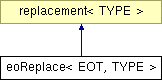
\includegraphics[height=2cm]{classeoReplace}
\end{center}
\end{figure}
\subsection*{Public Member Functions}
\begin{CompactItemize}
\item 
\hyperlink{classeoReplace_816081d8c7e8342d254402c5185efcbb}{eo\-Replace} (\bf{eo\-Replacement}$<$ EOT $>$ \&\_\-replace, TYPE \&\_\-destination)
\begin{CompactList}\small\item\em Constructor. \item\end{CompactList}\item 
virtual void \hyperlink{classeoReplace_786659edbd9907000138aa29caf46065}{operator()} (TYPE \&\_\-source)
\begin{CompactList}\small\item\em Virtual operator on the template type. \item\end{CompactList}\end{CompactItemize}
\subsection*{Protected Attributes}
\begin{CompactItemize}
\item 
\bf{eo\-Replacement}$<$ EOT $>$ \& \hyperlink{classeoReplace_b324e455db7f97021b0b7224a804b3e9}{replace}
\item 
\hypertarget{classeoReplace_9a0ec5ee11dfdd6f8077db89436cd5f8}{
TYPE \& \hyperlink{classeoReplace_9a0ec5ee11dfdd6f8077db89436cd5f8}{destination}}
\label{classeoReplace_9a0ec5ee11dfdd6f8077db89436cd5f8}

\end{CompactItemize}


\subsection{Detailed Description}
\subsubsection*{template$<$class EOT, class TYPE$>$ class eo\-Replace$<$ EOT, TYPE $>$}

Specific class for a replacement within the exchange of migration of a population. 

\begin{Desc}
\item[See also:]\hyperlink{classreplacement}{replacement} \end{Desc}
\begin{Desc}
\item[Version:]1.0 \end{Desc}
\begin{Desc}
\item[Date:]january 2008 \end{Desc}




Definition at line 173 of file peo\-Data.h.

\subsection{Constructor \& Destructor Documentation}
\hypertarget{classeoReplace_816081d8c7e8342d254402c5185efcbb}{
\index{eoReplace@{eo\-Replace}!eoReplace@{eoReplace}}
\index{eoReplace@{eoReplace}!eoReplace@{eo\-Replace}}
\subsubsection[eoReplace]{\setlength{\rightskip}{0pt plus 5cm}template$<$class EOT, class TYPE$>$ \hyperlink{classeoReplace}{eo\-Replace}$<$ EOT, TYPE $>$::\hyperlink{classeoReplace}{eo\-Replace} (\bf{eo\-Replacement}$<$ EOT $>$ \& {\em \_\-replace}, TYPE \& {\em \_\-destination})\hspace{0.3cm}{\tt  \mbox{[}inline\mbox{]}}}}
\label{classeoReplace_816081d8c7e8342d254402c5185efcbb}


Constructor. 

\begin{Desc}
\item[Parameters:]
\begin{description}
\item[{\em eo\-Replacement$<$EOT$>$}]\& \item[{\em TYPE}]\& \_\-destination (with TYPE which is the template type) \end{description}
\end{Desc}


Definition at line 179 of file peo\-Data.h.

\subsection{Member Function Documentation}
\hypertarget{classeoReplace_786659edbd9907000138aa29caf46065}{
\index{eoReplace@{eo\-Replace}!operator()@{operator()}}
\index{operator()@{operator()}!eoReplace@{eo\-Replace}}
\subsubsection[operator()]{\setlength{\rightskip}{0pt plus 5cm}template$<$class EOT, class TYPE$>$ virtual void \hyperlink{classeoReplace}{eo\-Replace}$<$ EOT, TYPE $>$::operator() (TYPE \& {\em \_\-source})\hspace{0.3cm}{\tt  \mbox{[}inline, virtual\mbox{]}}}}
\label{classeoReplace_786659edbd9907000138aa29caf46065}


Virtual operator on the template type. 

\begin{Desc}
\item[Parameters:]
\begin{description}
\item[{\em TYPE}]\& \_\-source \end{description}
\end{Desc}


Implements \hyperlink{classreplacement_2c21feaad602bb9d691f0081ac4363b1}{replacement$<$ TYPE $>$}.

Definition at line 184 of file peo\-Data.h.

References eo\-Replace$<$ EOT, TYPE $>$::destination, and eo\-Replace$<$ EOT, TYPE $>$::replace.

\subsection{Member Data Documentation}
\hypertarget{classeoReplace_b324e455db7f97021b0b7224a804b3e9}{
\index{eoReplace@{eo\-Replace}!replace@{replace}}
\index{replace@{replace}!eoReplace@{eo\-Replace}}
\subsubsection[replace]{\setlength{\rightskip}{0pt plus 5cm}template$<$class EOT, class TYPE$>$ \bf{eo\-Replacement}$<$EOT$>$\& \hyperlink{classeoReplace}{eo\-Replace}$<$ EOT, TYPE $>$::\hyperlink{classeoReplace_b324e455db7f97021b0b7224a804b3e9}{replace}\hspace{0.3cm}{\tt  \mbox{[}protected\mbox{]}}}}
\label{classeoReplace_b324e455db7f97021b0b7224a804b3e9}


\begin{Desc}
\item[Parameters:]
\begin{description}
\item[{\em eo\-Replacement$<$EOT$>$}]\& \item[{\em TYPE}]\& destination \end{description}
\end{Desc}


Definition at line 192 of file peo\-Data.h.

Referenced by eo\-Replace$<$ EOT, TYPE $>$::operator()().

The documentation for this class was generated from the following file:\begin{CompactItemize}
\item 
peo\-Data.h\end{CompactItemize}

\hypertarget{classeoSelector}{
\section{eo\-Selector$<$ EOT, TYPE $>$ Class Template Reference}
\label{classeoSelector}\index{eoSelector@{eoSelector}}
}
Specific class for a selector within the exchange of migration of a population.  


{\tt \#include $<$peo\-Data.h$>$}

Inheritance diagram for eo\-Selector$<$ EOT, TYPE $>$::\begin{figure}[H]
\begin{center}
\leavevmode
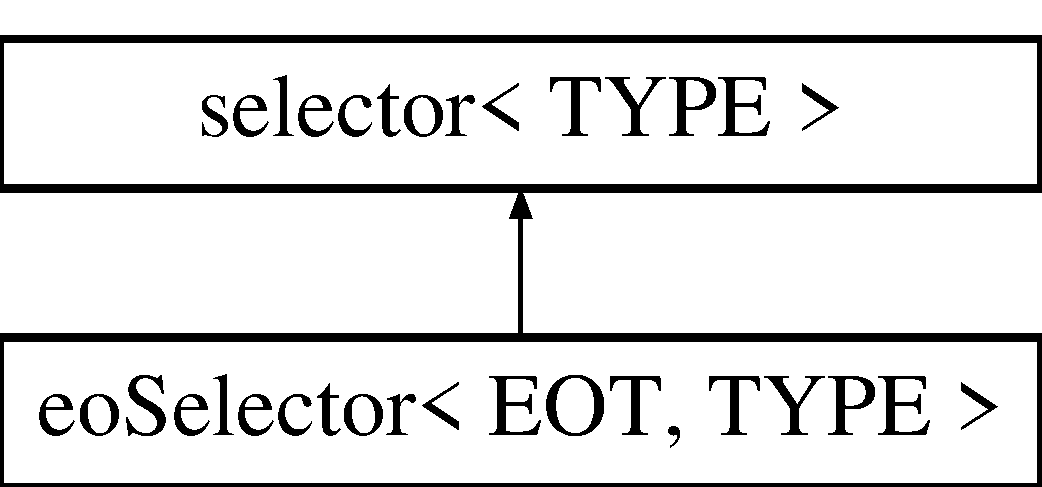
\includegraphics[height=2cm]{classeoSelector}
\end{center}
\end{figure}
\subsection*{Public Member Functions}
\begin{CompactItemize}
\item 
\hyperlink{classeoSelector_29942b726f94d10091e056c9f3076f27}{eo\-Selector} (\bf{eo\-Select\-One}$<$ EOT $>$ \&\_\-select, unsigned \_\-nb\_\-select, const TYPE \&\_\-source)
\begin{CompactList}\small\item\em Constructor. \item\end{CompactList}\item 
virtual void \hyperlink{classeoSelector_2f32b10e23e68654e4459bb682aaa4ff}{operator()} (TYPE \&\_\-dest)
\begin{CompactList}\small\item\em Virtual operator on the template type. \item\end{CompactList}\end{CompactItemize}
\subsection*{Protected Attributes}
\begin{CompactItemize}
\item 
\bf{eo\-Select\-One}$<$ EOT $>$ \& \hyperlink{classeoSelector_b44e120fc689d7775135ad576b2c66e9}{selector}
\item 
\hypertarget{classeoSelector_285c6b6f0bd0e0e173468009369a391e}{
unsigned \hyperlink{classeoSelector_285c6b6f0bd0e0e173468009369a391e}{nb\_\-select}}
\label{classeoSelector_285c6b6f0bd0e0e173468009369a391e}

\item 
\hypertarget{classeoSelector_7cf15424f32a7ef6f534babca5a24236}{
const TYPE \& \hyperlink{classeoSelector_7cf15424f32a7ef6f534babca5a24236}{source}}
\label{classeoSelector_7cf15424f32a7ef6f534babca5a24236}

\end{CompactItemize}


\subsection{Detailed Description}
\subsubsection*{template$<$class EOT, class TYPE$>$ class eo\-Selector$<$ EOT, TYPE $>$}

Specific class for a selector within the exchange of migration of a population. 

\begin{Desc}
\item[See also:]\hyperlink{classselector}{selector} \end{Desc}
\begin{Desc}
\item[Version:]1.0 \end{Desc}
\begin{Desc}
\item[Date:]january 2008 \end{Desc}




Definition at line 118 of file peo\-Data.h.

\subsection{Constructor \& Destructor Documentation}
\hypertarget{classeoSelector_29942b726f94d10091e056c9f3076f27}{
\index{eoSelector@{eo\-Selector}!eoSelector@{eoSelector}}
\index{eoSelector@{eoSelector}!eoSelector@{eo\-Selector}}
\subsubsection[eoSelector]{\setlength{\rightskip}{0pt plus 5cm}template$<$class EOT, class TYPE$>$ \hyperlink{classeoSelector}{eo\-Selector}$<$ EOT, TYPE $>$::\hyperlink{classeoSelector}{eo\-Selector} (\bf{eo\-Select\-One}$<$ EOT $>$ \& {\em \_\-select}, unsigned {\em \_\-nb\_\-select}, const TYPE \& {\em \_\-source})\hspace{0.3cm}{\tt  \mbox{[}inline\mbox{]}}}}
\label{classeoSelector_29942b726f94d10091e056c9f3076f27}


Constructor. 

\begin{Desc}
\item[Parameters:]
\begin{description}
\item[{\em \doxyref{eo\-Select\-One$<$EOT$>$}}]\& \item[{\em unsigned}]\_\-nb\_\-select \item[{\em TYPE}]\& \_\-source (with TYPE which is the template type) \end{description}
\end{Desc}


Definition at line 126 of file peo\-Data.h.

\subsection{Member Function Documentation}
\hypertarget{classeoSelector_2f32b10e23e68654e4459bb682aaa4ff}{
\index{eoSelector@{eo\-Selector}!operator()@{operator()}}
\index{operator()@{operator()}!eoSelector@{eo\-Selector}}
\subsubsection[operator()]{\setlength{\rightskip}{0pt plus 5cm}template$<$class EOT, class TYPE$>$ virtual void \hyperlink{classeoSelector}{eo\-Selector}$<$ EOT, TYPE $>$::operator() (TYPE \& {\em \_\-dest})\hspace{0.3cm}{\tt  \mbox{[}inline, virtual\mbox{]}}}}
\label{classeoSelector_2f32b10e23e68654e4459bb682aaa4ff}


Virtual operator on the template type. 

\begin{Desc}
\item[Parameters:]
\begin{description}
\item[{\em TYPE}]\& \_\-dest \end{description}
\end{Desc}


Implements \hyperlink{classselector_3ca409d57262f397263541753c7fcc28}{selector$<$ TYPE $>$}.

Definition at line 131 of file peo\-Data.h.

References eo\-Selector$<$ EOT, TYPE $>$::nb\_\-select, eo\-Selector$<$ EOT, TYPE $>$::selector, and eo\-Selector$<$ EOT, TYPE $>$::source.

\subsection{Member Data Documentation}
\hypertarget{classeoSelector_b44e120fc689d7775135ad576b2c66e9}{
\index{eoSelector@{eo\-Selector}!selector@{selector}}
\index{selector@{selector}!eoSelector@{eo\-Selector}}
\subsubsection[selector]{\setlength{\rightskip}{0pt plus 5cm}template$<$class EOT, class TYPE$>$ \bf{eo\-Select\-One}$<$EOT$>$\& \hyperlink{classeoSelector}{eo\-Selector}$<$ EOT, TYPE $>$::\hyperlink{classselector}{selector}\hspace{0.3cm}{\tt  \mbox{[}protected\mbox{]}}}}
\label{classeoSelector_b44e120fc689d7775135ad576b2c66e9}


\begin{Desc}
\item[Parameters:]
\begin{description}
\item[{\em \doxyref{eo\-Select\-One$<$EOT$>$}}]\& \item[{\em unsigned}]nb\_\-select \item[{\em TYPE}]\& source \end{description}
\end{Desc}


Definition at line 143 of file peo\-Data.h.

Referenced by eo\-Selector$<$ EOT, TYPE $>$::operator()().

The documentation for this class was generated from the following file:\begin{CompactItemize}
\item 
peo\-Data.h\end{CompactItemize}

\hypertarget{classeoSyncContinue}{
\section{eo\-Sync\-Continue Class Reference}
\label{classeoSyncContinue}\index{eoSyncContinue@{eoSyncContinue}}
}
Class for a continuator within the exchange of data by synchrone migration.  


{\tt \#include $<$peo\-Data.h$>$}

Inheritance diagram for eo\-Sync\-Continue::\begin{figure}[H]
\begin{center}
\leavevmode
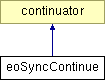
\includegraphics[height=2cm]{classeoSyncContinue}
\end{center}
\end{figure}
\subsection*{Public Member Functions}
\begin{CompactItemize}
\item 
\hyperlink{classeoSyncContinue_a1f0cb0e380ffffd964031c4aa0f7086}{eo\-Sync\-Continue} (unsigned \_\-\_\-period, unsigned \_\-\_\-init\_\-counter=0)
\begin{CompactList}\small\item\em Constructor. \item\end{CompactList}\item 
virtual bool \hyperlink{classeoSyncContinue_417078233f768debb14b5a90f6412b3c}{check} ()
\begin{CompactList}\small\item\em Virtual function of check. \item\end{CompactList}\end{CompactItemize}
\subsection*{Private Attributes}
\begin{CompactItemize}
\item 
unsigned \hyperlink{classeoSyncContinue_966a94a44db2f84c7df0ef3d4694e37c}{period}
\item 
\hypertarget{classeoSyncContinue_c2e6e2b929884e370b16f2cccda9cd17}{
unsigned \hyperlink{classeoSyncContinue_c2e6e2b929884e370b16f2cccda9cd17}{counter}}
\label{classeoSyncContinue_c2e6e2b929884e370b16f2cccda9cd17}

\end{CompactItemize}


\subsection{Detailed Description}
Class for a continuator within the exchange of data by synchrone migration. 

\begin{Desc}
\item[See also:]\hyperlink{classcontinuator}{continuator} \end{Desc}
\begin{Desc}
\item[Version:]1.0 \end{Desc}
\begin{Desc}
\item[Date:]january 2008 \end{Desc}




Definition at line 206 of file peo\-Data.h.

\subsection{Constructor \& Destructor Documentation}
\hypertarget{classeoSyncContinue_a1f0cb0e380ffffd964031c4aa0f7086}{
\index{eoSyncContinue@{eo\-Sync\-Continue}!eoSyncContinue@{eoSyncContinue}}
\index{eoSyncContinue@{eoSyncContinue}!eoSyncContinue@{eo\-Sync\-Continue}}
\subsubsection[eoSyncContinue]{\setlength{\rightskip}{0pt plus 5cm}eo\-Sync\-Continue::eo\-Sync\-Continue (unsigned {\em \_\-\_\-period}, unsigned {\em \_\-\_\-init\_\-counter} = {\tt 0})\hspace{0.3cm}{\tt  \mbox{[}inline\mbox{]}}}}
\label{classeoSyncContinue_a1f0cb0e380ffffd964031c4aa0f7086}


Constructor. 

\begin{Desc}
\item[Parameters:]
\begin{description}
\item[{\em unsigned}]\_\-\_\-period \item[{\em unsigned}]\_\-\_\-init\_\-counter \end{description}
\end{Desc}


Definition at line 213 of file peo\-Data.h.

\subsection{Member Function Documentation}
\hypertarget{classeoSyncContinue_417078233f768debb14b5a90f6412b3c}{
\index{eoSyncContinue@{eo\-Sync\-Continue}!check@{check}}
\index{check@{check}!eoSyncContinue@{eo\-Sync\-Continue}}
\subsubsection[check]{\setlength{\rightskip}{0pt plus 5cm}virtual bool eo\-Sync\-Continue::check ()\hspace{0.3cm}{\tt  \mbox{[}inline, virtual\mbox{]}}}}
\label{classeoSyncContinue_417078233f768debb14b5a90f6412b3c}


Virtual function of check. 

\begin{Desc}
\item[Returns:]true if the algorithm must continue \end{Desc}


Implements \hyperlink{classcontinuator_30601b037ab27b40610af1b979ec3d5b}{continuator}.

Definition at line 218 of file peo\-Data.h.

References counter, and period.

Referenced by peo\-Sync\-Island\-Mig$<$ TYPESELECT, TYPEREPLACE $>$::operator()().

\subsection{Member Data Documentation}
\hypertarget{classeoSyncContinue_966a94a44db2f84c7df0ef3d4694e37c}{
\index{eoSyncContinue@{eo\-Sync\-Continue}!period@{period}}
\index{period@{period}!eoSyncContinue@{eo\-Sync\-Continue}}
\subsubsection[period]{\setlength{\rightskip}{0pt plus 5cm}unsigned \hyperlink{classeoSyncContinue_966a94a44db2f84c7df0ef3d4694e37c}{eo\-Sync\-Continue::period}\hspace{0.3cm}{\tt  \mbox{[}private\mbox{]}}}}
\label{classeoSyncContinue_966a94a44db2f84c7df0ef3d4694e37c}


\begin{Desc}
\item[Parameters:]
\begin{description}
\item[{\em unsigned}]period \item[{\em unsigned}]counter \end{description}
\end{Desc}


Definition at line 227 of file peo\-Data.h.

Referenced by check().

The documentation for this class was generated from the following file:\begin{CompactItemize}
\item 
peo\-Data.h\end{CompactItemize}

\hypertarget{classMergeRouteEval}{
\section{Merge\-Route\-Eval Class Reference}
\label{classMergeRouteEval}\index{MergeRouteEval@{MergeRouteEval}}
}
Inheritance diagram for Merge\-Route\-Eval::\begin{figure}[H]
\begin{center}
\leavevmode
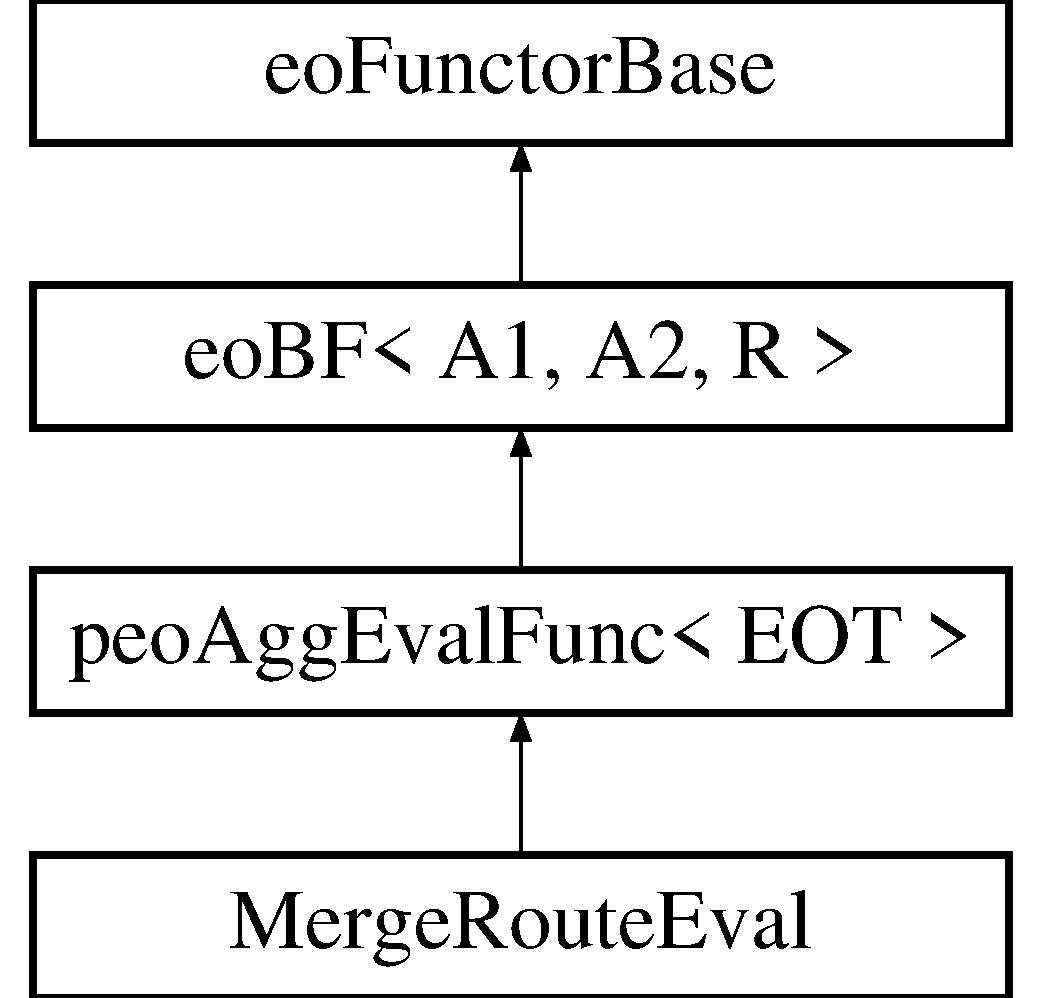
\includegraphics[height=2cm]{classMergeRouteEval}
\end{center}
\end{figure}
\subsection*{Public Member Functions}
\begin{CompactItemize}
\item 
\hypertarget{classMergeRouteEval_29cb0028ac0df4b2cee3a809c8f35dea}{
void \hyperlink{classMergeRouteEval_29cb0028ac0df4b2cee3a809c8f35dea}{operator()} (Route \&\_\-\_\-route, const int \&\_\-\_\-part\_\-fit)}
\label{classMergeRouteEval_29cb0028ac0df4b2cee3a809c8f35dea}

\end{CompactItemize}


\subsection{Detailed Description}




Definition at line 31 of file merge\_\-route\_\-eval.h.

The documentation for this class was generated from the following files:\begin{CompactItemize}
\item 
merge\_\-route\_\-eval.h\item 
merge\_\-route\_\-eval.cpp\end{CompactItemize}

\hypertarget{classMPIThreadedEnv}{
\section{MPIThreaded\-Env Class Reference}
\label{classMPIThreadedEnv}\index{MPIThreadedEnv@{MPIThreadedEnv}}
}
\subsection*{Static Public Member Functions}
\begin{CompactItemize}
\item 
\hypertarget{classMPIThreadedEnv_ce2a77c94cd4304117d8241e97050b96}{
static void \hyperlink{classMPIThreadedEnv_ce2a77c94cd4304117d8241e97050b96}{init} (int $\ast$\_\-\_\-argc, char $\ast$$\ast$$\ast$\_\-\_\-argv)}
\label{classMPIThreadedEnv_ce2a77c94cd4304117d8241e97050b96}

\item 
\hypertarget{classMPIThreadedEnv_6be33c401734f7359724895c1c21ecd2}{
static void \hyperlink{classMPIThreadedEnv_6be33c401734f7359724895c1c21ecd2}{finalize} ()}
\label{classMPIThreadedEnv_6be33c401734f7359724895c1c21ecd2}

\end{CompactItemize}
\subsection*{Private Member Functions}
\begin{CompactItemize}
\item 
\hypertarget{classMPIThreadedEnv_b499d64e6e095f4bfebd91604d0d6d5c}{
\hyperlink{classMPIThreadedEnv_b499d64e6e095f4bfebd91604d0d6d5c}{MPIThreaded\-Env} (int $\ast$\_\-\_\-argc, char $\ast$$\ast$$\ast$\_\-\_\-argv)}
\label{classMPIThreadedEnv_b499d64e6e095f4bfebd91604d0d6d5c}

\item 
\hypertarget{classMPIThreadedEnv_9fc0c3ae7f4599d34cdb3a541f7b24fa}{
\hyperlink{classMPIThreadedEnv_9fc0c3ae7f4599d34cdb3a541f7b24fa}{$\sim$MPIThreaded\-Env} ()}
\label{classMPIThreadedEnv_9fc0c3ae7f4599d34cdb3a541f7b24fa}

\end{CompactItemize}


\subsection{Detailed Description}




Definition at line 46 of file src/rmc/mpi/node.cpp.

The documentation for this class was generated from the following file:\begin{CompactItemize}
\item 
src/rmc/mpi/node.cpp\end{CompactItemize}

\hypertarget{classOrderXover}{
\section{Order\-Xover Class Reference}
\label{classOrderXover}\index{OrderXover@{OrderXover}}
}
Order Crossover.  


{\tt \#include $<$order\_\-xover.h$>$}

\subsection*{Public Member Functions}
\begin{CompactItemize}
\item 
\hypertarget{classOrderXover_0ff6aada669eb8173322ed68cda1ac61}{
bool \hyperlink{classOrderXover_0ff6aada669eb8173322ed68cda1ac61}{operator()} (Route \&\_\-\_\-route1, Route \&\_\-\_\-route2)}
\label{classOrderXover_0ff6aada669eb8173322ed68cda1ac61}

\end{CompactItemize}
\subsection*{Private Member Functions}
\begin{CompactItemize}
\item 
\hypertarget{classOrderXover_d2bf90b5f46ac4a344777e17bc5f364d}{
void \hyperlink{classOrderXover_d2bf90b5f46ac4a344777e17bc5f364d}{cross} (const Route \&\_\-\_\-par1, const Route \&\_\-\_\-par2, Route \&\_\-\_\-child)}
\label{classOrderXover_d2bf90b5f46ac4a344777e17bc5f364d}

\end{CompactItemize}


\subsection{Detailed Description}
Order Crossover. 



Definition at line 17 of file order\_\-xover.h.

The documentation for this class was generated from the following files:\begin{CompactItemize}
\item 
order\_\-xover.h\item 
order\_\-xover.cpp\end{CompactItemize}

\hypertarget{classPartialMappedXover}{
\section{Partial\-Mapped\-Xover Class Reference}
\label{classPartialMappedXover}\index{PartialMappedXover@{PartialMappedXover}}
}
Partial Mapped Crossover.  


{\tt \#include $<$partial\_\-mapped\_\-xover.h$>$}

\subsection*{Public Member Functions}
\begin{CompactItemize}
\item 
\hypertarget{classPartialMappedXover_1cda6ea86ca36e5de0125f4ba5cfc695}{
bool \hyperlink{classPartialMappedXover_1cda6ea86ca36e5de0125f4ba5cfc695}{operator()} (Route \&\_\-\_\-route1, Route \&\_\-\_\-route2)}
\label{classPartialMappedXover_1cda6ea86ca36e5de0125f4ba5cfc695}

\end{CompactItemize}
\subsection*{Private Member Functions}
\begin{CompactItemize}
\item 
\hypertarget{classPartialMappedXover_b6d4035544aff3b2b3fe4b0eeea185a2}{
void \hyperlink{classPartialMappedXover_b6d4035544aff3b2b3fe4b0eeea185a2}{repair} (Route \&\_\-\_\-route, unsigned \_\-\_\-cut1, unsigned \_\-\_\-cut2)}
\label{classPartialMappedXover_b6d4035544aff3b2b3fe4b0eeea185a2}

\end{CompactItemize}


\subsection{Detailed Description}
Partial Mapped Crossover. 



Definition at line 32 of file partial\_\-mapped\_\-xover.h.

The documentation for this class was generated from the following files:\begin{CompactItemize}
\item 
partial\_\-mapped\_\-xover.h\item 
partial\_\-mapped\_\-xover.cpp\end{CompactItemize}

\hypertarget{classPartRouteEval}{
\section{Part\-Route\-Eval Class Reference}
\label{classPartRouteEval}\index{PartRouteEval@{PartRouteEval}}
}
Route Evaluator.  


{\tt \#include $<$part\_\-route\_\-eval.h$>$}

Inheritance diagram for Part\-Route\-Eval::\begin{figure}[H]
\begin{center}
\leavevmode
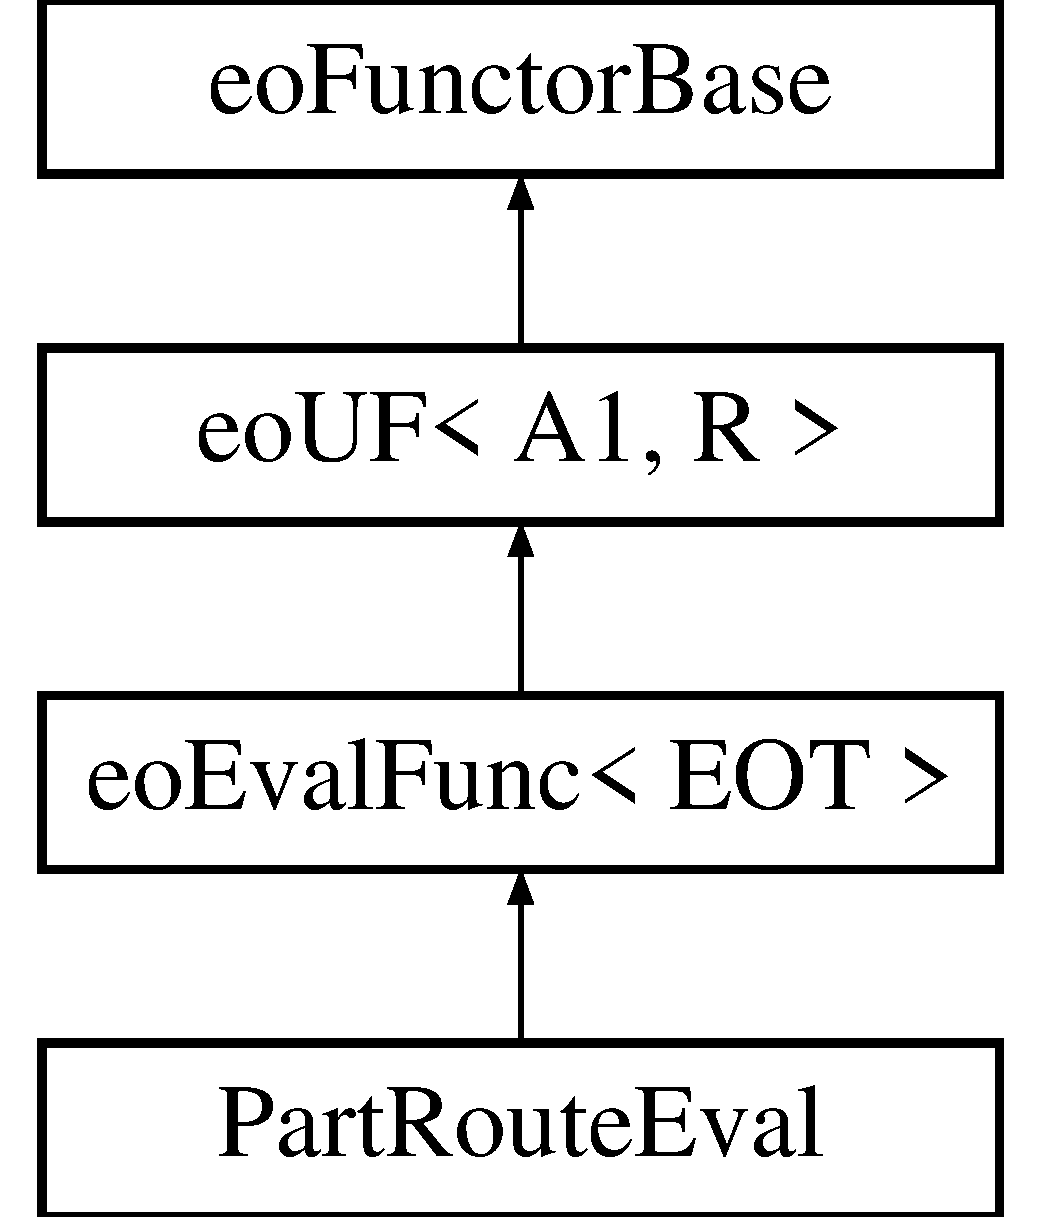
\includegraphics[height=4cm]{classPartRouteEval}
\end{center}
\end{figure}
\subsection*{Public Member Functions}
\begin{CompactItemize}
\item 
\hypertarget{classPartRouteEval_a331566b29bc3227f377004232f05491}{
\hyperlink{classPartRouteEval_a331566b29bc3227f377004232f05491}{Part\-Route\-Eval} (float \_\-\_\-from, float \_\-\_\-to)}
\label{classPartRouteEval_a331566b29bc3227f377004232f05491}

\begin{CompactList}\small\item\em Constructor. \item\end{CompactList}\item 
\hypertarget{classPartRouteEval_965fab875fb601f17934a6ece761beae}{
void \hyperlink{classPartRouteEval_965fab875fb601f17934a6ece761beae}{operator()} (\bf{Route} \&\_\-\_\-route)}
\label{classPartRouteEval_965fab875fb601f17934a6ece761beae}

\end{CompactItemize}
\subsection*{Private Attributes}
\begin{CompactItemize}
\item 
\hypertarget{classPartRouteEval_5bde722e66378b2570ae6c4b4f8df58e}{
float \hyperlink{classPartRouteEval_5bde722e66378b2570ae6c4b4f8df58e}{from}}
\label{classPartRouteEval_5bde722e66378b2570ae6c4b4f8df58e}

\item 
\hypertarget{classPartRouteEval_de53cc919faa498663f327b72c357da3}{
float \hyperlink{classPartRouteEval_de53cc919faa498663f327b72c357da3}{to}}
\label{classPartRouteEval_de53cc919faa498663f327b72c357da3}

\end{CompactItemize}


\subsection{Detailed Description}
Route Evaluator. 



Definition at line 45 of file part\_\-route\_\-eval.h.

The documentation for this class was generated from the following files:\begin{CompactItemize}
\item 
part\_\-route\_\-eval.h\item 
part\_\-route\_\-eval.cpp\end{CompactItemize}

\hypertarget{classpeoAggEvalFunc}{
\section{peo\-Agg\-Eval\-Func$<$ EOT $>$ Class Template Reference}
\label{classpeoAggEvalFunc}\index{peoAggEvalFunc@{peoAggEvalFunc}}
}
The \hyperlink{classpeoAggEvalFunc}{peo\-Agg\-Eval\-Func} class offers only the interface for creating aggregate evaluation functions - there are no direct internal functions provided.  


{\tt \#include $<$peo\-Agg\-Eval\-Func.h$>$}

Inheritance diagram for peo\-Agg\-Eval\-Func$<$ EOT $>$::\begin{figure}[H]
\begin{center}
\leavevmode
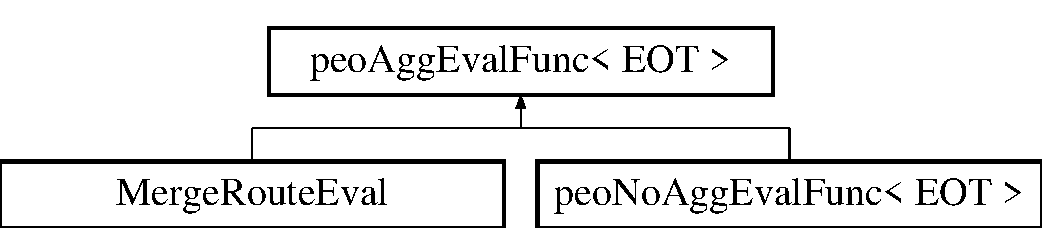
\includegraphics[height=2cm]{classpeoAggEvalFunc}
\end{center}
\end{figure}


\subsection{Detailed Description}
\subsubsection*{template$<$class EOT$>$ class peo\-Agg\-Eval\-Func$<$ EOT $>$}

The \hyperlink{classpeoAggEvalFunc}{peo\-Agg\-Eval\-Func} class offers only the interface for creating aggregate evaluation functions - there are no direct internal functions provided. 

The class inherits {\bf public eo\-BF$<$ EOT\&, const typename EOT :: Fitness\&, void $>$} thus requiring, for the derived classes, the creation of a function having the following signature:

\begin{TabularC}{2}
\hline
void operator()( EOT\& \_\-\_\-eot, const typename EOT :: Fitness\& \_\-\_\-partial\_\-fittness ); ~ &~  \\\hline
\end{TabularC}


The aggregation object is called in an iterative manner for each of the results obtained by applying partial evaluation functions. 



Definition at line 25 of file peo\-Agg\-Eval\-Func.h.

The documentation for this class was generated from the following file:\begin{CompactItemize}
\item 
peo\-Agg\-Eval\-Func.h\end{CompactItemize}

\hypertarget{classpeoAsyncIslandMig}{
\section{peo\-Async\-Island\-Mig$<$ EOT $>$ Class Template Reference}
\label{classpeoAsyncIslandMig}\index{peoAsyncIslandMig@{peoAsyncIslandMig}}
}
The \hyperlink{classpeoAsyncIslandMig}{peo\-Async\-Island\-Mig} class offers the elementary basis for implementating an asynchronous island migration model - requires the specification of several basic parameters, i.e.  


{\tt \#include $<$peo\-Async\-Island\-Mig.h$>$}

Inheritance diagram for peo\-Async\-Island\-Mig$<$ EOT $>$::\begin{figure}[H]
\begin{center}
\leavevmode
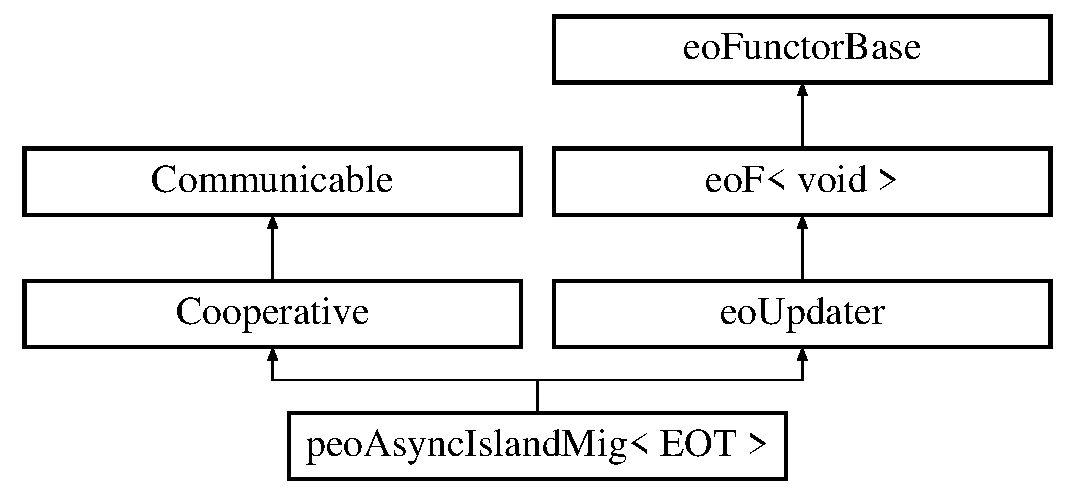
\includegraphics[height=3cm]{classpeoAsyncIslandMig}
\end{center}
\end{figure}
\subsection*{Public Member Functions}
\begin{CompactItemize}
\item 
\hyperlink{classpeoAsyncIslandMig_e0f706cbf4148d3ca327227a5c7a9fdf}{peo\-Async\-Island\-Mig} (eo\-Continue$<$ EOT $>$ \&\_\-\_\-cont, eo\-Select$<$ EOT $>$ \&\_\-\_\-select, eo\-Replacement$<$ EOT $>$ \&\_\-\_\-replace, \hyperlink{classTopology}{Topology} \&\_\-\_\-topology, eo\-Pop$<$ EOT $>$ \&\_\-\_\-source, eo\-Pop$<$ EOT $>$ \&\_\-\_\-destination)
\begin{CompactList}\small\item\em Constructor for the \hyperlink{classpeoAsyncIslandMig}{peo\-Async\-Island\-Mig} class; the characteristics of the migration model are defined through the specified parameters - out of the box objects provided in EO, etc., or custom, derived objects may be passed as parameters. \item\end{CompactList}\item 
void \hyperlink{classpeoAsyncIslandMig_13581e54425727a7f785ca8a6df527b5}{operator()} ()
\begin{CompactList}\small\item\em Function operator to be called as checkpoint for performing the migration step. \item\end{CompactList}\item 
\hypertarget{classpeoAsyncIslandMig_6d790a5d0b6ac510cac4f61a1c0d8f16}{
void \hyperlink{classpeoAsyncIslandMig_6d790a5d0b6ac510cac4f61a1c0d8f16}{pack} ()}
\label{classpeoAsyncIslandMig_6d790a5d0b6ac510cac4f61a1c0d8f16}

\begin{CompactList}\small\item\em Auxiliary function dealing with sending the emigrant individuals. There is no need to explicitly call the function. \item\end{CompactList}\item 
\hypertarget{classpeoAsyncIslandMig_455501aee5db2bbfbae15779c8429369}{
void \hyperlink{classpeoAsyncIslandMig_455501aee5db2bbfbae15779c8429369}{unpack} ()}
\label{classpeoAsyncIslandMig_455501aee5db2bbfbae15779c8429369}

\begin{CompactList}\small\item\em Auxiliary function dealing with receiving immigrant individuals. There is no need to explicitly call the function. \item\end{CompactList}\end{CompactItemize}
\subsection*{Private Member Functions}
\begin{CompactItemize}
\item 
\hypertarget{classpeoAsyncIslandMig_87a4ef7d4bd30d349a801bf0f9e87c82}{
void \hyperlink{classpeoAsyncIslandMig_87a4ef7d4bd30d349a801bf0f9e87c82}{emigrate} ()}
\label{classpeoAsyncIslandMig_87a4ef7d4bd30d349a801bf0f9e87c82}

\item 
\hypertarget{classpeoAsyncIslandMig_5a9a64ba51a696e45f91b362c39c9a64}{
void \hyperlink{classpeoAsyncIslandMig_5a9a64ba51a696e45f91b362c39c9a64}{immigrate} ()}
\label{classpeoAsyncIslandMig_5a9a64ba51a696e45f91b362c39c9a64}

\end{CompactItemize}
\subsection*{Private Attributes}
\begin{CompactItemize}
\item 
\hypertarget{classpeoAsyncIslandMig_2fc077d02ef9ea4595cfe883af0d4f83}{
eo\-Continue$<$ EOT $>$ \& \hyperlink{classpeoAsyncIslandMig_2fc077d02ef9ea4595cfe883af0d4f83}{cont}}
\label{classpeoAsyncIslandMig_2fc077d02ef9ea4595cfe883af0d4f83}

\item 
\hypertarget{classpeoAsyncIslandMig_b1fa045094c8a411323e75b5820c80c2}{
eo\-Select$<$ EOT $>$ \& \hyperlink{classpeoAsyncIslandMig_b1fa045094c8a411323e75b5820c80c2}{select}}
\label{classpeoAsyncIslandMig_b1fa045094c8a411323e75b5820c80c2}

\item 
\hypertarget{classpeoAsyncIslandMig_b761dbd880ee32e170741ecd78da6f48}{
eo\-Replacement$<$ EOT $>$ \& \hyperlink{classpeoAsyncIslandMig_b761dbd880ee32e170741ecd78da6f48}{replace}}
\label{classpeoAsyncIslandMig_b761dbd880ee32e170741ecd78da6f48}

\item 
\hypertarget{classpeoAsyncIslandMig_e45e5a808a96f0853ab6ba42339fe679}{
\hyperlink{classTopology}{Topology} \& \hyperlink{classpeoAsyncIslandMig_e45e5a808a96f0853ab6ba42339fe679}{topology}}
\label{classpeoAsyncIslandMig_e45e5a808a96f0853ab6ba42339fe679}

\item 
\hypertarget{classpeoAsyncIslandMig_8a502d82c773033e274dca932fc2d4ee}{
eo\-Pop$<$ EOT $>$ \& \hyperlink{classpeoAsyncIslandMig_8a502d82c773033e274dca932fc2d4ee}{source}}
\label{classpeoAsyncIslandMig_8a502d82c773033e274dca932fc2d4ee}

\item 
\hypertarget{classpeoAsyncIslandMig_e407f411d08ae7d96992603c145a7e43}{
eo\-Pop$<$ EOT $>$ \& \hyperlink{classpeoAsyncIslandMig_e407f411d08ae7d96992603c145a7e43}{destination}}
\label{classpeoAsyncIslandMig_e407f411d08ae7d96992603c145a7e43}

\item 
\hypertarget{classpeoAsyncIslandMig_b8c76d98d9ae99dd930a77c12860519a}{
std::queue$<$ eo\-Pop$<$ EOT $>$ $>$ \hyperlink{classpeoAsyncIslandMig_b8c76d98d9ae99dd930a77c12860519a}{imm}}
\label{classpeoAsyncIslandMig_b8c76d98d9ae99dd930a77c12860519a}

\item 
\hypertarget{classpeoAsyncIslandMig_a9cc0e2d61cac6e11647b141962adc89}{
std::queue$<$ eo\-Pop$<$ EOT $>$ $>$ \hyperlink{classpeoAsyncIslandMig_a9cc0e2d61cac6e11647b141962adc89}{em}}
\label{classpeoAsyncIslandMig_a9cc0e2d61cac6e11647b141962adc89}

\item 
\hypertarget{classpeoAsyncIslandMig_1a2c0004d23bc303420af137a8c8bd27}{
std::queue$<$ \hyperlink{classCooperative}{Cooperative} $\ast$ $>$ \hyperlink{classpeoAsyncIslandMig_1a2c0004d23bc303420af137a8c8bd27}{coop\_\-em}}
\label{classpeoAsyncIslandMig_1a2c0004d23bc303420af137a8c8bd27}

\end{CompactItemize}


\subsection{Detailed Description}
\subsubsection*{template$<$class EOT$>$ class peo\-Async\-Island\-Mig$<$ EOT $>$}

The \hyperlink{classpeoAsyncIslandMig}{peo\-Async\-Island\-Mig} class offers the elementary basis for implementating an asynchronous island migration model - requires the specification of several basic parameters, i.e. 

continuation criterion, selection and replacement strategies, a topological model and the source and destination population for the migrating individuals. As opposed to the synchronous migration model, in the asynchronous migration approach, there is no synchronization step between islands after performing the emigration phase.

The migration operator is called at the end of each generation of an evolutionary algorithms as a checkpoint object - the following code exposes the structure of a classic evolutionary algorithm:

\begin{TabularC}{2}
\hline
{\bf do} \{ ~ &~  \\\hline
~~~~~~~~ select( population, offsprings ); ~ &// select the offsprings from the current population \\\hline
~~~~~~~~ transform( offsprings ); ~ &// crossover and mutation operators are applied on the selected offsprings \\\hline
~~~~~~~~ evaluate( offsprings ); ~ &// evaluation step of the resulting offsprings \\\hline
~~~~~~~~ replace( population, offsprings ); ~ &// replace the individuals in the current population whith individuals from the offspring population, according to a specified replacement strategy \\\hline
\} {\bf while} ( ea\-Checkpoint\-Continue( population ) ); ~ &// checkpoint operators are applied on the current population, including the migration operator, if any specified  \\\hline
\end{TabularC}


Constructing an asynchronous island migration model requires having defined (1) a topological migration model, (2) the control parameters of the migration process, (3) a checkpoint object associated with an evolutionary algorithm, and (4) an owner object must be set. The owner object must be derived from the {\bf \hyperlink{classRunner}{Runner}} class (for example a \hyperlink{classpeoEA}{peo\-EA} object represents a possible owner). A simple example is offered bellow:

\begin{enumerate}
\item topological model to be followed when performing migrations: \par
 \par
 \begin{TabularC}{2}
\hline
\hyperlink{classRingTopology}{Ring\-Topology} mig\-Topology; ~ &// a simple ring topological model - each island communicates with two other islands \\\hline
\end{TabularC}


\item the continuation criterion, selection and replacement strategy etc. are defined: \par
 \par
 \begin{TabularC}{2}
\hline
eo\-Pop$<$ EOT $>$ population( POP\_\-SIZE, pop\-Initializer ); ~ &// population of individuals to be used for the evolutionary algorithm \\\hline
~  &~  \\\hline
eo\-Periodic\-Continue$<$ EOT $>$ mig\-Cont( MIG\_\-FREQ ); ~ &// migrations occur periodically at MIG\_\-FREQ iterations \\\hline
eo\-Random\-Select$<$ EOT $>$ mig\-Select\-Strategy; ~ &// selection strategy - in this case a random selection is applied \\\hline
eo\-Select\-Number$<$ EOT $>$ mig\-Select( mig\-Select\-Strategy, MIG\_\-SIZE ); ~ &// number of individuals to be selected using the specified strategy \\\hline
eo\-Plus\-Replacement$<$ EOT $>$ mig\-Replace; ~ &// immigration strategy - the worse individuals in the destination population are replaced by the immigrant individuals \\\hline
~  &~  \\\hline
peo\-Async\-Island\-Mig$<$ EOT $>$ async\-Migration( \par
 ~~~~~~~~ mig\-Cont, mig\-Select, mig\-Replace, mig\-Topology, \par
 ~~~~~~~~ population, population \par
 ); ~  &// asynchronous migration object - the emigrant individuals are selected from the same from population in which the immigrant individuals are being integrated  \\\hline
\end{TabularC}


\item creation of a checkpoint object as part of the definition of an evolutionary algoritm (details of th EA not given as being out of scope): \par
 \par
 \begin{TabularC}{2}
\hline
... ~ &~  \\\hline
eo\-Gen\-Continue$<$ EOT $>$ ea\-Cont( NUM\_\-GEN ); ~ &// the evolutionary algorithm will stop after NUM\_\-GEN generations \\\hline
eo\-Check\-Point$<$ EOT $>$ ea\-Checkpoint\-Continue( ea\-Cont ); ~ &// number of individuals to be selected using the specified strategy \\\hline
... ~ &~  \\\hline
ea\-Checkpoint\-Continue.add( async\-Migration ); ~ &// adding the migration operator as checkpoint element \\\hline
... ~ &~  \\\hline
\end{TabularC}


\item definition of an owner evolutionary algorithm (an object inheriting the {\bf \hyperlink{classRunner}{Runner}} class): \par
 \par
 \begin{TabularC}{2}
\hline
peo\-EA$<$ EOT $>$ ea\-Alg( ea\-Checkpoint\-Continue, ea\-Pop\-Eval, ea\-Select, ea\-Transform, ea\-Replace); ~ &// evolutionary algorithm having as checkpoint the ea\-Checkpoint\-Continue object defined above  \\\hline
async\-Migration.set\-Owner( ea\-Alg ); ~ &// setting the evolutionary algorithm as owner of the migration object  \\\hline
ea\-Alg( population ); ~ &// applying the evolutionary algorithm on a given population  \\\hline
\end{TabularC}
\end{enumerate}


The source and the destination population for the migration object were specified as being the same, in step no. 2, as we are usually interested in selecting the emigrants and integrating the immigrant individuals from and in, respectively, one unique population, iteratively evolved by an evolutionary algorithm. There is no restriction in having two distinct populations as source and destination for the emigrant and immigrant individuals respectively.

The above steps only create an asynchronous migration object associated to an evolutionary algorithm. The creation of several islands requires the reiteration of the steps 2 through 4 for creating distinct algorithms, with distinct populations and the associated distinctly parametrized migration objects. The interconnecting element is the underlying topology, defined at step 1 (the same C++ mig\-Topology object has to be passed as parameter for all the migration objects, in order to interconnect them). 



Definition at line 112 of file peo\-Async\-Island\-Mig.h.

\subsection{Constructor \& Destructor Documentation}
\hypertarget{classpeoAsyncIslandMig_e0f706cbf4148d3ca327227a5c7a9fdf}{
\index{peoAsyncIslandMig@{peo\-Async\-Island\-Mig}!peoAsyncIslandMig@{peoAsyncIslandMig}}
\index{peoAsyncIslandMig@{peoAsyncIslandMig}!peoAsyncIslandMig@{peo\-Async\-Island\-Mig}}
\subsubsection[peoAsyncIslandMig]{\setlength{\rightskip}{0pt plus 5cm}template$<$class EOT$>$ \hyperlink{classpeoAsyncIslandMig}{peo\-Async\-Island\-Mig}$<$ EOT $>$::\hyperlink{classpeoAsyncIslandMig}{peo\-Async\-Island\-Mig} (eo\-Continue$<$ EOT $>$ \& {\em \_\-\_\-cont}, eo\-Select$<$ EOT $>$ \& {\em \_\-\_\-select}, eo\-Replacement$<$ EOT $>$ \& {\em \_\-\_\-replace}, \hyperlink{classTopology}{Topology} \& {\em \_\-\_\-topology}, eo\-Pop$<$ EOT $>$ \& {\em \_\-\_\-source}, eo\-Pop$<$ EOT $>$ \& {\em \_\-\_\-destination})}}
\label{classpeoAsyncIslandMig_e0f706cbf4148d3ca327227a5c7a9fdf}


Constructor for the \hyperlink{classpeoAsyncIslandMig}{peo\-Async\-Island\-Mig} class; the characteristics of the migration model are defined through the specified parameters - out of the box objects provided in EO, etc., or custom, derived objects may be passed as parameters. 

\begin{Desc}
\item[Parameters:]
\begin{description}
\item[{\em eo\-Continue$<$}]EOT $>$\& \_\-\_\-cont - continuation criterion specifying whether the migration is performed or not; \item[{\em eo\-Select$<$}]EOT $>$\& \_\-\_\-select - selection strategy to be applied for constructing a list of emigrant individuals out of the source population; \item[{\em eo\-Replacement$<$}]EOT $>$\& \_\-\_\-replace - replacement strategy used for integrating the immigrant individuals in the destination population; \item[{\em Topology\&}]\_\-\_\-topology - topological model to be followed when performing migrations; \item[{\em eo\-Pop$<$}]EOT $>$\& \_\-\_\-source - source population from which the emigrant individuals are selected; \item[{\em eo\-Pop$<$}]EOT $>$\& \_\-\_\-destination - destination population in which the immigrant population are integrated. \end{description}
\end{Desc}


Definition at line 171 of file peo\-Async\-Island\-Mig.h.

References Topology::add().

\subsection{Member Function Documentation}
\hypertarget{classpeoAsyncIslandMig_13581e54425727a7f785ca8a6df527b5}{
\index{peoAsyncIslandMig@{peo\-Async\-Island\-Mig}!operator()@{operator()}}
\index{operator()@{operator()}!peoAsyncIslandMig@{peo\-Async\-Island\-Mig}}
\subsubsection[operator()]{\setlength{\rightskip}{0pt plus 5cm}template$<$class EOT$>$ void \hyperlink{classpeoAsyncIslandMig}{peo\-Async\-Island\-Mig}$<$ EOT $>$::operator() ()}}
\label{classpeoAsyncIslandMig_13581e54425727a7f785ca8a6df527b5}


Function operator to be called as checkpoint for performing the migration step. 

The emigrant individuals are selected from the source population and sent to the next island (defined by the topology object) while the immigrant individuals are integrated in the destination population. There is no need to explicitly call the function - the wrapper checkpoint object (please refer to the above example) will perform the call when required. 

Definition at line 248 of file peo\-Async\-Island\-Mig.h.

References peo\-Async\-Island\-Mig$<$ EOT $>$::cont, peo\-Async\-Island\-Mig$<$ EOT $>$::emigrate(), peo\-Async\-Island\-Mig$<$ EOT $>$::immigrate(), and peo\-Async\-Island\-Mig$<$ EOT $>$::source.

The documentation for this class was generated from the following file:\begin{CompactItemize}
\item 
peo\-Async\-Island\-Mig.h\end{CompactItemize}

\hypertarget{structpeoEvalFunc}{
\section{peo\-Eval\-Func$<$ EOT, Fit\-T, Function\-Arg $>$ Class Template Reference}
\label{structpeoEvalFunc}\index{peoEvalFunc@{peoEvalFunc}}
}
Specific class for evaluation.  


{\tt \#include $<$peo\-Eval\-Func.h$>$}

Inheritance diagram for peo\-Eval\-Func$<$ EOT, Fit\-T, Function\-Arg $>$::\begin{figure}[H]
\begin{center}
\leavevmode
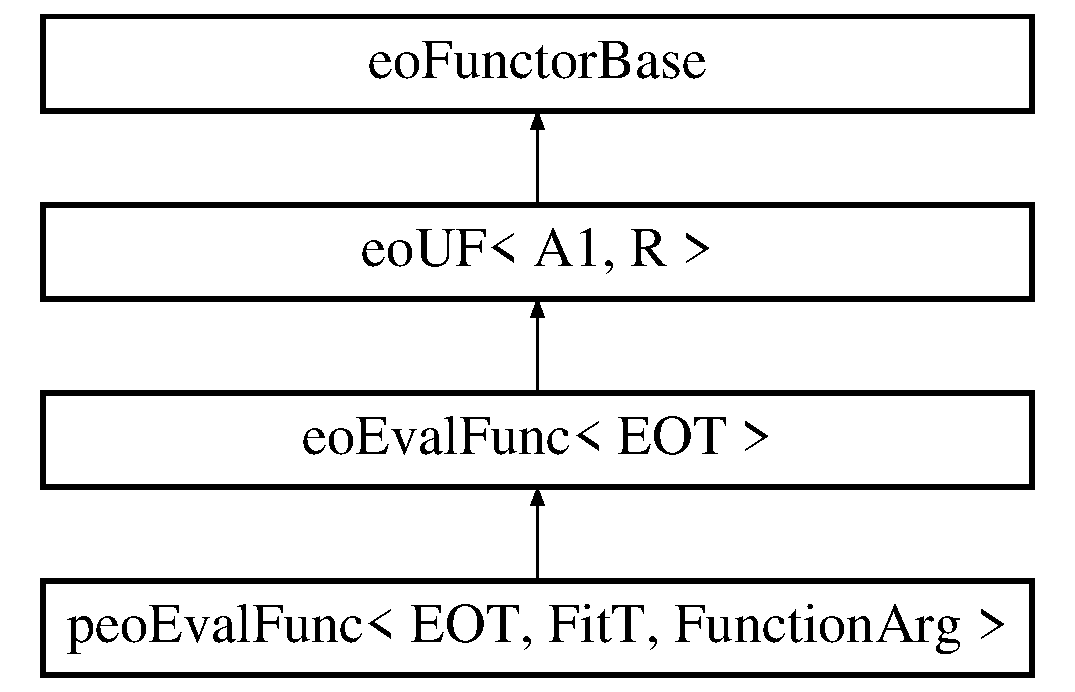
\includegraphics[height=4cm]{structpeoEvalFunc}
\end{center}
\end{figure}
\subsection*{Public Member Functions}
\begin{CompactItemize}
\item 
\hyperlink{structpeoEvalFunc_e4168d7266c801802fba855d019e6733}{peo\-Eval\-Func} (Fit\-T($\ast$\_\-eval)(Function\-Arg))
\begin{CompactList}\small\item\em Constructor. \item\end{CompactList}\item 
virtual void \hyperlink{structpeoEvalFunc_c9b1903cca26f12905a6e12d1753c7cd}{operator()} (EOT \&\_\-peo)
\begin{CompactList}\small\item\em Virtual operator. \item\end{CompactList}\end{CompactItemize}
\subsection*{Private Attributes}
\begin{CompactItemize}
\item 
Fit\-T($\ast$ \hyperlink{structpeoEvalFunc_aacd84e82536aa8ce1cb4d4cebaa691a}{eval\-Func} )(Function\-Arg)
\end{CompactItemize}


\subsection{Detailed Description}
\subsubsection*{template$<$class EOT, class Fit\-T = typename EOT::Fitness, class Function\-Arg = const EOT\&$>$ class peo\-Eval\-Func$<$ EOT, Fit\-T, Function\-Arg $>$}

Specific class for evaluation. 

\begin{Desc}
\item[See also:]\doxyref{eo\-Eval\-Func} \end{Desc}
\begin{Desc}
\item[Version:]1.0 \end{Desc}
\begin{Desc}
\item[Date:]november 2007 \end{Desc}




Definition at line 50 of file peo\-Eval\-Func.h.

\subsection{Constructor \& Destructor Documentation}
\hypertarget{structpeoEvalFunc_e4168d7266c801802fba855d019e6733}{
\index{peoEvalFunc@{peo\-Eval\-Func}!peoEvalFunc@{peoEvalFunc}}
\index{peoEvalFunc@{peoEvalFunc}!peoEvalFunc@{peo\-Eval\-Func}}
\subsubsection[peoEvalFunc]{\setlength{\rightskip}{0pt plus 5cm}template$<$class EOT, class Fit\-T = typename EOT::Fitness, class Function\-Arg = const EOT\&$>$ \hyperlink{structpeoEvalFunc}{peo\-Eval\-Func}$<$ EOT, Fit\-T, Function\-Arg $>$::\hyperlink{structpeoEvalFunc}{peo\-Eval\-Func} (Fit\-T($\ast$)(Function\-Arg) {\em \_\-eval})\hspace{0.3cm}{\tt  \mbox{[}inline\mbox{]}}}}
\label{structpeoEvalFunc_e4168d7266c801802fba855d019e6733}


Constructor. 

\begin{Desc}
\item[Parameters:]
\begin{description}
\item[{\em Fit\-T}]($\ast$ \_\-eval)( Function\-Arg ) \end{description}
\end{Desc}


Definition at line 55 of file peo\-Eval\-Func.h.

\subsection{Member Function Documentation}
\hypertarget{structpeoEvalFunc_c9b1903cca26f12905a6e12d1753c7cd}{
\index{peoEvalFunc@{peo\-Eval\-Func}!operator()@{operator()}}
\index{operator()@{operator()}!peoEvalFunc@{peo\-Eval\-Func}}
\subsubsection[operator()]{\setlength{\rightskip}{0pt plus 5cm}template$<$class EOT, class Fit\-T = typename EOT::Fitness, class Function\-Arg = const EOT\&$>$ virtual void \hyperlink{structpeoEvalFunc}{peo\-Eval\-Func}$<$ EOT, Fit\-T, Function\-Arg $>$::operator() (EOT \& {\em \_\-peo})\hspace{0.3cm}{\tt  \mbox{[}inline, virtual\mbox{]}}}}
\label{structpeoEvalFunc_c9b1903cca26f12905a6e12d1753c7cd}


Virtual operator. 

\begin{Desc}
\item[Parameters:]
\begin{description}
\item[{\em EOT}]\& \_\-peo \end{description}
\end{Desc}


Definition at line 61 of file peo\-Eval\-Func.h.

References peo\-Eval\-Func$<$ EOT, Fit\-T, Function\-Arg $>$::eval\-Func.

\subsection{Member Data Documentation}
\hypertarget{structpeoEvalFunc_aacd84e82536aa8ce1cb4d4cebaa691a}{
\index{peoEvalFunc@{peo\-Eval\-Func}!evalFunc@{evalFunc}}
\index{evalFunc@{evalFunc}!peoEvalFunc@{peo\-Eval\-Func}}
\subsubsection[evalFunc]{\setlength{\rightskip}{0pt plus 5cm}template$<$class EOT, class Fit\-T = typename EOT::Fitness, class Function\-Arg = const EOT\&$>$ Fit\-T($\ast$  \hyperlink{structpeoEvalFunc}{peo\-Eval\-Func}$<$ EOT, Fit\-T, Function\-Arg $>$::\hyperlink{structpeoEvalFunc_aacd84e82536aa8ce1cb4d4cebaa691a}{eval\-Func})(Function\-Arg)\hspace{0.3cm}{\tt  \mbox{[}private\mbox{]}}}}
\label{structpeoEvalFunc_aacd84e82536aa8ce1cb4d4cebaa691a}


\begin{Desc}
\item[Parameters:]
\begin{description}
\item[{\em Fit\-T}]($\ast$ eval\-Func )( Function\-Arg ) \end{description}
\end{Desc}


Referenced by peo\-Eval\-Func$<$ EOT, Fit\-T, Function\-Arg $>$::operator()().

The documentation for this class was generated from the following file:\begin{CompactItemize}
\item 
peo\-Eval\-Func.h\end{CompactItemize}

\hypertarget{classpeoGlobalBestVelocity}{
\section{peo\-Global\-Best\-Velocity$<$ POT $>$ Class Template Reference}
\label{classpeoGlobalBestVelocity}\index{peoGlobalBestVelocity@{peoGlobalBestVelocity}}
}
Specific class for a replacement thanks to the velocity migration of a population of a PSO.  


{\tt \#include $<$peo\-PSO.h$>$}

Inheritance diagram for peo\-Global\-Best\-Velocity$<$ POT $>$::\begin{figure}[H]
\begin{center}
\leavevmode
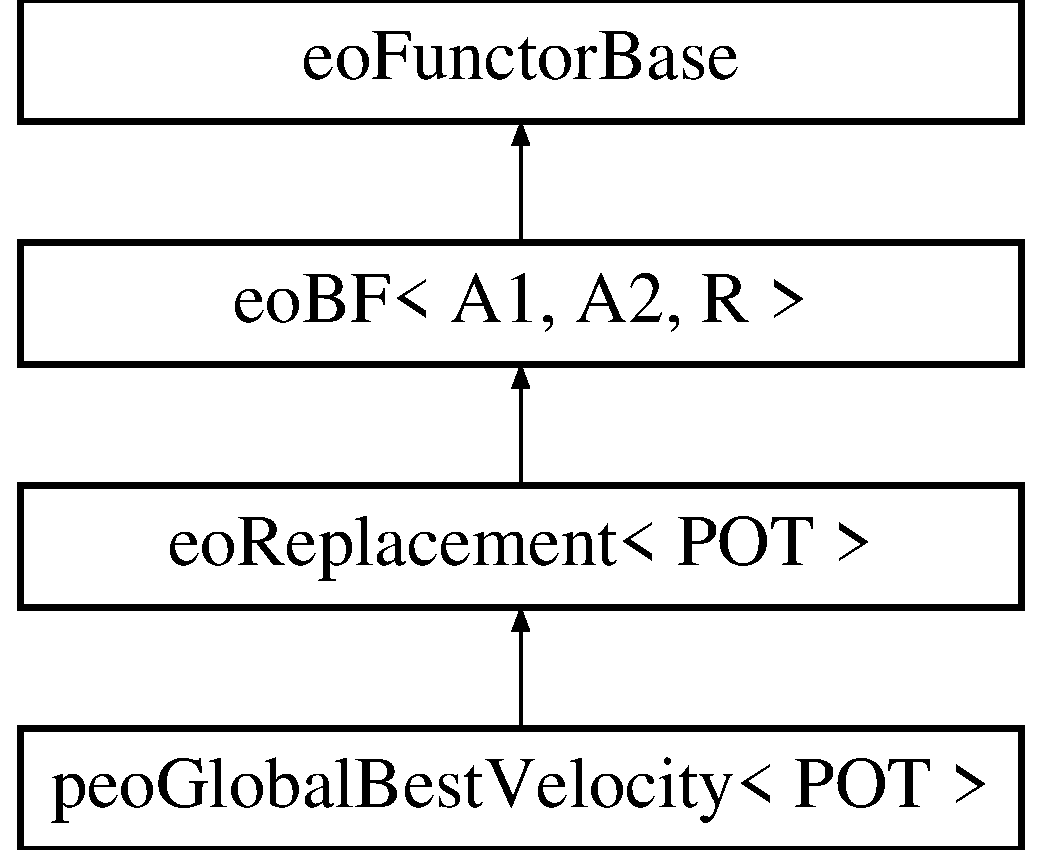
\includegraphics[height=4cm]{classpeoGlobalBestVelocity}
\end{center}
\end{figure}
\subsection*{Public Types}
\begin{CompactItemize}
\item 
\hypertarget{classpeoGlobalBestVelocity_6f80341261df04a504e7926044f1c026}{
typedef POT::Particle\-Velocity\-Type \hyperlink{classpeoGlobalBestVelocity_6f80341261df04a504e7926044f1c026}{Velocity\-Type}}
\label{classpeoGlobalBestVelocity_6f80341261df04a504e7926044f1c026}

\begin{CompactList}\small\item\em typedef : creation of Velocity\-Type \item\end{CompactList}\end{CompactItemize}
\subsection*{Public Member Functions}
\begin{CompactItemize}
\item 
\hyperlink{classpeoGlobalBestVelocity_e43dda9caca16d2aefec72d5d79befe4}{peo\-Global\-Best\-Velocity} (const double \&\_\-c3, \bf{eo\-Velocity}$<$ POT $>$ \&\_\-velocity)
\begin{CompactList}\small\item\em Constructor. \item\end{CompactList}\item 
void \hyperlink{classpeoGlobalBestVelocity_9d8f24594227b59523b4cea4347247b7}{operator()} (\bf{eo\-Pop}$<$ POT $>$ \&\_\-dest, \bf{eo\-Pop}$<$ POT $>$ \&\_\-source)
\begin{CompactList}\small\item\em Virtual operator. \item\end{CompactList}\end{CompactItemize}
\subsection*{Protected Attributes}
\begin{CompactItemize}
\item 
const double \& \hyperlink{classpeoGlobalBestVelocity_d6ff78d4e75ceaa37ede63a55f44d6ce}{c3}
\item 
\hypertarget{classpeoGlobalBestVelocity_c7350b438b27b462b84dad0a2c5edf33}{
\bf{eo\-Velocity}$<$ POT $>$ \& \hyperlink{classpeoGlobalBestVelocity_c7350b438b27b462b84dad0a2c5edf33}{velocity}}
\label{classpeoGlobalBestVelocity_c7350b438b27b462b84dad0a2c5edf33}

\end{CompactItemize}


\subsection{Detailed Description}
\subsubsection*{template$<$class POT$>$ class peo\-Global\-Best\-Velocity$<$ POT $>$}

Specific class for a replacement thanks to the velocity migration of a population of a PSO. 

\begin{Desc}
\item[See also:]\doxyref{eo\-Replacement} \end{Desc}
\begin{Desc}
\item[Version:]1.1 \end{Desc}
\begin{Desc}
\item[Date:]october 2007 \end{Desc}




Definition at line 85 of file peo\-PSO.h.

\subsection{Constructor \& Destructor Documentation}
\hypertarget{classpeoGlobalBestVelocity_e43dda9caca16d2aefec72d5d79befe4}{
\index{peoGlobalBestVelocity@{peo\-Global\-Best\-Velocity}!peoGlobalBestVelocity@{peoGlobalBestVelocity}}
\index{peoGlobalBestVelocity@{peoGlobalBestVelocity}!peoGlobalBestVelocity@{peo\-Global\-Best\-Velocity}}
\subsubsection[peoGlobalBestVelocity]{\setlength{\rightskip}{0pt plus 5cm}template$<$class POT$>$ \hyperlink{classpeoGlobalBestVelocity}{peo\-Global\-Best\-Velocity}$<$ POT $>$::\hyperlink{classpeoGlobalBestVelocity}{peo\-Global\-Best\-Velocity} (const double \& {\em \_\-c3}, \bf{eo\-Velocity}$<$ POT $>$ \& {\em \_\-velocity})\hspace{0.3cm}{\tt  \mbox{[}inline\mbox{]}}}}
\label{classpeoGlobalBestVelocity_e43dda9caca16d2aefec72d5d79befe4}


Constructor. 

\begin{Desc}
\item[Parameters:]
\begin{description}
\item[{\em double}]\& \_\-c3 \item[{\em \doxyref{eo\-Velocity}}]$<$ POT $>$ \&\_\-velocity \end{description}
\end{Desc}


Definition at line 95 of file peo\-PSO.h.

\subsection{Member Function Documentation}
\hypertarget{classpeoGlobalBestVelocity_9d8f24594227b59523b4cea4347247b7}{
\index{peoGlobalBestVelocity@{peo\-Global\-Best\-Velocity}!operator()@{operator()}}
\index{operator()@{operator()}!peoGlobalBestVelocity@{peo\-Global\-Best\-Velocity}}
\subsubsection[operator()]{\setlength{\rightskip}{0pt plus 5cm}template$<$class POT$>$ void \hyperlink{classpeoGlobalBestVelocity}{peo\-Global\-Best\-Velocity}$<$ POT $>$::operator() (\bf{eo\-Pop}$<$ POT $>$ \& {\em \_\-dest}, \bf{eo\-Pop}$<$ POT $>$ \& {\em \_\-source})\hspace{0.3cm}{\tt  \mbox{[}inline\mbox{]}}}}
\label{classpeoGlobalBestVelocity_9d8f24594227b59523b4cea4347247b7}


Virtual operator. 

\begin{Desc}
\item[Parameters:]
\begin{description}
\item[{\em eo\-Pop$<$POT$>$\&}]\_\-dest \item[{\em eo\-Pop$<$POT$>$\&}]\_\-source \end{description}
\end{Desc}


Definition at line 101 of file peo\-PSO.h.

References peo\-Global\-Best\-Velocity$<$ POT $>$::c3, and eo\-Rng::uniform().

\subsection{Member Data Documentation}
\hypertarget{classpeoGlobalBestVelocity_d6ff78d4e75ceaa37ede63a55f44d6ce}{
\index{peoGlobalBestVelocity@{peo\-Global\-Best\-Velocity}!c3@{c3}}
\index{c3@{c3}!peoGlobalBestVelocity@{peo\-Global\-Best\-Velocity}}
\subsubsection[c3]{\setlength{\rightskip}{0pt plus 5cm}template$<$class POT$>$ const double\& \hyperlink{classpeoGlobalBestVelocity}{peo\-Global\-Best\-Velocity}$<$ POT $>$::\hyperlink{classpeoGlobalBestVelocity_d6ff78d4e75ceaa37ede63a55f44d6ce}{c3}\hspace{0.3cm}{\tt  \mbox{[}protected\mbox{]}}}}
\label{classpeoGlobalBestVelocity_d6ff78d4e75ceaa37ede63a55f44d6ce}


\begin{Desc}
\item[Parameters:]
\begin{description}
\item[{\em double}]\& c3 \item[{\em \doxyref{eo\-Velocity}}]$<$ POT $>$ \& velocity \end{description}
\end{Desc}


Definition at line 118 of file peo\-PSO.h.

Referenced by peo\-Global\-Best\-Velocity$<$ POT $>$::operator()().

The documentation for this class was generated from the following file:\begin{CompactItemize}
\item 
peo\-PSO.h\end{CompactItemize}

\include{classpeoMoeoPopEval}
\hypertarget{classpeoMultiStart}{
\section{peo\-Multi\-Start$<$ Entity\-Type $>$ Class Template Reference}
\label{classpeoMultiStart}\index{peoMultiStart@{peoMultiStart}}
}
Class allowing the launch of several algorithms.  


{\tt \#include $<$peo\-Multi\-Start.h$>$}

Inheritance diagram for peo\-Multi\-Start$<$ Entity\-Type $>$::\begin{figure}[H]
\begin{center}
\leavevmode
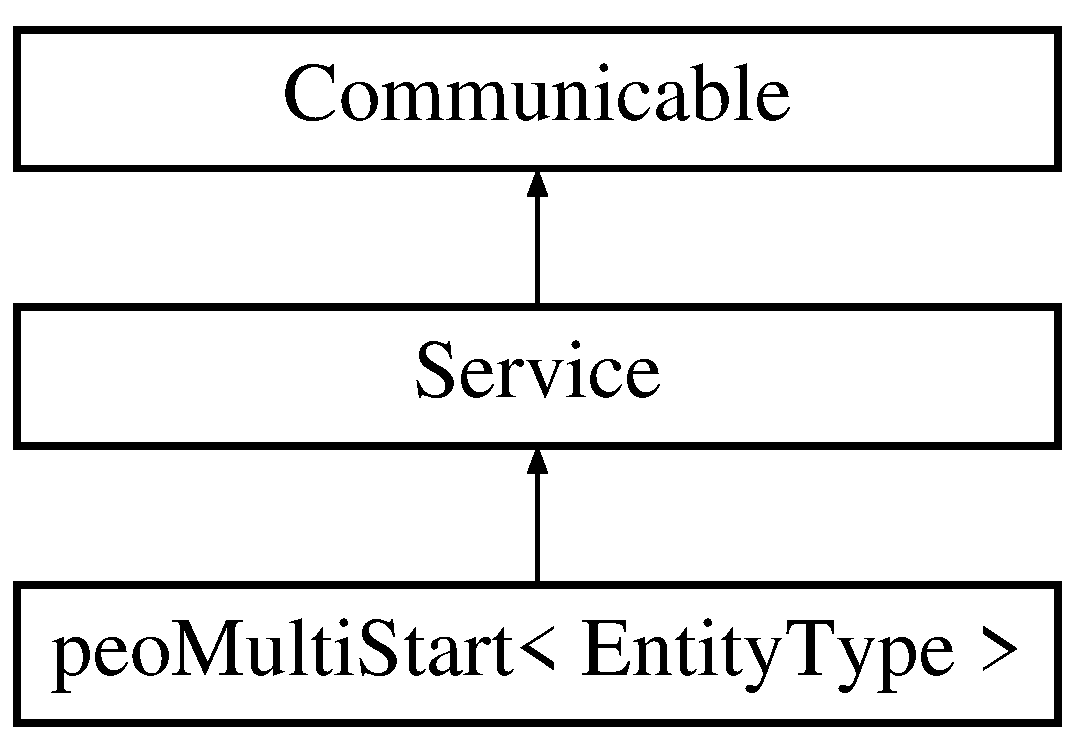
\includegraphics[height=3cm]{classpeoMultiStart}
\end{center}
\end{figure}
\subsection*{Public Member Functions}
\begin{CompactItemize}
\item 
template$<$typename Algorithm\-Type$>$ \hyperlink{classpeoMultiStart_587906a897801d67564b4b4a63798c62}{peo\-Multi\-Start} (Algorithm\-Type \&external\-Algorithm)
\begin{CompactList}\small\item\em Constructor. \item\end{CompactList}\item 
template$<$typename Algorithm\-Return\-Type, typename Algorithm\-Data\-Type$>$ \hyperlink{classpeoMultiStart_0789e7cdcb0cd5f028f4fb531067ceb9}{peo\-Multi\-Start} (Algorithm\-Return\-Type($\ast$external\-Algorithm)(Algorithm\-Data\-Type \&))
\begin{CompactList}\small\item\em Constructor. \item\end{CompactList}\item 
template$<$typename Algorithm\-Type, typename Aggregation\-Function\-Type$>$ \hyperlink{classpeoMultiStart_43de7b0e2bb7a31acf0eb3933a31c612}{peo\-Multi\-Start} (std::vector$<$ Algorithm\-Type $\ast$ $>$ \&external\-Algorithms, Aggregation\-Function\-Type \&external\-Aggregation\-Function)
\begin{CompactList}\small\item\em Constructor. \item\end{CompactList}\item 
template$<$typename Algorithm\-Return\-Type, typename Algorithm\-Data\-Type, typename Aggregation\-Function\-Type$>$ \hyperlink{classpeoMultiStart_81b0be145ca12aec6e75ffd2313bfeab}{peo\-Multi\-Start} (std::vector$<$ Algorithm\-Return\-Type($\ast$)(Algorithm\-Data\-Type \&) $>$ \&external\-Algorithms, Aggregation\-Function\-Type \&external\-Aggregation\-Function)
\begin{CompactList}\small\item\em Constructor. \item\end{CompactList}\item 
\hypertarget{classpeoMultiStart_16a9c5eae2c8ec925738b84bf62b3809}{
\hyperlink{classpeoMultiStart_16a9c5eae2c8ec925738b84bf62b3809}{$\sim$peo\-Multi\-Start} ()}
\label{classpeoMultiStart_16a9c5eae2c8ec925738b84bf62b3809}

\begin{CompactList}\small\item\em Destructor. \item\end{CompactList}\item 
template$<$typename Type$>$ void \hyperlink{classpeoMultiStart_c7410145e7fba059d99da41f5bd5979b}{operator()} (Type \&external\-Data)
\begin{CompactList}\small\item\em operator on the template type \item\end{CompactList}\item 
template$<$typename Type$>$ void \hyperlink{classpeoMultiStart_90ba0e411cafa47b9a306e71319c8365}{operator()} (const Type \&external\-Data\-Begin, const Type \&external\-Data\-End)
\begin{CompactList}\small\item\em operator on the template type \item\end{CompactList}\item 
\hypertarget{classpeoMultiStart_7e2feab3d514259e8c77387b92023f38}{
void \hyperlink{classpeoMultiStart_7e2feab3d514259e8c77387b92023f38}{pack\-Data} ()}
\label{classpeoMultiStart_7e2feab3d514259e8c77387b92023f38}

\begin{CompactList}\small\item\em \doxyref{Function} realizing packages of data. \item\end{CompactList}\item 
\hypertarget{classpeoMultiStart_c8da1b8ae55ee6622fbb9be4f01ee318}{
void \hyperlink{classpeoMultiStart_c8da1b8ae55ee6622fbb9be4f01ee318}{unpack\-Data} ()}
\label{classpeoMultiStart_c8da1b8ae55ee6622fbb9be4f01ee318}

\begin{CompactList}\small\item\em \doxyref{Function} reconstituting packages of data. \item\end{CompactList}\item 
\hypertarget{classpeoMultiStart_ea05cda1b93b07bbb34e121e2fbf7f1d}{
void \hyperlink{classpeoMultiStart_ea05cda1b93b07bbb34e121e2fbf7f1d}{execute} ()}
\label{classpeoMultiStart_ea05cda1b93b07bbb34e121e2fbf7f1d}

\begin{CompactList}\small\item\em \doxyref{Function} which executes the algorithm. \item\end{CompactList}\item 
\hypertarget{classpeoMultiStart_82fcf2bf33e420eb69cb07ec80debd5d}{
void \hyperlink{classpeoMultiStart_82fcf2bf33e420eb69cb07ec80debd5d}{pack\-Result} ()}
\label{classpeoMultiStart_82fcf2bf33e420eb69cb07ec80debd5d}

\begin{CompactList}\small\item\em \doxyref{Function} realizing packages of the result. \item\end{CompactList}\item 
\hypertarget{classpeoMultiStart_4b92ac458ea435e6433e482e8262ba18}{
void \hyperlink{classpeoMultiStart_4b92ac458ea435e6433e482e8262ba18}{unpack\-Result} ()}
\label{classpeoMultiStart_4b92ac458ea435e6433e482e8262ba18}

\begin{CompactList}\small\item\em \doxyref{Function} reconstituting packages of result. \item\end{CompactList}\item 
\hypertarget{classpeoMultiStart_afddf0cc852dbd6dc3a642393ec45207}{
void \hyperlink{classpeoMultiStart_afddf0cc852dbd6dc3a642393ec45207}{notify\-Sending\-Data} ()}
\label{classpeoMultiStart_afddf0cc852dbd6dc3a642393ec45207}

\begin{CompactList}\small\item\em \doxyref{Function} notify\-Sending\-Data. \item\end{CompactList}\item 
\hypertarget{classpeoMultiStart_4baa5a616d1b48ce31834e749aa99431}{
void \hyperlink{classpeoMultiStart_4baa5a616d1b48ce31834e749aa99431}{notify\-Sending\-All\-Resource\-Requests} ()}
\label{classpeoMultiStart_4baa5a616d1b48ce31834e749aa99431}

\begin{CompactList}\small\item\em \doxyref{Function} notify\-Sending\-All\-Resource\-Requests. \item\end{CompactList}\end{CompactItemize}
\subsection*{Private Attributes}
\begin{CompactItemize}
\item 
\hypertarget{classpeoMultiStart_fe3c3b2650dabc5fffac07b4ecbd0081}{
\hyperlink{structpeoMultiStart_1_1AbstractAlgorithm}{Abstract\-Algorithm} $\ast$ \hyperlink{classpeoMultiStart_fe3c3b2650dabc5fffac07b4ecbd0081}{singular\-Algorithm}}
\label{classpeoMultiStart_fe3c3b2650dabc5fffac07b4ecbd0081}

\item 
\hypertarget{classpeoMultiStart_b8c2f3220b82cdba5b19189ebff0a14c}{
std::vector$<$ \hyperlink{structpeoMultiStart_1_1AbstractAlgorithm}{Abstract\-Algorithm} $\ast$ $>$ \hyperlink{classpeoMultiStart_b8c2f3220b82cdba5b19189ebff0a14c}{algorithms}}
\label{classpeoMultiStart_b8c2f3220b82cdba5b19189ebff0a14c}

\item 
\hypertarget{classpeoMultiStart_eb60fb5f72a95b8fffc5c7012e8b2ce8}{
\hyperlink{structpeoMultiStart_1_1AbstractAggregationAlgorithm}{Abstract\-Aggregation\-Algorithm} $\ast$ \hyperlink{classpeoMultiStart_eb60fb5f72a95b8fffc5c7012e8b2ce8}{aggregation\-Function}}
\label{classpeoMultiStart_eb60fb5f72a95b8fffc5c7012e8b2ce8}

\item 
\hypertarget{classpeoMultiStart_8f43aa54645797e718510bb172c3cf5e}{
Entity\-Type \hyperlink{classpeoMultiStart_8f43aa54645797e718510bb172c3cf5e}{entity\-Type\-Instance}}
\label{classpeoMultiStart_8f43aa54645797e718510bb172c3cf5e}

\item 
\hypertarget{classpeoMultiStart_2f40db0afb4a657f2d6cf10b83dcb2c3}{
std::vector$<$ \hyperlink{structpeoMultiStart_1_1AbstractDataType}{Abstract\-Data\-Type} $\ast$ $>$ \hyperlink{classpeoMultiStart_2f40db0afb4a657f2d6cf10b83dcb2c3}{data}}
\label{classpeoMultiStart_2f40db0afb4a657f2d6cf10b83dcb2c3}

\item 
\hypertarget{classpeoMultiStart_ee265c52dd3597b8b6a2ab9d5c38afce}{
unsigned \hyperlink{classpeoMultiStart_ee265c52dd3597b8b6a2ab9d5c38afce}{idx}}
\label{classpeoMultiStart_ee265c52dd3597b8b6a2ab9d5c38afce}

\item 
\hypertarget{classpeoMultiStart_6054f4cdb5fd12edd4c4fb0e358eb4f7}{
unsigned \hyperlink{classpeoMultiStart_6054f4cdb5fd12edd4c4fb0e358eb4f7}{num\_\-term}}
\label{classpeoMultiStart_6054f4cdb5fd12edd4c4fb0e358eb4f7}

\item 
\hypertarget{classpeoMultiStart_a4b6398ee90389ca5ed997f56b77d69f}{
unsigned \hyperlink{classpeoMultiStart_a4b6398ee90389ca5ed997f56b77d69f}{data\-Index}}
\label{classpeoMultiStart_a4b6398ee90389ca5ed997f56b77d69f}

\item 
\hypertarget{classpeoMultiStart_872b786b612470d0d07490830465f70e}{
unsigned \hyperlink{classpeoMultiStart_872b786b612470d0d07490830465f70e}{function\-Index}}
\label{classpeoMultiStart_872b786b612470d0d07490830465f70e}

\end{CompactItemize}
\subsection*{Classes}
\begin{CompactItemize}
\item 
struct \hyperlink{structpeoMultiStart_1_1AbstractAggregationAlgorithm}{Abstract\-Aggregation\-Algorithm}
\item 
struct \hyperlink{structpeoMultiStart_1_1AbstractAlgorithm}{Abstract\-Algorithm}
\item 
struct \hyperlink{structpeoMultiStart_1_1AbstractDataType}{Abstract\-Data\-Type}
\item 
struct \hyperlink{structpeoMultiStart_1_1AggregationAlgorithm}{Aggregation\-Algorithm}
\item 
struct \hyperlink{structpeoMultiStart_1_1Algorithm}{Algorithm}
\item 
struct \hyperlink{structpeoMultiStart_1_1DataType}{Data\-Type}
\item 
struct \hyperlink{structpeoMultiStart_1_1FunctionAlgorithm}{Function\-Algorithm}
\item 
struct \hyperlink{structpeoMultiStart_1_1NoAggregationFunction}{No\-Aggregation\-Function}
\end{CompactItemize}


\subsection{Detailed Description}
\subsubsection*{template$<$typename Entity\-Type$>$ class peo\-Multi\-Start$<$ Entity\-Type $>$}

Class allowing the launch of several algorithms. 

\begin{Desc}
\item[See also:]\hyperlink{classService}{Service} \end{Desc}
\begin{Desc}
\item[Version:]1.1 \end{Desc}
\begin{Desc}
\item[Date:]january 2008 \end{Desc}




Definition at line 49 of file peo\-Multi\-Start.h.

\subsection{Constructor \& Destructor Documentation}
\hypertarget{classpeoMultiStart_587906a897801d67564b4b4a63798c62}{
\index{peoMultiStart@{peo\-Multi\-Start}!peoMultiStart@{peoMultiStart}}
\index{peoMultiStart@{peoMultiStart}!peoMultiStart@{peo\-Multi\-Start}}
\subsubsection[peoMultiStart]{\setlength{\rightskip}{0pt plus 5cm}template$<$typename Entity\-Type$>$ template$<$typename Algorithm\-Type$>$ \hyperlink{classpeoMultiStart}{peo\-Multi\-Start}$<$ Entity\-Type $>$::\hyperlink{classpeoMultiStart}{peo\-Multi\-Start} (Algorithm\-Type \& {\em external\-Algorithm})\hspace{0.3cm}{\tt  \mbox{[}inline\mbox{]}}}}
\label{classpeoMultiStart_587906a897801d67564b4b4a63798c62}


Constructor. 

\begin{Desc}
\item[Parameters:]
\begin{description}
\item[{\em Algorithm\-Type\&}]external\-Algorithm \end{description}
\end{Desc}


Definition at line 56 of file peo\-Multi\-Start.h.

References peo\-Multi\-Start$<$ Entity\-Type $>$::aggregation\-Function, peo\-Multi\-Start$<$ Entity\-Type $>$::algorithms, and peo\-Multi\-Start$<$ Entity\-Type $>$::singular\-Algorithm.\hypertarget{classpeoMultiStart_0789e7cdcb0cd5f028f4fb531067ceb9}{
\index{peoMultiStart@{peo\-Multi\-Start}!peoMultiStart@{peoMultiStart}}
\index{peoMultiStart@{peoMultiStart}!peoMultiStart@{peo\-Multi\-Start}}
\subsubsection[peoMultiStart]{\setlength{\rightskip}{0pt plus 5cm}template$<$typename Entity\-Type$>$ template$<$typename Algorithm\-Return\-Type, typename Algorithm\-Data\-Type$>$ \hyperlink{classpeoMultiStart}{peo\-Multi\-Start}$<$ Entity\-Type $>$::\hyperlink{classpeoMultiStart}{peo\-Multi\-Start} (Algorithm\-Return\-Type($\ast$)(Algorithm\-Data\-Type \&) {\em external\-Algorithm})\hspace{0.3cm}{\tt  \mbox{[}inline\mbox{]}}}}
\label{classpeoMultiStart_0789e7cdcb0cd5f028f4fb531067ceb9}


Constructor. 

\begin{Desc}
\item[Parameters:]
\begin{description}
\item[{\em Algorithm\-Return\-Type}]($\ast$external\-Algorithm)( Algorithm\-Data\-Type\& ) \end{description}
\end{Desc}


Definition at line 65 of file peo\-Multi\-Start.h.

References peo\-Multi\-Start$<$ Entity\-Type $>$::aggregation\-Function, peo\-Multi\-Start$<$ Entity\-Type $>$::algorithms, and peo\-Multi\-Start$<$ Entity\-Type $>$::singular\-Algorithm.\hypertarget{classpeoMultiStart_43de7b0e2bb7a31acf0eb3933a31c612}{
\index{peoMultiStart@{peo\-Multi\-Start}!peoMultiStart@{peoMultiStart}}
\index{peoMultiStart@{peoMultiStart}!peoMultiStart@{peo\-Multi\-Start}}
\subsubsection[peoMultiStart]{\setlength{\rightskip}{0pt plus 5cm}template$<$typename Entity\-Type$>$ template$<$typename Algorithm\-Type, typename Aggregation\-Function\-Type$>$ \hyperlink{classpeoMultiStart}{peo\-Multi\-Start}$<$ Entity\-Type $>$::\hyperlink{classpeoMultiStart}{peo\-Multi\-Start} (std::vector$<$ Algorithm\-Type $\ast$ $>$ \& {\em external\-Algorithms}, Aggregation\-Function\-Type \& {\em external\-Aggregation\-Function})\hspace{0.3cm}{\tt  \mbox{[}inline\mbox{]}}}}
\label{classpeoMultiStart_43de7b0e2bb7a31acf0eb3933a31c612}


Constructor. 

\begin{Desc}
\item[Parameters:]
\begin{description}
\item[{\em std::vector$<$}]Algorithm\-Type$\ast$ $>$\& external\-Algorithms \item[{\em Aggregation\-Function\-Type\&}]external\-Aggregation\-Function \end{description}
\end{Desc}


Definition at line 75 of file peo\-Multi\-Start.h.

References peo\-Multi\-Start$<$ Entity\-Type $>$::aggregation\-Function, and peo\-Multi\-Start$<$ Entity\-Type $>$::algorithms.\hypertarget{classpeoMultiStart_81b0be145ca12aec6e75ffd2313bfeab}{
\index{peoMultiStart@{peo\-Multi\-Start}!peoMultiStart@{peoMultiStart}}
\index{peoMultiStart@{peoMultiStart}!peoMultiStart@{peo\-Multi\-Start}}
\subsubsection[peoMultiStart]{\setlength{\rightskip}{0pt plus 5cm}template$<$typename Entity\-Type$>$ template$<$typename Algorithm\-Return\-Type, typename Algorithm\-Data\-Type, typename Aggregation\-Function\-Type$>$ \hyperlink{classpeoMultiStart}{peo\-Multi\-Start}$<$ Entity\-Type $>$::\hyperlink{classpeoMultiStart}{peo\-Multi\-Start} (std::vector$<$ Algorithm\-Return\-Type($\ast$)(Algorithm\-Data\-Type \&) $>$ \& {\em external\-Algorithms}, Aggregation\-Function\-Type \& {\em external\-Aggregation\-Function})\hspace{0.3cm}{\tt  \mbox{[}inline\mbox{]}}}}
\label{classpeoMultiStart_81b0be145ca12aec6e75ffd2313bfeab}


Constructor. 

\begin{Desc}
\item[Parameters:]
\begin{description}
\item[{\em std::vector$<$}]Algorithm\-Return\-Type ($\ast$)( Algorithm\-Data\-Type\& ) $>$\& external\-Algorithms \item[{\em Aggregation\-Function\-Type\&}]external\-Aggregation\-Function \end{description}
\end{Desc}


Definition at line 87 of file peo\-Multi\-Start.h.

References peo\-Multi\-Start$<$ Entity\-Type $>$::aggregation\-Function, and peo\-Multi\-Start$<$ Entity\-Type $>$::algorithms.

\subsection{Member Function Documentation}
\hypertarget{classpeoMultiStart_c7410145e7fba059d99da41f5bd5979b}{
\index{peoMultiStart@{peo\-Multi\-Start}!operator()@{operator()}}
\index{operator()@{operator()}!peoMultiStart@{peo\-Multi\-Start}}
\subsubsection[operator()]{\setlength{\rightskip}{0pt plus 5cm}template$<$typename Entity\-Type$>$ template$<$typename Type$>$ void \hyperlink{classpeoMultiStart}{peo\-Multi\-Start}$<$ Entity\-Type $>$::operator() (Type \& {\em external\-Data})\hspace{0.3cm}{\tt  \mbox{[}inline\mbox{]}}}}
\label{classpeoMultiStart_c7410145e7fba059d99da41f5bd5979b}


operator on the template type 

\begin{Desc}
\item[Parameters:]
\begin{description}
\item[{\em Type\&}]external\-Data \end{description}
\end{Desc}


Definition at line 106 of file peo\-Multi\-Start.h.

References peo\-Multi\-Start$<$ Entity\-Type $>$::algorithms, peo\-Multi\-Start$<$ Entity\-Type $>$::data, peo\-Multi\-Start$<$ Entity\-Type $>$::data\-Index, peo\-Multi\-Start$<$ Entity\-Type $>$::function\-Index, peo\-Multi\-Start$<$ Entity\-Type $>$::idx, peo\-Multi\-Start$<$ Entity\-Type $>$::num\_\-term, Service::request\-Resource\-Request(), and Communicable::stop().\hypertarget{classpeoMultiStart_90ba0e411cafa47b9a306e71319c8365}{
\index{peoMultiStart@{peo\-Multi\-Start}!operator()@{operator()}}
\index{operator()@{operator()}!peoMultiStart@{peo\-Multi\-Start}}
\subsubsection[operator()]{\setlength{\rightskip}{0pt plus 5cm}template$<$typename Entity\-Type$>$ template$<$typename Type$>$ void \hyperlink{classpeoMultiStart}{peo\-Multi\-Start}$<$ Entity\-Type $>$::operator() (const Type \& {\em external\-Data\-Begin}, const Type \& {\em external\-Data\-End})\hspace{0.3cm}{\tt  \mbox{[}inline\mbox{]}}}}
\label{classpeoMultiStart_90ba0e411cafa47b9a306e71319c8365}


operator on the template type 

\begin{Desc}
\item[Parameters:]
\begin{description}
\item[{\em Type\&}]external\-Data\-Begin \item[{\em Type\&}]external\-Data\-End \end{description}
\end{Desc}


Definition at line 120 of file peo\-Multi\-Start.h.

References peo\-Multi\-Start$<$ Entity\-Type $>$::algorithms, peo\-Multi\-Start$<$ Entity\-Type $>$::data, peo\-Multi\-Start$<$ Entity\-Type $>$::data\-Index, peo\-Multi\-Start$<$ Entity\-Type $>$::function\-Index, peo\-Multi\-Start$<$ Entity\-Type $>$::idx, peo\-Multi\-Start$<$ Entity\-Type $>$::num\_\-term, Service::request\-Resource\-Request(), and Communicable::stop().

The documentation for this class was generated from the following file:\begin{CompactItemize}
\item 
peo\-Multi\-Start.h\end{CompactItemize}

\hypertarget{structpeoMultiStart_1_1AbstractAggregationAlgorithm}{
\section{peo\-Multi\-Start$<$ Entity\-Type $>$::Abstract\-Aggregation\-Algorithm Struct Reference}
\label{structpeoMultiStart_1_1AbstractAggregationAlgorithm}\index{peoMultiStart::AbstractAggregationAlgorithm@{peoMultiStart::AbstractAggregationAlgorithm}}
}
Inheritance diagram for peo\-Multi\-Start$<$ Entity\-Type $>$::Abstract\-Aggregation\-Algorithm::\begin{figure}[H]
\begin{center}
\leavevmode
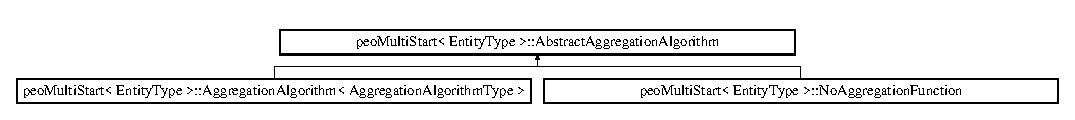
\includegraphics[height=1.1691cm]{structpeoMultiStart_1_1AbstractAggregationAlgorithm}
\end{center}
\end{figure}
\subsection*{Public Member Functions}
\begin{CompactItemize}
\item 
\hypertarget{structpeoMultiStart_1_1AbstractAggregationAlgorithm_58cbddc4a83735f15ff617a0a3121439}{
virtual \hyperlink{structpeoMultiStart_1_1AbstractAggregationAlgorithm_58cbddc4a83735f15ff617a0a3121439}{$\sim$Abstract\-Aggregation\-Algorithm} ()}
\label{structpeoMultiStart_1_1AbstractAggregationAlgorithm_58cbddc4a83735f15ff617a0a3121439}

\item 
\hypertarget{structpeoMultiStart_1_1AbstractAggregationAlgorithm_3122e126ba11de97e98563400482ae68}{
virtual void \hyperlink{structpeoMultiStart_1_1AbstractAggregationAlgorithm_3122e126ba11de97e98563400482ae68}{operator()} (\hyperlink{structpeoMultiStart_1_1AbstractDataType}{Abstract\-Data\-Type} \&data\-Type\-Instance\-A, \hyperlink{structpeoMultiStart_1_1AbstractDataType}{Abstract\-Data\-Type} \&data\-Type\-Instance\-B)}
\label{structpeoMultiStart_1_1AbstractAggregationAlgorithm_3122e126ba11de97e98563400482ae68}

\end{CompactItemize}


\subsection{Detailed Description}
\subsubsection*{template$<$typename Entity\-Type$>$ struct peo\-Multi\-Start$<$ Entity\-Type $>$::Abstract\-Aggregation\-Algorithm}





Definition at line 205 of file peo\-Multi\-Start.h.

The documentation for this struct was generated from the following file:\begin{CompactItemize}
\item 
peo\-Multi\-Start.h\end{CompactItemize}

\hypertarget{structpeoMultiStart_1_1AbstractAlgorithm}{
\section{peo\-Multi\-Start$<$ Entity\-Type $>$::Abstract\-Algorithm Struct Reference}
\label{structpeoMultiStart_1_1AbstractAlgorithm}\index{peoMultiStart::AbstractAlgorithm@{peoMultiStart::AbstractAlgorithm}}
}
Inheritance diagram for peo\-Multi\-Start$<$ Entity\-Type $>$::Abstract\-Algorithm::\begin{figure}[H]
\begin{center}
\leavevmode
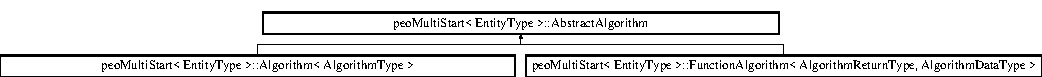
\includegraphics[height=1.03131cm]{structpeoMultiStart_1_1AbstractAlgorithm}
\end{center}
\end{figure}
\subsection*{Public Member Functions}
\begin{CompactItemize}
\item 
\hypertarget{structpeoMultiStart_1_1AbstractAlgorithm_0371e92bf1c07a89d9fd1534cc74e63e}{
virtual \hyperlink{structpeoMultiStart_1_1AbstractAlgorithm_0371e92bf1c07a89d9fd1534cc74e63e}{$\sim$Abstract\-Algorithm} ()}
\label{structpeoMultiStart_1_1AbstractAlgorithm_0371e92bf1c07a89d9fd1534cc74e63e}

\item 
\hypertarget{structpeoMultiStart_1_1AbstractAlgorithm_3832720a3e6869784fc906c7bda2313c}{
virtual void \hyperlink{structpeoMultiStart_1_1AbstractAlgorithm_3832720a3e6869784fc906c7bda2313c}{operator()} (\hyperlink{structpeoMultiStart_1_1AbstractDataType}{Abstract\-Data\-Type} \&data\-Type\-Instance)}
\label{structpeoMultiStart_1_1AbstractAlgorithm_3832720a3e6869784fc906c7bda2313c}

\end{CompactItemize}


\subsection{Detailed Description}
\subsubsection*{template$<$typename Entity\-Type$>$ struct peo\-Multi\-Start$<$ Entity\-Type $>$::Abstract\-Algorithm}





Definition at line 175 of file peo\-Multi\-Start.h.

The documentation for this struct was generated from the following file:\begin{CompactItemize}
\item 
peo\-Multi\-Start.h\end{CompactItemize}

\hypertarget{structpeoMultiStart_1_1AbstractDataType}{
\section{peo\-Multi\-Start$<$ Entity\-Type $>$::Abstract\-Data\-Type Struct Reference}
\label{structpeoMultiStart_1_1AbstractDataType}\index{peoMultiStart::AbstractDataType@{peoMultiStart::AbstractDataType}}
}
Inheritance diagram for peo\-Multi\-Start$<$ Entity\-Type $>$::Abstract\-Data\-Type::\begin{figure}[H]
\begin{center}
\leavevmode
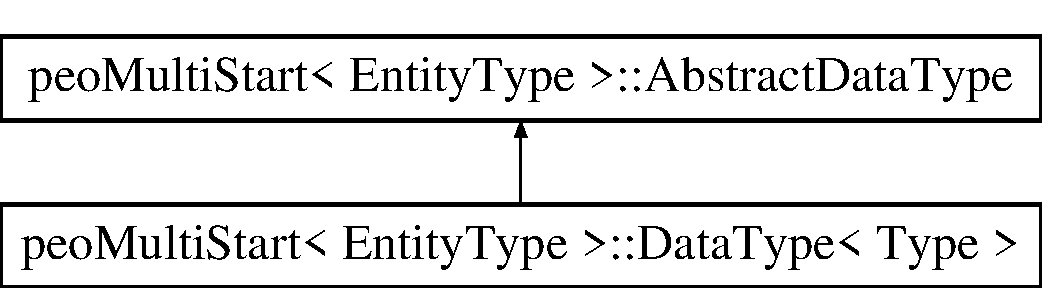
\includegraphics[height=2cm]{structpeoMultiStart_1_1AbstractDataType}
\end{center}
\end{figure}
\subsection*{Public Member Functions}
\begin{CompactItemize}
\item 
\hypertarget{structpeoMultiStart_1_1AbstractDataType_d1ff4bf7da5330c7f4395f9e3c9c29bd}{
virtual \hyperlink{structpeoMultiStart_1_1AbstractDataType_d1ff4bf7da5330c7f4395f9e3c9c29bd}{$\sim$Abstract\-Data\-Type} ()}
\label{structpeoMultiStart_1_1AbstractDataType_d1ff4bf7da5330c7f4395f9e3c9c29bd}

\item 
\hypertarget{structpeoMultiStart_1_1AbstractDataType_e5fe4d7fa98c492bc748176780790d93}{
template$<$typename Type$>$ \hyperlink{structpeoMultiStart_1_1AbstractDataType_e5fe4d7fa98c492bc748176780790d93}{operator Type \&} ()}
\label{structpeoMultiStart_1_1AbstractDataType_e5fe4d7fa98c492bc748176780790d93}

\end{CompactItemize}


\subsection{Detailed Description}
\subsubsection*{template$<$typename Entity\-Type$>$ struct peo\-Multi\-Start$<$ Entity\-Type $>$::Abstract\-Data\-Type}





Definition at line 158 of file peo\-Multi\-Start.h.

The documentation for this struct was generated from the following file:\begin{CompactItemize}
\item 
peo\-Multi\-Start.h\end{CompactItemize}

\hypertarget{structpeoMultiStart_1_1AggregationAlgorithm}{
\section{peo\-Multi\-Start$<$ Entity\-Type $>$::Aggregation\-Algorithm$<$ Aggregation\-Algorithm\-Type $>$ Struct Template Reference}
\label{structpeoMultiStart_1_1AggregationAlgorithm}\index{peoMultiStart::AggregationAlgorithm@{peoMultiStart::AggregationAlgorithm}}
}
Inheritance diagram for peo\-Multi\-Start$<$ Entity\-Type $>$::Aggregation\-Algorithm$<$ Aggregation\-Algorithm\-Type $>$::\begin{figure}[H]
\begin{center}
\leavevmode
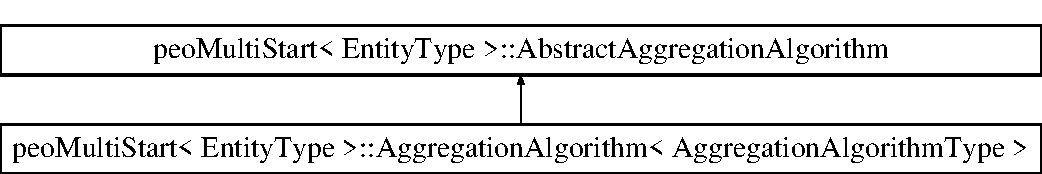
\includegraphics[height=2cm]{structpeoMultiStart_1_1AggregationAlgorithm}
\end{center}
\end{figure}
\subsection*{Public Member Functions}
\begin{CompactItemize}
\item 
\hypertarget{structpeoMultiStart_1_1AggregationAlgorithm_2465c461bfcd70c60db220b848ef76da}{
\hyperlink{structpeoMultiStart_1_1AggregationAlgorithm_2465c461bfcd70c60db220b848ef76da}{Aggregation\-Algorithm} (Aggregation\-Algorithm\-Type \&external\-Aggregation\-Algorithm)}
\label{structpeoMultiStart_1_1AggregationAlgorithm_2465c461bfcd70c60db220b848ef76da}

\item 
\hypertarget{structpeoMultiStart_1_1AggregationAlgorithm_5c095e1e53c6803e7e1fd8b749ec9758}{
void \hyperlink{structpeoMultiStart_1_1AggregationAlgorithm_5c095e1e53c6803e7e1fd8b749ec9758}{operator()} (\hyperlink{structpeoMultiStart_1_1AbstractDataType}{Abstract\-Data\-Type} \&data\-Type\-Instance\-A, \hyperlink{structpeoMultiStart_1_1AbstractDataType}{Abstract\-Data\-Type} \&data\-Type\-Instance\-B)}
\label{structpeoMultiStart_1_1AggregationAlgorithm_5c095e1e53c6803e7e1fd8b749ec9758}

\end{CompactItemize}
\subsection*{Public Attributes}
\begin{CompactItemize}
\item 
\hypertarget{structpeoMultiStart_1_1AggregationAlgorithm_84bd7251c4f117fdbb3bbd68d90f6d35}{
Aggregation\-Algorithm\-Type \& \hyperlink{structpeoMultiStart_1_1AggregationAlgorithm_84bd7251c4f117fdbb3bbd68d90f6d35}{aggregation\-Algorithm}}
\label{structpeoMultiStart_1_1AggregationAlgorithm_84bd7251c4f117fdbb3bbd68d90f6d35}

\end{CompactItemize}


\subsection{Detailed Description}
\subsubsection*{template$<$typename Entity\-Type$>$template$<$typename Aggregation\-Algorithm\-Type$>$ struct peo\-Multi\-Start$<$ Entity\-Type $>$::Aggregation\-Algorithm$<$ Aggregation\-Algorithm\-Type $>$}





Definition at line 213 of file peo\-Multi\-Start.h.

The documentation for this struct was generated from the following file:\begin{CompactItemize}
\item 
peo\-Multi\-Start.h\end{CompactItemize}

\hypertarget{structpeoMultiStart_1_1Algorithm}{
\section{peo\-Multi\-Start$<$ Entity\-Type $>$::Algorithm$<$ Algorithm\-Type $>$ Struct Template Reference}
\label{structpeoMultiStart_1_1Algorithm}\index{peoMultiStart::Algorithm@{peoMultiStart::Algorithm}}
}
Inheritance diagram for peo\-Multi\-Start$<$ Entity\-Type $>$::Algorithm$<$ Algorithm\-Type $>$::\begin{figure}[H]
\begin{center}
\leavevmode
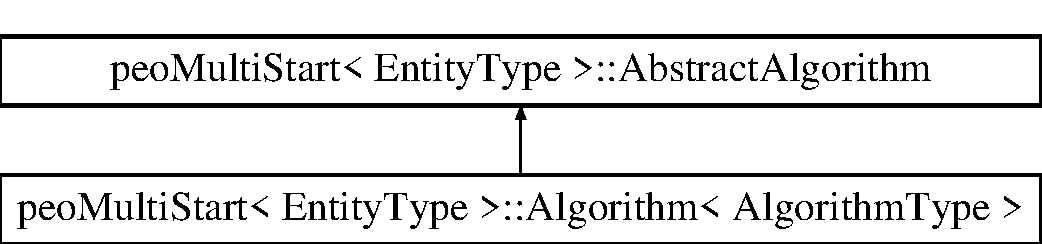
\includegraphics[height=2cm]{structpeoMultiStart_1_1Algorithm}
\end{center}
\end{figure}
\subsection*{Public Member Functions}
\begin{CompactItemize}
\item 
\hypertarget{structpeoMultiStart_1_1Algorithm_39f0818e387b39c70432a96f512482ec}{
\hyperlink{structpeoMultiStart_1_1Algorithm_39f0818e387b39c70432a96f512482ec}{Algorithm} (Algorithm\-Type \&external\-Algorithm)}
\label{structpeoMultiStart_1_1Algorithm_39f0818e387b39c70432a96f512482ec}

\item 
\hypertarget{structpeoMultiStart_1_1Algorithm_73dc7bef0b4e1430910383ba51a3c4d4}{
void \hyperlink{structpeoMultiStart_1_1Algorithm_73dc7bef0b4e1430910383ba51a3c4d4}{operator()} (\hyperlink{structpeoMultiStart_1_1AbstractDataType}{Abstract\-Data\-Type} \&data\-Type\-Instance)}
\label{structpeoMultiStart_1_1Algorithm_73dc7bef0b4e1430910383ba51a3c4d4}

\end{CompactItemize}
\subsection*{Public Attributes}
\begin{CompactItemize}
\item 
\hypertarget{structpeoMultiStart_1_1Algorithm_e7a6e014c00ef0a7df5d429aba4f5f96}{
Algorithm\-Type \& \hyperlink{structpeoMultiStart_1_1Algorithm_e7a6e014c00ef0a7df5d429aba4f5f96}{algorithm}}
\label{structpeoMultiStart_1_1Algorithm_e7a6e014c00ef0a7df5d429aba4f5f96}

\end{CompactItemize}


\subsection{Detailed Description}
\subsubsection*{template$<$typename Entity\-Type$>$template$<$typename Algorithm\-Type$>$ struct peo\-Multi\-Start$<$ Entity\-Type $>$::Algorithm$<$ Algorithm\-Type $>$}





Definition at line 183 of file peo\-Multi\-Start.h.

The documentation for this struct was generated from the following file:\begin{CompactItemize}
\item 
peo\-Multi\-Start.h\end{CompactItemize}

\hypertarget{structpeoMultiStart_1_1DataType}{
\section{peo\-Multi\-Start$<$ Entity\-Type $>$::Data\-Type$<$ Type $>$ Struct Template Reference}
\label{structpeoMultiStart_1_1DataType}\index{peoMultiStart::DataType@{peoMultiStart::DataType}}
}
Inheritance diagram for peo\-Multi\-Start$<$ Entity\-Type $>$::Data\-Type$<$ Type $>$::\begin{figure}[H]
\begin{center}
\leavevmode
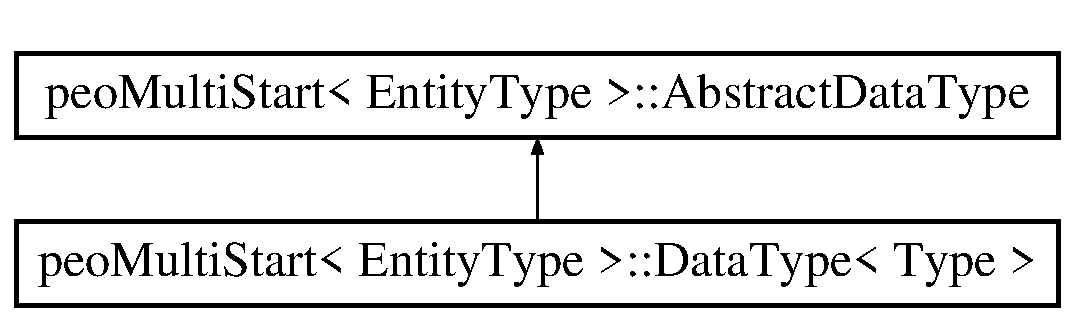
\includegraphics[height=2cm]{structpeoMultiStart_1_1DataType}
\end{center}
\end{figure}
\subsection*{Public Member Functions}
\begin{CompactItemize}
\item 
\hypertarget{structpeoMultiStart_1_1DataType_58e7f3b359440b8b1e10d8ca04dbb294}{
\hyperlink{structpeoMultiStart_1_1DataType_58e7f3b359440b8b1e10d8ca04dbb294}{Data\-Type} (Type \&external\-Data)}
\label{structpeoMultiStart_1_1DataType_58e7f3b359440b8b1e10d8ca04dbb294}

\end{CompactItemize}
\subsection*{Public Attributes}
\begin{CompactItemize}
\item 
\hypertarget{structpeoMultiStart_1_1DataType_a071f9676f4ed8bdd3bc58c1e66ec378}{
Type \& \hyperlink{structpeoMultiStart_1_1DataType_a071f9676f4ed8bdd3bc58c1e66ec378}{data}}
\label{structpeoMultiStart_1_1DataType_a071f9676f4ed8bdd3bc58c1e66ec378}

\end{CompactItemize}


\subsection{Detailed Description}
\subsubsection*{template$<$typename Entity\-Type$>$template$<$typename Type$>$ struct peo\-Multi\-Start$<$ Entity\-Type $>$::Data\-Type$<$ Type $>$}





Definition at line 168 of file peo\-Multi\-Start.h.

The documentation for this struct was generated from the following file:\begin{CompactItemize}
\item 
peo\-Multi\-Start.h\end{CompactItemize}

\hypertarget{structpeoMultiStart_1_1FunctionAlgorithm}{
\section{peo\-Multi\-Start$<$ Entity\-Type $>$::Function\-Algorithm$<$ Algorithm\-Return\-Type, Algorithm\-Data\-Type $>$ Struct Template Reference}
\label{structpeoMultiStart_1_1FunctionAlgorithm}\index{peoMultiStart::FunctionAlgorithm@{peoMultiStart::FunctionAlgorithm}}
}
Inheritance diagram for peo\-Multi\-Start$<$ Entity\-Type $>$::Function\-Algorithm$<$ Algorithm\-Return\-Type, Algorithm\-Data\-Type $>$::\begin{figure}[H]
\begin{center}
\leavevmode
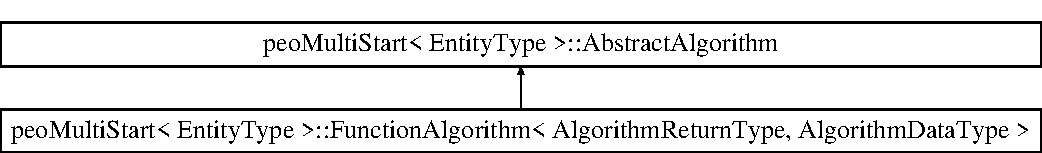
\includegraphics[height=2cm]{structpeoMultiStart_1_1FunctionAlgorithm}
\end{center}
\end{figure}
\subsection*{Public Member Functions}
\begin{CompactItemize}
\item 
\hypertarget{structpeoMultiStart_1_1FunctionAlgorithm_e17b79bb29dd4f6f2f827970c5aba5fd}{
\hyperlink{structpeoMultiStart_1_1FunctionAlgorithm_e17b79bb29dd4f6f2f827970c5aba5fd}{Function\-Algorithm} (Algorithm\-Return\-Type($\ast$external\-Algorithm)(Algorithm\-Data\-Type \&))}
\label{structpeoMultiStart_1_1FunctionAlgorithm_e17b79bb29dd4f6f2f827970c5aba5fd}

\item 
\hypertarget{structpeoMultiStart_1_1FunctionAlgorithm_134a61668ce76ed36c5d1d454c6b3b43}{
void \hyperlink{structpeoMultiStart_1_1FunctionAlgorithm_134a61668ce76ed36c5d1d454c6b3b43}{operator()} (\hyperlink{structpeoMultiStart_1_1AbstractDataType}{Abstract\-Data\-Type} \&data\-Type\-Instance)}
\label{structpeoMultiStart_1_1FunctionAlgorithm_134a61668ce76ed36c5d1d454c6b3b43}

\end{CompactItemize}


\subsection{Detailed Description}
\subsubsection*{template$<$typename Entity\-Type$>$template$<$typename Algorithm\-Return\-Type, typename Algorithm\-Data\-Type$>$ struct peo\-Multi\-Start$<$ Entity\-Type $>$::Function\-Algorithm$<$ Algorithm\-Return\-Type, Algorithm\-Data\-Type $>$}





Definition at line 194 of file peo\-Multi\-Start.h.

The documentation for this struct was generated from the following file:\begin{CompactItemize}
\item 
peo\-Multi\-Start.h\end{CompactItemize}

\hypertarget{structpeoMultiStart_1_1NoAggregationFunction}{
\section{peo\-Multi\-Start$<$ Entity\-Type $>$::No\-Aggregation\-Function Struct Reference}
\label{structpeoMultiStart_1_1NoAggregationFunction}\index{peoMultiStart::NoAggregationFunction@{peoMultiStart::NoAggregationFunction}}
}
Inheritance diagram for peo\-Multi\-Start$<$ Entity\-Type $>$::No\-Aggregation\-Function::\begin{figure}[H]
\begin{center}
\leavevmode
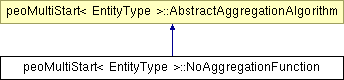
\includegraphics[height=2cm]{structpeoMultiStart_1_1NoAggregationFunction}
\end{center}
\end{figure}
\subsection*{Public Member Functions}
\begin{CompactItemize}
\item 
\hypertarget{structpeoMultiStart_1_1NoAggregationFunction_985f527d01dcc73e2c600b7293ace1c7}{
void \hyperlink{structpeoMultiStart_1_1NoAggregationFunction_985f527d01dcc73e2c600b7293ace1c7}{operator()} (\hyperlink{structpeoMultiStart_1_1AbstractDataType}{Abstract\-Data\-Type} \&data\-Type\-Instance\-A, \hyperlink{structpeoMultiStart_1_1AbstractDataType}{Abstract\-Data\-Type} \&data\-Type\-Instance\-B)}
\label{structpeoMultiStart_1_1NoAggregationFunction_985f527d01dcc73e2c600b7293ace1c7}

\end{CompactItemize}


\subsection{Detailed Description}
\subsubsection*{template$<$typename Entity\-Type$>$ struct peo\-Multi\-Start$<$ Entity\-Type $>$::No\-Aggregation\-Function}





Definition at line 224 of file peo\-Multi\-Start.h.

The documentation for this struct was generated from the following file:\begin{CompactItemize}
\item 
peo\-Multi\-Start.h\end{CompactItemize}

\hypertarget{classpeoNoAggEvalFunc}{
\section{peo\-No\-Agg\-Eval\-Func$<$ EOT $>$ Class Template Reference}
\label{classpeoNoAggEvalFunc}\index{peoNoAggEvalFunc@{peoNoAggEvalFunc}}
}
The \hyperlink{classpeoNoAggEvalFunc}{peo\-No\-Agg\-Eval\-Func} class does nothing more than an association between a fitness value and a specified individual.  


{\tt \#include $<$peo\-No\-Agg\-Eval\-Func.h$>$}

Inheritance diagram for peo\-No\-Agg\-Eval\-Func$<$ EOT $>$::\begin{figure}[H]
\begin{center}
\leavevmode
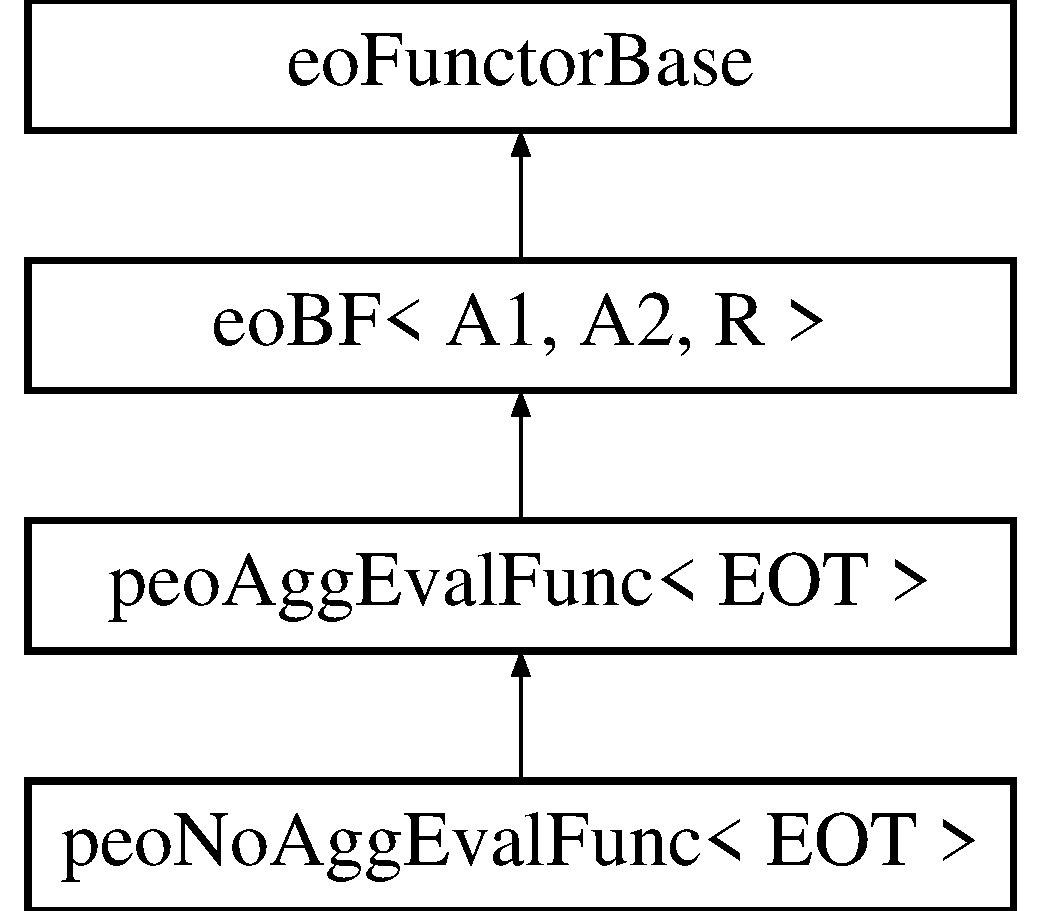
\includegraphics[height=4cm]{classpeoNoAggEvalFunc}
\end{center}
\end{figure}
\subsection*{Public Member Functions}
\begin{CompactItemize}
\item 
\hypertarget{classpeoNoAggEvalFunc_1a69ee1af8745ac75c864bf884436de5}{
void \hyperlink{classpeoNoAggEvalFunc_1a69ee1af8745ac75c864bf884436de5}{operator()} (EOT \&\_\-\_\-sol, const typename EOT::Fitness \&\_\-\_\-fit)}
\label{classpeoNoAggEvalFunc_1a69ee1af8745ac75c864bf884436de5}

\begin{CompactList}\small\item\em Operator which sets as fitness the {\bf \_\-\_\-fit} value for the {\bf \_\-\_\-sol} individual. \item\end{CompactList}\end{CompactItemize}


\subsection{Detailed Description}
\subsubsection*{template$<$class EOT$>$ class peo\-No\-Agg\-Eval\-Func$<$ EOT $>$}

The \hyperlink{classpeoNoAggEvalFunc}{peo\-No\-Agg\-Eval\-Func} class does nothing more than an association between a fitness value and a specified individual. 

The class is provided as a mean of declaring that no aggregation is required for the evaluation function - the fitness value is explicitly specified. 



Definition at line 47 of file peo\-No\-Agg\-Eval\-Func.h.

The documentation for this class was generated from the following file:\begin{CompactItemize}
\item 
peo\-No\-Agg\-Eval\-Func.h\end{CompactItemize}

\hypertarget{classpeoPopEval}{
\section{peo\-Pop\-Eval$<$ EOT $>$ Class Template Reference}
\label{classpeoPopEval}\index{peoPopEval@{peoPopEval}}
}
The {\bf \hyperlink{classpeoPopEval}{peo\-Pop\-Eval}} class provides the interface for constructing Paradis\-EO specific evaluation functors.  


{\tt \#include $<$peo\-Pop\-Eval.h$>$}

Inheritance diagram for peo\-Pop\-Eval$<$ EOT $>$::\begin{figure}[H]
\begin{center}
\leavevmode
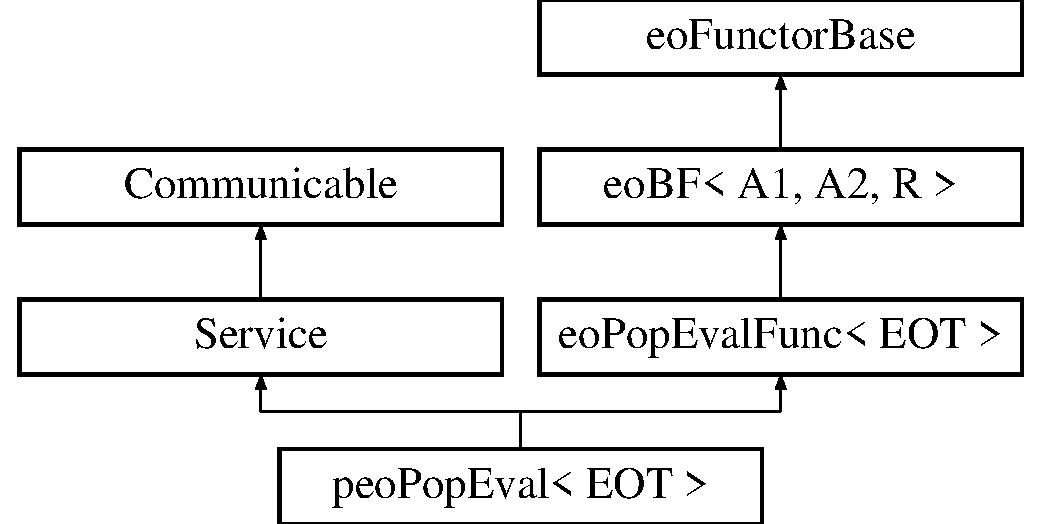
\includegraphics[height=4cm]{classpeoPopEval}
\end{center}
\end{figure}
\subsection*{Public Member Functions}
\begin{CompactItemize}
\item 
\hypertarget{classpeoPopEval_2f208067a5e39c3b26c1234050a41e8f}{
virtual void \hyperlink{classpeoPopEval_2f208067a5e39c3b26c1234050a41e8f}{operator()} (eo\-Pop$<$ EOT $>$ \&\_\-\_\-pop)=0}
\label{classpeoPopEval_2f208067a5e39c3b26c1234050a41e8f}

\begin{CompactList}\small\item\em Interface function providing the signature for constructing an evaluation functor. \item\end{CompactList}\end{CompactItemize}


\subsection{Detailed Description}
\subsubsection*{template$<$class EOT$>$ class peo\-Pop\-Eval$<$ EOT $>$}

The {\bf \hyperlink{classpeoPopEval}{peo\-Pop\-Eval}} class provides the interface for constructing Paradis\-EO specific evaluation functors. 

The derived classes may be used as wrappers for {\bf EO}-derived evaluation functors. In order to have an example, please refer to the implementation of the {\bf \hyperlink{classpeoSeqPopEval}{peo\-Seq\-Pop\-Eval}} and {\bf \hyperlink{classpeoParaPopEval}{peo\-Para\-Pop\-Eval}} classes. 



Definition at line 34 of file peo\-Pop\-Eval.h.

The documentation for this class was generated from the following file:\begin{CompactItemize}
\item 
peo\-Pop\-Eval.h\end{CompactItemize}

\hypertarget{classpeoPSOSelect}{
\section{peo\-PSOSelect$<$ POT $>$ Class Template Reference}
\label{classpeoPSOSelect}\index{peoPSOSelect@{peoPSOSelect}}
}
Specific class for a selection of a population of a PSO.  


{\tt \#include $<$peo\-PSO.h$>$}

Inheritance diagram for peo\-PSOSelect$<$ POT $>$::\begin{figure}[H]
\begin{center}
\leavevmode
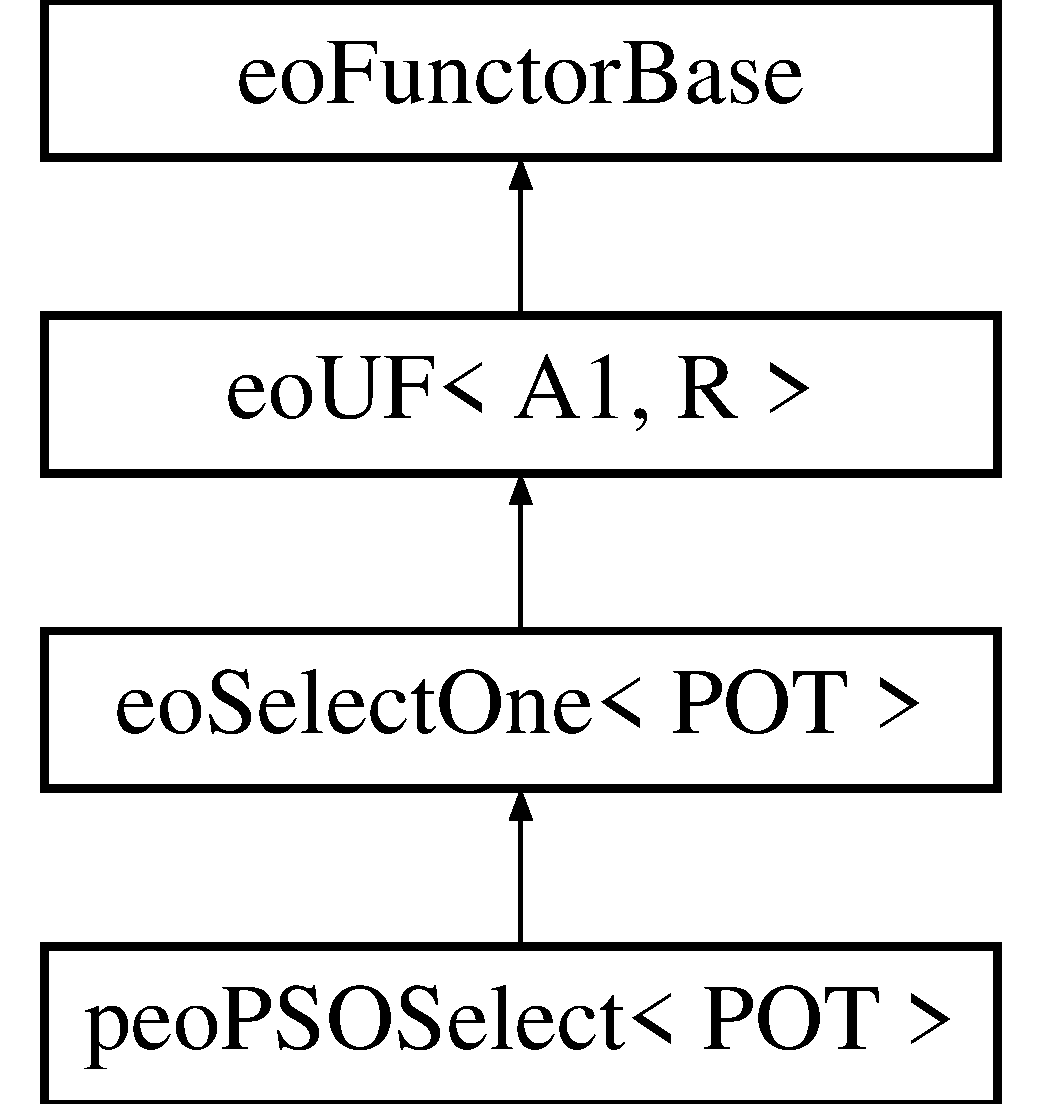
\includegraphics[height=4cm]{classpeoPSOSelect}
\end{center}
\end{figure}
\subsection*{Public Types}
\begin{CompactItemize}
\item 
\hypertarget{classpeoPSOSelect_6c39572e15b9236cd96bb9a306aacfa7}{
typedef \bf{PO}$<$ POT $>$::\hyperlink{classpeoPSOSelect_6c39572e15b9236cd96bb9a306aacfa7}{Fitness} \hyperlink{classpeoPSOSelect_6c39572e15b9236cd96bb9a306aacfa7}{Fitness}}
\label{classpeoPSOSelect_6c39572e15b9236cd96bb9a306aacfa7}

\begin{CompactList}\small\item\em typedef : creation of Fitness \item\end{CompactList}\end{CompactItemize}
\subsection*{Public Member Functions}
\begin{CompactItemize}
\item 
\hyperlink{classpeoPSOSelect_28c6552766e7ac08d2697a5c69c9b671}{peo\-PSOSelect} (\bf{eo\-Topology}$<$ POT $>$ \&\_\-topology)
\begin{CompactList}\small\item\em Constructor. \item\end{CompactList}\item 
virtual const POT \& \hyperlink{classpeoPSOSelect_13484074385f8896545dcbc72ba56d1c}{operator()} (const \bf{eo\-Pop}$<$ POT $>$ \&\_\-pop)
\begin{CompactList}\small\item\em Virtual operator. \item\end{CompactList}\end{CompactItemize}
\subsection*{Private Attributes}
\begin{CompactItemize}
\item 
\bf{eo\-Topology}$<$ POT $>$ \& \hyperlink{classpeoPSOSelect_8df48e9e116babf3010b618b61dfbeaf}{topology}
\end{CompactItemize}


\subsection{Detailed Description}
\subsubsection*{template$<$class POT$>$ class peo\-PSOSelect$<$ POT $>$}

Specific class for a selection of a population of a PSO. 

\begin{Desc}
\item[See also:]\doxyref{eo\-Select\-One} \end{Desc}
\begin{Desc}
\item[Version:]1.1 \end{Desc}
\begin{Desc}
\item[Date:]october 2007 \end{Desc}




Definition at line 54 of file peo\-PSO.h.

\subsection{Constructor \& Destructor Documentation}
\hypertarget{classpeoPSOSelect_28c6552766e7ac08d2697a5c69c9b671}{
\index{peoPSOSelect@{peo\-PSOSelect}!peoPSOSelect@{peoPSOSelect}}
\index{peoPSOSelect@{peoPSOSelect}!peoPSOSelect@{peo\-PSOSelect}}
\subsubsection[peoPSOSelect]{\setlength{\rightskip}{0pt plus 5cm}template$<$class POT$>$ \hyperlink{classpeoPSOSelect}{peo\-PSOSelect}$<$ POT $>$::\hyperlink{classpeoPSOSelect}{peo\-PSOSelect} (\bf{eo\-Topology}$<$ POT $>$ \& {\em \_\-topology})\hspace{0.3cm}{\tt  \mbox{[}inline\mbox{]}}}}
\label{classpeoPSOSelect_28c6552766e7ac08d2697a5c69c9b671}


Constructor. 

\begin{Desc}
\item[Parameters:]
\begin{description}
\item[{\em \doxyref{eo\-Topology}}]$<$ POT $>$ \& \_\-topology \end{description}
\end{Desc}


Definition at line 60 of file peo\-PSO.h.

\subsection{Member Function Documentation}
\hypertarget{classpeoPSOSelect_13484074385f8896545dcbc72ba56d1c}{
\index{peoPSOSelect@{peo\-PSOSelect}!operator()@{operator()}}
\index{operator()@{operator()}!peoPSOSelect@{peo\-PSOSelect}}
\subsubsection[operator()]{\setlength{\rightskip}{0pt plus 5cm}template$<$class POT$>$ virtual const POT\& \hyperlink{classpeoPSOSelect}{peo\-PSOSelect}$<$ POT $>$::operator() (const \bf{eo\-Pop}$<$ POT $>$ \& {\em \_\-pop})\hspace{0.3cm}{\tt  \mbox{[}inline, virtual\mbox{]}}}}
\label{classpeoPSOSelect_13484074385f8896545dcbc72ba56d1c}


Virtual operator. 

\begin{Desc}
\item[Parameters:]
\begin{description}
\item[{\em eo\-Pop$<$POT$>$\&}]\_\-pop \end{description}
\end{Desc}
\begin{Desc}
\item[Returns:]POT\& \end{Desc}


Definition at line 69 of file peo\-PSO.h.

References peo\-PSOSelect$<$ POT $>$::topology.

\subsection{Member Data Documentation}
\hypertarget{classpeoPSOSelect_8df48e9e116babf3010b618b61dfbeaf}{
\index{peoPSOSelect@{peo\-PSOSelect}!topology@{topology}}
\index{topology@{topology}!peoPSOSelect@{peo\-PSOSelect}}
\subsubsection[topology]{\setlength{\rightskip}{0pt plus 5cm}template$<$class POT$>$ \bf{eo\-Topology}$<$ POT $>$\& \hyperlink{classpeoPSOSelect}{peo\-PSOSelect}$<$ POT $>$::\hyperlink{classpeoPSOSelect_8df48e9e116babf3010b618b61dfbeaf}{topology}\hspace{0.3cm}{\tt  \mbox{[}private\mbox{]}}}}
\label{classpeoPSOSelect_8df48e9e116babf3010b618b61dfbeaf}


\begin{Desc}
\item[Parameters:]
\begin{description}
\item[{\em \doxyref{eo\-Topology}}]$<$ POT $>$ \& topology \end{description}
\end{Desc}


Definition at line 76 of file peo\-PSO.h.

Referenced by peo\-PSOSelect$<$ POT $>$::operator()().

The documentation for this class was generated from the following file:\begin{CompactItemize}
\item 
peo\-PSO.h\end{CompactItemize}

\hypertarget{classpeoSyncIslandMig}{
\section{peo\-Sync\-Island\-Mig$<$ TYPESELECT, TYPEREPLACE $>$ Class Template Reference}
\label{classpeoSyncIslandMig}\index{peoSyncIslandMig@{peoSyncIslandMig}}
}
Specific class for a synchronous migration.  


{\tt \#include $<$peo\-Sync\-Island\-Mig.h$>$}

Inheritance diagram for peo\-Sync\-Island\-Mig$<$ TYPESELECT, TYPEREPLACE $>$::\begin{figure}[H]
\begin{center}
\leavevmode
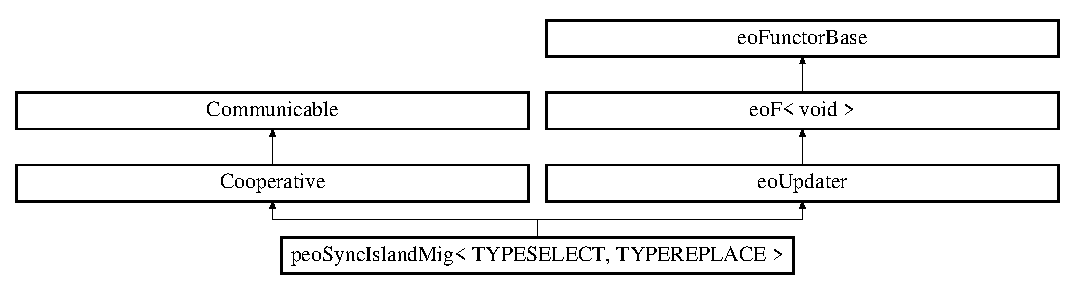
\includegraphics[height=3.44615cm]{classpeoSyncIslandMig}
\end{center}
\end{figure}
\subsection*{Public Member Functions}
\begin{CompactItemize}
\item 
\hyperlink{classpeoSyncIslandMig_24f4d1ea8bb63c09b9d6cd8476014082}{peo\-Sync\-Island\-Mig} (unsigned \_\-\_\-frequency, \hyperlink{classselector}{selector}$<$ TYPESELECT $>$ \&\_\-\_\-select, \hyperlink{classreplacement}{replacement}$<$ TYPEREPLACE $>$ \&\_\-\_\-replace, \hyperlink{classTopology}{Topology} \&\_\-\_\-topology)
\item 
\hypertarget{classpeoSyncIslandMig_0fd5b3b4e467ee33ae0186c0ae9d58ef}{
void \hyperlink{classpeoSyncIslandMig_0fd5b3b4e467ee33ae0186c0ae9d58ef}{operator()} ()}
\label{classpeoSyncIslandMig_0fd5b3b4e467ee33ae0186c0ae9d58ef}

\begin{CompactList}\small\item\em operator \item\end{CompactList}\item 
\hypertarget{classpeoSyncIslandMig_2daadf9928b8075ea469ca3cc49ddc88}{
void \hyperlink{classpeoSyncIslandMig_2daadf9928b8075ea469ca3cc49ddc88}{pack} ()}
\label{classpeoSyncIslandMig_2daadf9928b8075ea469ca3cc49ddc88}

\begin{CompactList}\small\item\em \doxyref{Function} realizing packages. \item\end{CompactList}\item 
\hypertarget{classpeoSyncIslandMig_25bc1a03cc49e17dda34b6647df1f9c5}{
void \hyperlink{classpeoSyncIslandMig_25bc1a03cc49e17dda34b6647df1f9c5}{unpack} ()}
\label{classpeoSyncIslandMig_25bc1a03cc49e17dda34b6647df1f9c5}

\begin{CompactList}\small\item\em \doxyref{Function} reconstituting packages. \item\end{CompactList}\item 
\hypertarget{classpeoSyncIslandMig_956f56110bccff8c8fae4b05aa804d32}{
void \hyperlink{classpeoSyncIslandMig_956f56110bccff8c8fae4b05aa804d32}{pack\-Synchronize\-Req} ()}
\label{classpeoSyncIslandMig_956f56110bccff8c8fae4b05aa804d32}

\begin{CompactList}\small\item\em \doxyref{Function} pack\-Synchronize\-Req. \item\end{CompactList}\item 
\hypertarget{classpeoSyncIslandMig_5f403428cea887b07caf27ab265ebe03}{
void \hyperlink{classpeoSyncIslandMig_5f403428cea887b07caf27ab265ebe03}{notify\-Sending} ()}
\label{classpeoSyncIslandMig_5f403428cea887b07caf27ab265ebe03}

\begin{CompactList}\small\item\em \doxyref{Function} notify\-Sending. \item\end{CompactList}\item 
\hypertarget{classpeoSyncIslandMig_75aacd3f7ffbc302c69addc342f45b8f}{
void \hyperlink{classpeoSyncIslandMig_75aacd3f7ffbc302c69addc342f45b8f}{notify\-Receiving} ()}
\label{classpeoSyncIslandMig_75aacd3f7ffbc302c69addc342f45b8f}

\begin{CompactList}\small\item\em \doxyref{Function} notify\-Receiving. \item\end{CompactList}\item 
\hypertarget{classpeoSyncIslandMig_92fef53496f935fe450589f90aec7d72}{
void \hyperlink{classpeoSyncIslandMig_92fef53496f935fe450589f90aec7d72}{notify\-Sending\-Sync\-Req} ()}
\label{classpeoSyncIslandMig_92fef53496f935fe450589f90aec7d72}

\begin{CompactList}\small\item\em notify\-Sending\-Sync\-Req \item\end{CompactList}\item 
\hypertarget{classpeoSyncIslandMig_0abd0c5872195cea0cab4988f9a4ea4e}{
void \hyperlink{classpeoSyncIslandMig_0abd0c5872195cea0cab4988f9a4ea4e}{notify\-Synchronized} ()}
\label{classpeoSyncIslandMig_0abd0c5872195cea0cab4988f9a4ea4e}

\begin{CompactList}\small\item\em notify\-Synchronized \item\end{CompactList}\end{CompactItemize}
\subsection*{Private Member Functions}
\begin{CompactItemize}
\item 
\hypertarget{classpeoSyncIslandMig_3ab202cb311f67fdc827078b3bdfddf4}{
void \hyperlink{classpeoSyncIslandMig_3ab202cb311f67fdc827078b3bdfddf4}{emigrate} ()}
\label{classpeoSyncIslandMig_3ab202cb311f67fdc827078b3bdfddf4}

\item 
\hypertarget{classpeoSyncIslandMig_baed2215bf06f96aacf06b5abff79f28}{
void \hyperlink{classpeoSyncIslandMig_baed2215bf06f96aacf06b5abff79f28}{immigrate} ()}
\label{classpeoSyncIslandMig_baed2215bf06f96aacf06b5abff79f28}

\end{CompactItemize}
\subsection*{Private Attributes}
\begin{CompactItemize}
\item 
\hyperlink{classeoSyncContinue}{eo\-Sync\-Continue} \hyperlink{classpeoSyncIslandMig_a64e7c9da149773c5d264d128a1ea37a}{cont}
\item 
\hypertarget{classpeoSyncIslandMig_a399c2533598dc8018eb2ab2edabd6b9}{
\hyperlink{classselector}{selector}$<$ TYPESELECT $>$ \& \hyperlink{classpeoSyncIslandMig_a399c2533598dc8018eb2ab2edabd6b9}{select}}
\label{classpeoSyncIslandMig_a399c2533598dc8018eb2ab2edabd6b9}

\item 
\hypertarget{classpeoSyncIslandMig_34b69e0a2fa12ef0f6101c7d04ebc3ef}{
\hyperlink{classreplacement}{replacement}$<$ TYPEREPLACE $>$ \& \hyperlink{classpeoSyncIslandMig_34b69e0a2fa12ef0f6101c7d04ebc3ef}{replace}}
\label{classpeoSyncIslandMig_34b69e0a2fa12ef0f6101c7d04ebc3ef}

\item 
\hypertarget{classpeoSyncIslandMig_7376532c3a8bcab88a02601611db9f2f}{
\hyperlink{classTopology}{Topology} \& \hyperlink{classpeoSyncIslandMig_7376532c3a8bcab88a02601611db9f2f}{topology}}
\label{classpeoSyncIslandMig_7376532c3a8bcab88a02601611db9f2f}

\item 
\hypertarget{classpeoSyncIslandMig_4c734df065099cfd5693d35fae38ad29}{
std::queue$<$ TYPEREPLACE $>$ \hyperlink{classpeoSyncIslandMig_4c734df065099cfd5693d35fae38ad29}{imm}}
\label{classpeoSyncIslandMig_4c734df065099cfd5693d35fae38ad29}

\item 
\hypertarget{classpeoSyncIslandMig_b96f8caff26498798eb0e4c114ee5d9a}{
std::queue$<$ TYPESELECT $>$ \hyperlink{classpeoSyncIslandMig_b96f8caff26498798eb0e4c114ee5d9a}{em}}
\label{classpeoSyncIslandMig_b96f8caff26498798eb0e4c114ee5d9a}

\item 
\hypertarget{classpeoSyncIslandMig_ad56e3475d8ea7a83007c2e32c7da6a8}{
std::queue$<$ \hyperlink{classCooperative}{Cooperative} $\ast$ $>$ \hyperlink{classpeoSyncIslandMig_ad56e3475d8ea7a83007c2e32c7da6a8}{coop\_\-em}}
\label{classpeoSyncIslandMig_ad56e3475d8ea7a83007c2e32c7da6a8}

\item 
\hypertarget{classpeoSyncIslandMig_9431b7e1d629f238cd5f990d02926480}{
sem\_\-t \hyperlink{classpeoSyncIslandMig_9431b7e1d629f238cd5f990d02926480}{sync}}
\label{classpeoSyncIslandMig_9431b7e1d629f238cd5f990d02926480}

\item 
\hypertarget{classpeoSyncIslandMig_253dfbfebfadad0b4f49e60bb811b1db}{
bool \hyperlink{classpeoSyncIslandMig_253dfbfebfadad0b4f49e60bb811b1db}{explicit\-Passive}}
\label{classpeoSyncIslandMig_253dfbfebfadad0b4f49e60bb811b1db}

\item 
\hypertarget{classpeoSyncIslandMig_e5d64ff9718b746d2307379fb061ad96}{
bool \hyperlink{classpeoSyncIslandMig_e5d64ff9718b746d2307379fb061ad96}{standby\-Migration}}
\label{classpeoSyncIslandMig_e5d64ff9718b746d2307379fb061ad96}

\item 
\hypertarget{classpeoSyncIslandMig_6274e5185b6b7579dea71da3138d9d23}{
std::vector$<$ \hyperlink{classCooperative}{Cooperative} $\ast$ $>$ \hyperlink{classpeoSyncIslandMig_6274e5185b6b7579dea71da3138d9d23}{in}}
\label{classpeoSyncIslandMig_6274e5185b6b7579dea71da3138d9d23}

\item 
\hypertarget{classpeoSyncIslandMig_daae2fea2f447d35927e18a8f008a45d}{
std::vector$<$ \hyperlink{classCooperative}{Cooperative} $\ast$ $>$ \hyperlink{classpeoSyncIslandMig_daae2fea2f447d35927e18a8f008a45d}{out}}
\label{classpeoSyncIslandMig_daae2fea2f447d35927e18a8f008a45d}

\item 
\hypertarget{classpeoSyncIslandMig_2760dde833d7141ca86affb4df0fb163}{
std::vector$<$ \hyperlink{classCooperative}{Cooperative} $\ast$ $>$ \hyperlink{classpeoSyncIslandMig_2760dde833d7141ca86affb4df0fb163}{all}}
\label{classpeoSyncIslandMig_2760dde833d7141ca86affb4df0fb163}

\item 
\hypertarget{classpeoSyncIslandMig_cdd55a0ab14d659a2a68674a05ed8a1d}{
unsigned \hyperlink{classpeoSyncIslandMig_cdd55a0ab14d659a2a68674a05ed8a1d}{nb\-Migrations}}
\label{classpeoSyncIslandMig_cdd55a0ab14d659a2a68674a05ed8a1d}

\end{CompactItemize}


\subsection{Detailed Description}
\subsubsection*{template$<$class TYPESELECT, class TYPEREPLACE$>$ class peo\-Sync\-Island\-Mig$<$ TYPESELECT, TYPEREPLACE $>$}

Specific class for a synchronous migration. 

\begin{Desc}
\item[See also:]\hyperlink{classCooperative}{Cooperative} \doxyref{eo\-Updater} \end{Desc}
\begin{Desc}
\item[Version:]2.0 \end{Desc}
\begin{Desc}
\item[Date:]january 2008 \end{Desc}




Definition at line 71 of file peo\-Sync\-Island\-Mig.h.

\subsection{Constructor \& Destructor Documentation}
\hypertarget{classpeoSyncIslandMig_24f4d1ea8bb63c09b9d6cd8476014082}{
\index{peoSyncIslandMig@{peo\-Sync\-Island\-Mig}!peoSyncIslandMig@{peoSyncIslandMig}}
\index{peoSyncIslandMig@{peoSyncIslandMig}!peoSyncIslandMig@{peo\-Sync\-Island\-Mig}}
\subsubsection[peoSyncIslandMig]{\setlength{\rightskip}{0pt plus 5cm}template$<$class TYPESELECT, class TYPEREPLACE$>$ \hyperlink{classpeoSyncIslandMig}{peo\-Sync\-Island\-Mig}$<$ TYPESELECT, TYPEREPLACE $>$::\hyperlink{classpeoSyncIslandMig}{peo\-Sync\-Island\-Mig} (unsigned {\em \_\-\_\-frequency}, \hyperlink{classselector}{selector}$<$ TYPESELECT $>$ \& {\em \_\-\_\-select}, \hyperlink{classreplacement}{replacement}$<$ TYPEREPLACE $>$ \& {\em \_\-\_\-replace}, \hyperlink{classTopology}{Topology} \& {\em \_\-\_\-topology})}}
\label{classpeoSyncIslandMig_24f4d1ea8bb63c09b9d6cd8476014082}


\begin{Desc}
\item[Parameters:]
\begin{description}
\item[{\em unsigned}]\_\-\_\-frequency \item[{\em selector}]$<$TYPESELECT$>$ \& \_\-\_\-select \item[{\em replacement}]$<$TYPEREPLACE$>$ \& \_\-\_\-replace \item[{\em Topology\&}]\_\-\_\-topology \end{description}
\end{Desc}


Definition at line 139 of file peo\-Sync\-Island\-Mig.h.

References Topology::add(), and peo\-Sync\-Island\-Mig$<$ TYPESELECT, TYPEREPLACE $>$::sync.

\subsection{Member Data Documentation}
\hypertarget{classpeoSyncIslandMig_a64e7c9da149773c5d264d128a1ea37a}{
\index{peoSyncIslandMig@{peo\-Sync\-Island\-Mig}!cont@{cont}}
\index{cont@{cont}!peoSyncIslandMig@{peo\-Sync\-Island\-Mig}}
\subsubsection[cont]{\setlength{\rightskip}{0pt plus 5cm}template$<$class TYPESELECT, class TYPEREPLACE$>$ \hyperlink{classeoSyncContinue}{eo\-Sync\-Continue} \hyperlink{classpeoSyncIslandMig}{peo\-Sync\-Island\-Mig}$<$ TYPESELECT, TYPEREPLACE $>$::\hyperlink{classpeoSyncIslandMig_a64e7c9da149773c5d264d128a1ea37a}{cont}\hspace{0.3cm}{\tt  \mbox{[}private\mbox{]}}}}
\label{classpeoSyncIslandMig_a64e7c9da149773c5d264d128a1ea37a}


\begin{Desc}
\item[Parameters:]
\begin{description}
\item[{\em \hyperlink{classeoSyncContinue}{eo\-Sync\-Continue}}]cont \item[{\em selector}]$<$TYPESELECT$>$ \& select \item[{\em replacement}]$<$TYPEREPLACE$>$ \& replace \item[{\em Topology\&}]topology \item[{\em std}]:: queue$<$ TYPEREPLACE $>$ imm \item[{\em std}]:: queue$<$ TYPESELECT $>$ em \item[{\em std}]:: queue$<$ Cooperative$\ast$ $>$ coop\_\-em \item[{\em sem\_\-t}]sync \item[{\em bool}]explicit\-Passive \item[{\em bool}]standby\-Migration \item[{\em std}]:: vector$<$ Cooperative$\ast$ $>$ in, out, all \item[{\em unsigned}]nb\-Migrations \end{description}
\end{Desc}


Definition at line 124 of file peo\-Sync\-Island\-Mig.h.

Referenced by peo\-Sync\-Island\-Mig$<$ TYPESELECT, TYPEREPLACE $>$::operator()().

The documentation for this class was generated from the following file:\begin{CompactItemize}
\item 
peo\-Sync\-Island\-Mig.h\end{CompactItemize}

\hypertarget{classpeoTransform}{
\section{peo\-Transform$<$ EOT $>$ Class Template Reference}
\label{classpeoTransform}\index{peoTransform@{peoTransform}}
}
The \hyperlink{classpeoTransform}{peo\-Transform} class acts only as an interface for creating transform operators - for an example please refer to the {\bf \hyperlink{classpeoSeqTransform}{peo\-Seq\-Transform}} and the {\bf \hyperlink{classpeoParaSGATransform}{peo\-Para\-SGATransform}} classes.  


{\tt \#include $<$peo\-Transform.h$>$}

Inheritance diagram for peo\-Transform$<$ EOT $>$::\begin{figure}[H]
\begin{center}
\leavevmode
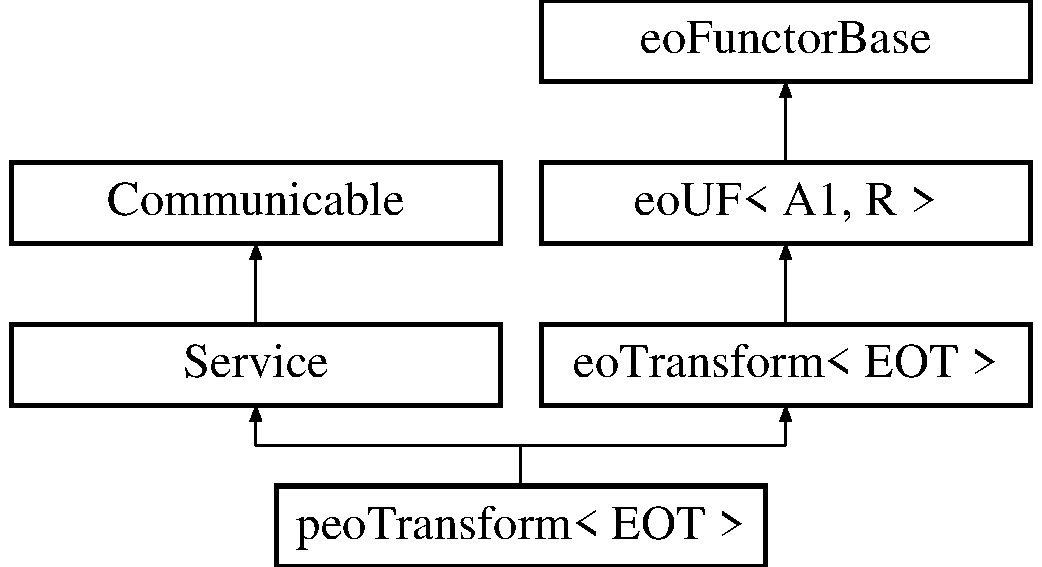
\includegraphics[height=4cm]{classpeoTransform}
\end{center}
\end{figure}


\subsection{Detailed Description}
\subsubsection*{template$<$class EOT$>$ class peo\-Transform$<$ EOT $>$}

The \hyperlink{classpeoTransform}{peo\-Transform} class acts only as an interface for creating transform operators - for an example please refer to the {\bf \hyperlink{classpeoSeqTransform}{peo\-Seq\-Transform}} and the {\bf \hyperlink{classpeoParaSGATransform}{peo\-Para\-SGATransform}} classes. 



Definition at line 20 of file peo\-Transform.h.

The documentation for this class was generated from the following file:\begin{CompactItemize}
\item 
peo\-Transform.h\end{CompactItemize}

\hypertarget{classpeoWorstPositionReplacement}{
\section{peo\-Worst\-Position\-Replacement$<$ POT $>$ Class Template Reference}
\label{classpeoWorstPositionReplacement}\index{peoWorstPositionReplacement@{peoWorstPositionReplacement}}
}
Specific class for a replacement of a population of a PSO.  


{\tt \#include $<$peo\-PSO.h$>$}

Inheritance diagram for peo\-Worst\-Position\-Replacement$<$ POT $>$::\begin{figure}[H]
\begin{center}
\leavevmode
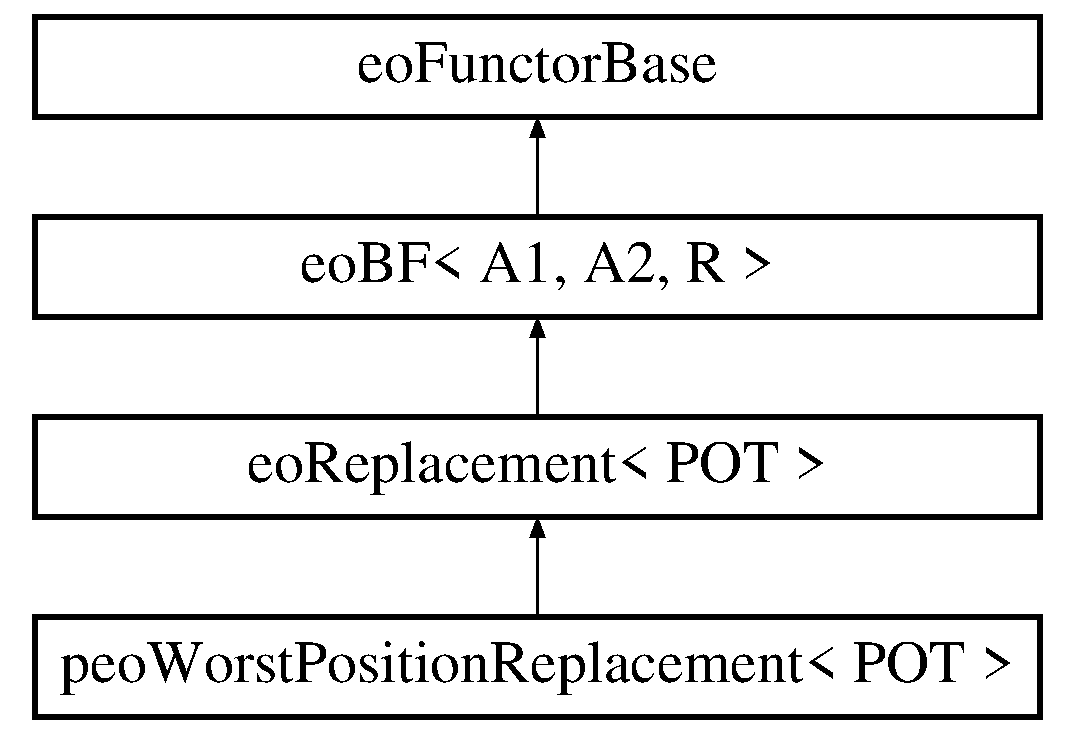
\includegraphics[height=4cm]{classpeoWorstPositionReplacement}
\end{center}
\end{figure}
\subsection*{Public Member Functions}
\begin{CompactItemize}
\item 
\hypertarget{classpeoWorstPositionReplacement_8d6eeb59dbcf71e681a122e2650901f8}{
\hyperlink{classpeoWorstPositionReplacement_8d6eeb59dbcf71e681a122e2650901f8}{peo\-Worst\-Position\-Replacement} ()}
\label{classpeoWorstPositionReplacement_8d6eeb59dbcf71e681a122e2650901f8}

\begin{CompactList}\small\item\em constructor \item\end{CompactList}\item 
void \hyperlink{classpeoWorstPositionReplacement_3771416291c82aca15f9175f36552669}{operator()} (\bf{eo\-Pop}$<$ POT $>$ \&\_\-dest, \bf{eo\-Pop}$<$ POT $>$ \&\_\-source)
\begin{CompactList}\small\item\em operator \item\end{CompactList}\end{CompactItemize}


\subsection{Detailed Description}
\subsubsection*{template$<$class POT$>$ class peo\-Worst\-Position\-Replacement$<$ POT $>$}

Specific class for a replacement of a population of a PSO. 

\begin{Desc}
\item[See also:]\doxyref{eo\-Replacement} \end{Desc}
\begin{Desc}
\item[Version:]1.1 \end{Desc}
\begin{Desc}
\item[Date:]october 2007 \end{Desc}




Definition at line 127 of file peo\-PSO.h.

\subsection{Member Function Documentation}
\hypertarget{classpeoWorstPositionReplacement_3771416291c82aca15f9175f36552669}{
\index{peoWorstPositionReplacement@{peo\-Worst\-Position\-Replacement}!operator()@{operator()}}
\index{operator()@{operator()}!peoWorstPositionReplacement@{peo\-Worst\-Position\-Replacement}}
\subsubsection[operator()]{\setlength{\rightskip}{0pt plus 5cm}template$<$class POT$>$ void \hyperlink{classpeoWorstPositionReplacement}{peo\-Worst\-Position\-Replacement}$<$ POT $>$::operator() (\bf{eo\-Pop}$<$ POT $>$ \& {\em \_\-dest}, \bf{eo\-Pop}$<$ POT $>$ \& {\em \_\-source})\hspace{0.3cm}{\tt  \mbox{[}inline\mbox{]}}}}
\label{classpeoWorstPositionReplacement_3771416291c82aca15f9175f36552669}


operator 

\begin{Desc}
\item[Parameters:]
\begin{description}
\item[{\em eo\-Pop$<$POT$>$\&}]\_\-dest \item[{\em eo\-Pop$<$POT$>$\&}]\_\-source \end{description}
\end{Desc}


Definition at line 137 of file peo\-PSO.h.

The documentation for this class was generated from the following file:\begin{CompactItemize}
\item 
peo\-PSO.h\end{CompactItemize}

\hypertarget{classpeoWrapper}{
\section{peo\-Wrapper Class Reference}
\label{classpeoWrapper}\index{peoWrapper@{peoWrapper}}
}
Specific class for wrapping.  


{\tt \#include $<$peo\-Wrapper.h$>$}

Inheritance diagram for peo\-Wrapper::\begin{figure}[H]
\begin{center}
\leavevmode
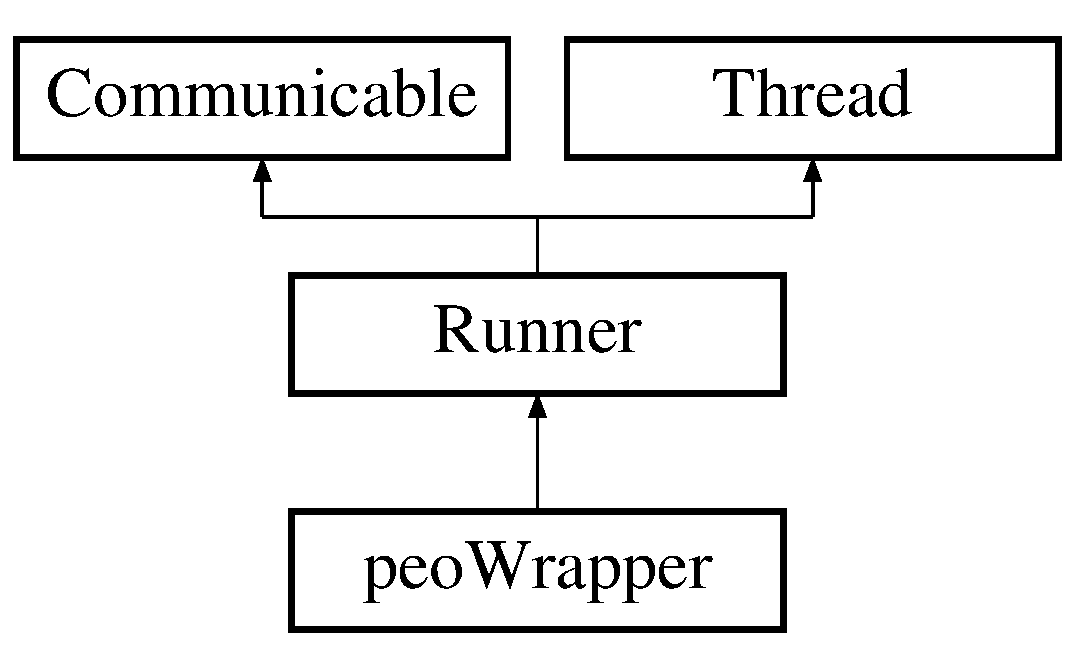
\includegraphics[height=3cm]{classpeoWrapper}
\end{center}
\end{figure}
\subsection*{Public Member Functions}
\begin{CompactItemize}
\item 
template$<$typename Algorithm\-Type$>$ \hyperlink{classpeoWrapper_b0a651003934a41269db4b9f09696b7b}{peo\-Wrapper} (Algorithm\-Type \&external\-Algorithm)
\begin{CompactList}\small\item\em constructor \item\end{CompactList}\item 
template$<$typename Algorithm\-Type, typename Algorithm\-Data\-Type$>$ \hyperlink{classpeoWrapper_f995a4006a82472f3465b079ae303a57}{peo\-Wrapper} (Algorithm\-Type \&external\-Algorithm, Algorithm\-Data\-Type \&external\-Data)
\begin{CompactList}\small\item\em constructor \item\end{CompactList}\item 
template$<$typename Algorithm\-Return\-Type$>$ \hyperlink{classpeoWrapper_593608a5637ba48e0cc3471f093b42bb}{peo\-Wrapper} (Algorithm\-Return\-Type \&($\ast$external\-Algorithm)())
\begin{CompactList}\small\item\em constructor \item\end{CompactList}\item 
template$<$typename Algorithm\-Return\-Type, typename Algorithm\-Data\-Type$>$ \hyperlink{classpeoWrapper_b4a2e26d0806791847db1695ec46cce1}{peo\-Wrapper} (Algorithm\-Return\-Type \&($\ast$external\-Algorithm)(Algorithm\-Data\-Type \&), Algorithm\-Data\-Type \&external\-Data)
\begin{CompactList}\small\item\em constructor \item\end{CompactList}\item 
\hypertarget{classpeoWrapper_756a0ee6b6b3edb98516e8eef707808c}{
\hyperlink{classpeoWrapper_756a0ee6b6b3edb98516e8eef707808c}{$\sim$peo\-Wrapper} ()}
\label{classpeoWrapper_756a0ee6b6b3edb98516e8eef707808c}

\begin{CompactList}\small\item\em destructor \item\end{CompactList}\item 
\hypertarget{classpeoWrapper_ed88d78762dcd6489ff725a4aa2b81a7}{
void \hyperlink{classpeoWrapper_ed88d78762dcd6489ff725a4aa2b81a7}{run} ()}
\label{classpeoWrapper_ed88d78762dcd6489ff725a4aa2b81a7}

\begin{CompactList}\small\item\em function run \item\end{CompactList}\end{CompactItemize}
\subsection*{Private Attributes}
\begin{CompactItemize}
\item 
\hyperlink{structpeoWrapper_1_1AbstractAlgorithm}{Abstract\-Algorithm} $\ast$ \hyperlink{classpeoWrapper_d191ac6d451db7aca86fed473b711346}{algorithm}
\end{CompactItemize}
\subsection*{Classes}
\begin{CompactItemize}
\item 
struct \hyperlink{structpeoWrapper_1_1AbstractAlgorithm}{Abstract\-Algorithm}
\item 
struct \hyperlink{structpeoWrapper_1_1Algorithm}{Algorithm}
\item 
struct \hyperlink{structpeoWrapper_1_1Algorithm_3_01AlgorithmType_00_01void_01_4}{Algorithm$<$ Algorithm\-Type, void $>$}
\item 
struct \hyperlink{structpeoWrapper_1_1FunctionAlgorithm}{Function\-Algorithm}
\item 
struct \hyperlink{structpeoWrapper_1_1FunctionAlgorithm_3_01AlgorithmReturnType_00_01void_01_4}{Function\-Algorithm$<$ Algorithm\-Return\-Type, void $>$}
\end{CompactItemize}


\subsection{Detailed Description}
Specific class for wrapping. 

\begin{Desc}
\item[See also:]\hyperlink{classRunner}{Runner} \end{Desc}
\begin{Desc}
\item[Version:]1.1 \end{Desc}
\begin{Desc}
\item[Date:]december 2007 \end{Desc}




Definition at line 49 of file peo\-Wrapper.h.

\subsection{Constructor \& Destructor Documentation}
\hypertarget{classpeoWrapper_b0a651003934a41269db4b9f09696b7b}{
\index{peoWrapper@{peo\-Wrapper}!peoWrapper@{peoWrapper}}
\index{peoWrapper@{peoWrapper}!peoWrapper@{peo\-Wrapper}}
\subsubsection[peoWrapper]{\setlength{\rightskip}{0pt plus 5cm}template$<$typename Algorithm\-Type$>$ peo\-Wrapper::peo\-Wrapper (Algorithm\-Type \& {\em external\-Algorithm})\hspace{0.3cm}{\tt  \mbox{[}inline\mbox{]}}}}
\label{classpeoWrapper_b0a651003934a41269db4b9f09696b7b}


constructor 

\begin{Desc}
\item[Parameters:]
\begin{description}
\item[{\em Algorithm\-Type\&}]external\-Algorithm \end{description}
\end{Desc}


Definition at line 56 of file peo\-Wrapper.h.\hypertarget{classpeoWrapper_f995a4006a82472f3465b079ae303a57}{
\index{peoWrapper@{peo\-Wrapper}!peoWrapper@{peoWrapper}}
\index{peoWrapper@{peoWrapper}!peoWrapper@{peo\-Wrapper}}
\subsubsection[peoWrapper]{\setlength{\rightskip}{0pt plus 5cm}template$<$typename Algorithm\-Type, typename Algorithm\-Data\-Type$>$ peo\-Wrapper::peo\-Wrapper (Algorithm\-Type \& {\em external\-Algorithm}, Algorithm\-Data\-Type \& {\em external\-Data})\hspace{0.3cm}{\tt  \mbox{[}inline\mbox{]}}}}
\label{classpeoWrapper_f995a4006a82472f3465b079ae303a57}


constructor 

\begin{Desc}
\item[Parameters:]
\begin{description}
\item[{\em Algorithm\-Type\&}]external\-Algorithm \item[{\em Algorithm\-Data\-Type\&}]external\-Data \end{description}
\end{Desc}


Definition at line 63 of file peo\-Wrapper.h.\hypertarget{classpeoWrapper_593608a5637ba48e0cc3471f093b42bb}{
\index{peoWrapper@{peo\-Wrapper}!peoWrapper@{peoWrapper}}
\index{peoWrapper@{peoWrapper}!peoWrapper@{peo\-Wrapper}}
\subsubsection[peoWrapper]{\setlength{\rightskip}{0pt plus 5cm}template$<$typename Algorithm\-Return\-Type$>$ peo\-Wrapper::peo\-Wrapper (Algorithm\-Return\-Type \&($\ast$)() {\em external\-Algorithm})\hspace{0.3cm}{\tt  \mbox{[}inline\mbox{]}}}}
\label{classpeoWrapper_593608a5637ba48e0cc3471f093b42bb}


constructor 

\begin{Desc}
\item[Parameters:]
\begin{description}
\item[{\em Algorithm\-Return\-Type\&}]($\ast$external\-Algorithm)() \end{description}
\end{Desc}


Definition at line 69 of file peo\-Wrapper.h.\hypertarget{classpeoWrapper_b4a2e26d0806791847db1695ec46cce1}{
\index{peoWrapper@{peo\-Wrapper}!peoWrapper@{peoWrapper}}
\index{peoWrapper@{peoWrapper}!peoWrapper@{peo\-Wrapper}}
\subsubsection[peoWrapper]{\setlength{\rightskip}{0pt plus 5cm}template$<$typename Algorithm\-Return\-Type, typename Algorithm\-Data\-Type$>$ peo\-Wrapper::peo\-Wrapper (Algorithm\-Return\-Type \&($\ast$)(Algorithm\-Data\-Type \&) {\em external\-Algorithm}, Algorithm\-Data\-Type \& {\em external\-Data})\hspace{0.3cm}{\tt  \mbox{[}inline\mbox{]}}}}
\label{classpeoWrapper_b4a2e26d0806791847db1695ec46cce1}


constructor 

\begin{Desc}
\item[Parameters:]
\begin{description}
\item[{\em Algorithm\-Return\-Type\&}]($\ast$external\-Algorithm)( Algorithm\-Data\-Type\& ) \item[{\em Algorithm\-Data\-Type\&}]external\-Data \end{description}
\end{Desc}


Definition at line 76 of file peo\-Wrapper.h.

\subsection{Member Data Documentation}
\hypertarget{classpeoWrapper_d191ac6d451db7aca86fed473b711346}{
\index{peoWrapper@{peo\-Wrapper}!algorithm@{algorithm}}
\index{algorithm@{algorithm}!peoWrapper@{peo\-Wrapper}}
\subsubsection[algorithm]{\setlength{\rightskip}{0pt plus 5cm}\hyperlink{structpeoWrapper_1_1AbstractAlgorithm}{Abstract\-Algorithm}$\ast$ \hyperlink{classpeoWrapper_d191ac6d451db7aca86fed473b711346}{peo\-Wrapper::algorithm}\hspace{0.3cm}{\tt  \mbox{[}private\mbox{]}}}}
\label{classpeoWrapper_d191ac6d451db7aca86fed473b711346}


\begin{Desc}
\item[Parameters:]
\begin{description}
\item[{\em Abstract\-Algorithm$\ast$}]algorithm \end{description}
\end{Desc}


Definition at line 170 of file peo\-Wrapper.h.

Referenced by run(), and $\sim$peo\-Wrapper().

The documentation for this class was generated from the following file:\begin{CompactItemize}
\item 
peo\-Wrapper.h\end{CompactItemize}

\hypertarget{structpeoWrapper_1_1AbstractAlgorithm}{
\section{peo\-Wrapper::Abstract\-Algorithm Struct Reference}
\label{structpeoWrapper_1_1AbstractAlgorithm}\index{peoWrapper::AbstractAlgorithm@{peoWrapper::AbstractAlgorithm}}
}
Inheritance diagram for peo\-Wrapper::Abstract\-Algorithm::\begin{figure}[H]
\begin{center}
\leavevmode
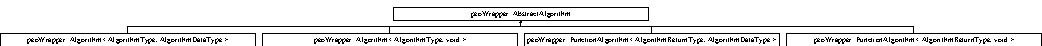
\includegraphics[height=0.614035cm]{structpeoWrapper_1_1AbstractAlgorithm}
\end{center}
\end{figure}
\subsection*{Public Member Functions}
\begin{CompactItemize}
\item 
\hypertarget{structpeoWrapper_1_1AbstractAlgorithm_30a579ba96072332f60989f92de669e9}{
virtual \hyperlink{structpeoWrapper_1_1AbstractAlgorithm_30a579ba96072332f60989f92de669e9}{$\sim$Abstract\-Algorithm} ()}
\label{structpeoWrapper_1_1AbstractAlgorithm_30a579ba96072332f60989f92de669e9}

\item 
\hypertarget{structpeoWrapper_1_1AbstractAlgorithm_a9aa8c613ea6c944b296cf3ba5f6f95b}{
virtual void \hyperlink{structpeoWrapper_1_1AbstractAlgorithm_a9aa8c613ea6c944b296cf3ba5f6f95b}{operator()} ()}
\label{structpeoWrapper_1_1AbstractAlgorithm_a9aa8c613ea6c944b296cf3ba5f6f95b}

\end{CompactItemize}


\subsection{Detailed Description}




Definition at line 95 of file peo\-Wrapper.h.

The documentation for this struct was generated from the following file:\begin{CompactItemize}
\item 
peo\-Wrapper.h\end{CompactItemize}

\hypertarget{structpeoWrapper_1_1Algorithm}{
\section{peo\-Wrapper::Algorithm$<$ Algorithm\-Type, Algorithm\-Data\-Type $>$ Struct Template Reference}
\label{structpeoWrapper_1_1Algorithm}\index{peoWrapper::Algorithm@{peoWrapper::Algorithm}}
}
Inheritance diagram for peo\-Wrapper::Algorithm$<$ Algorithm\-Type, Algorithm\-Data\-Type $>$::\begin{figure}[H]
\begin{center}
\leavevmode
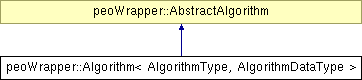
\includegraphics[height=2cm]{structpeoWrapper_1_1Algorithm}
\end{center}
\end{figure}
\subsection*{Public Member Functions}
\begin{CompactItemize}
\item 
\hypertarget{structpeoWrapper_1_1Algorithm_6b615c46939bba8ff8d1c7f35b5d47b8}{
\hyperlink{structpeoWrapper_1_1Algorithm_6b615c46939bba8ff8d1c7f35b5d47b8}{Algorithm} (Algorithm\-Type \&external\-Algorithm, Algorithm\-Data\-Type \&external\-Data)}
\label{structpeoWrapper_1_1Algorithm_6b615c46939bba8ff8d1c7f35b5d47b8}

\item 
\hypertarget{structpeoWrapper_1_1Algorithm_8db189b4456bcf056b327ecbf000de7b}{
virtual void \hyperlink{structpeoWrapper_1_1Algorithm_8db189b4456bcf056b327ecbf000de7b}{operator()} ()}
\label{structpeoWrapper_1_1Algorithm_8db189b4456bcf056b327ecbf000de7b}

\end{CompactItemize}
\subsection*{Public Attributes}
\begin{CompactItemize}
\item 
\hypertarget{structpeoWrapper_1_1Algorithm_eb826079a4c774ade1e933acbdd401c2}{
Algorithm\-Type \& \hyperlink{structpeoWrapper_1_1Algorithm_eb826079a4c774ade1e933acbdd401c2}{algorithm}}
\label{structpeoWrapper_1_1Algorithm_eb826079a4c774ade1e933acbdd401c2}

\item 
\hypertarget{structpeoWrapper_1_1Algorithm_2c9f577fe7519df7fda1f2afd08b7c91}{
Algorithm\-Data\-Type \& \hyperlink{structpeoWrapper_1_1Algorithm_2c9f577fe7519df7fda1f2afd08b7c91}{algorithm\-Data}}
\label{structpeoWrapper_1_1Algorithm_2c9f577fe7519df7fda1f2afd08b7c91}

\end{CompactItemize}


\subsection{Detailed Description}
\subsubsection*{template$<$typename Algorithm\-Type, typename Algorithm\-Data\-Type$>$ struct peo\-Wrapper::Algorithm$<$ Algorithm\-Type, Algorithm\-Data\-Type $>$}





Definition at line 107 of file peo\-Wrapper.h.

The documentation for this struct was generated from the following file:\begin{CompactItemize}
\item 
peo\-Wrapper.h\end{CompactItemize}

\hypertarget{structpeoWrapper_1_1Algorithm_3_01AlgorithmType_00_01void_01_4}{
\section{peo\-Wrapper::Algorithm$<$ Algorithm\-Type, void $>$ Struct Template Reference}
\label{structpeoWrapper_1_1Algorithm_3_01AlgorithmType_00_01void_01_4}\index{peoWrapper::Algorithm< AlgorithmType, void >@{peoWrapper::Algorithm$<$ AlgorithmType, void $>$}}
}
Inheritance diagram for peo\-Wrapper::Algorithm$<$ Algorithm\-Type, void $>$::\begin{figure}[H]
\begin{center}
\leavevmode
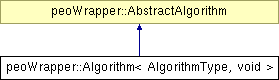
\includegraphics[height=2cm]{structpeoWrapper_1_1Algorithm_3_01AlgorithmType_00_01void_01_4}
\end{center}
\end{figure}
\subsection*{Public Member Functions}
\begin{CompactItemize}
\item 
\hypertarget{structpeoWrapper_1_1Algorithm_3_01AlgorithmType_00_01void_01_4_a1223438f15e954880a0a9833890dd91}{
\hyperlink{structpeoWrapper_1_1Algorithm_3_01AlgorithmType_00_01void_01_4_a1223438f15e954880a0a9833890dd91}{Algorithm} (Algorithm\-Type \&external\-Algorithm)}
\label{structpeoWrapper_1_1Algorithm_3_01AlgorithmType_00_01void_01_4_a1223438f15e954880a0a9833890dd91}

\item 
\hypertarget{structpeoWrapper_1_1Algorithm_3_01AlgorithmType_00_01void_01_4_c6fe207372bb3b53c7ccecf6d596c4e5}{
virtual void \hyperlink{structpeoWrapper_1_1Algorithm_3_01AlgorithmType_00_01void_01_4_c6fe207372bb3b53c7ccecf6d596c4e5}{operator()} ()}
\label{structpeoWrapper_1_1Algorithm_3_01AlgorithmType_00_01void_01_4_c6fe207372bb3b53c7ccecf6d596c4e5}

\end{CompactItemize}
\subsection*{Public Attributes}
\begin{CompactItemize}
\item 
\hypertarget{structpeoWrapper_1_1Algorithm_3_01AlgorithmType_00_01void_01_4_9be62964456f157d5cef10710905a314}{
Algorithm\-Type \& \hyperlink{structpeoWrapper_1_1Algorithm_3_01AlgorithmType_00_01void_01_4_9be62964456f157d5cef10710905a314}{algorithm}}
\label{structpeoWrapper_1_1Algorithm_3_01AlgorithmType_00_01void_01_4_9be62964456f157d5cef10710905a314}

\end{CompactItemize}


\subsection{Detailed Description}
\subsubsection*{template$<$typename Algorithm\-Type$>$ struct peo\-Wrapper::Algorithm$<$ Algorithm\-Type, void $>$}





Definition at line 123 of file peo\-Wrapper.h.

The documentation for this struct was generated from the following file:\begin{CompactItemize}
\item 
peo\-Wrapper.h\end{CompactItemize}

\hypertarget{structpeoWrapper_1_1FunctionAlgorithm}{
\section{peo\-Wrapper::Function\-Algorithm$<$ Algorithm\-Return\-Type, Algorithm\-Data\-Type $>$ Struct Template Reference}
\label{structpeoWrapper_1_1FunctionAlgorithm}\index{peoWrapper::FunctionAlgorithm@{peoWrapper::FunctionAlgorithm}}
}
Inheritance diagram for peo\-Wrapper::Function\-Algorithm$<$ Algorithm\-Return\-Type, Algorithm\-Data\-Type $>$::\begin{figure}[H]
\begin{center}
\leavevmode
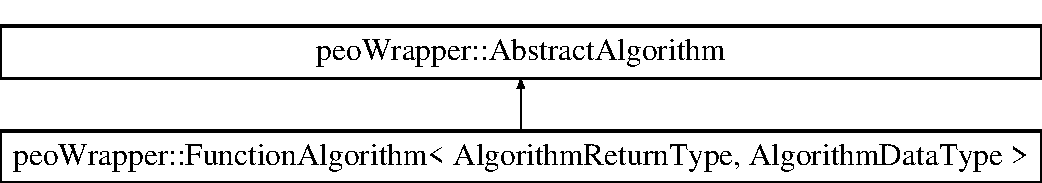
\includegraphics[height=2cm]{structpeoWrapper_1_1FunctionAlgorithm}
\end{center}
\end{figure}
\subsection*{Public Member Functions}
\begin{CompactItemize}
\item 
\hypertarget{structpeoWrapper_1_1FunctionAlgorithm_9d3994238a3f015dd0b3778ac37f7ea8}{
\hyperlink{structpeoWrapper_1_1FunctionAlgorithm_9d3994238a3f015dd0b3778ac37f7ea8}{Function\-Algorithm} (Algorithm\-Return\-Type($\ast$external\-Algorithm)(Algorithm\-Data\-Type \&), Algorithm\-Data\-Type \&external\-Data)}
\label{structpeoWrapper_1_1FunctionAlgorithm_9d3994238a3f015dd0b3778ac37f7ea8}

\item 
\hypertarget{structpeoWrapper_1_1FunctionAlgorithm_8dcef2d1fcf6147762a2809748ff6170}{
virtual void \hyperlink{structpeoWrapper_1_1FunctionAlgorithm_8dcef2d1fcf6147762a2809748ff6170}{operator()} ()}
\label{structpeoWrapper_1_1FunctionAlgorithm_8dcef2d1fcf6147762a2809748ff6170}

\end{CompactItemize}
\subsection*{Public Attributes}
\begin{CompactItemize}
\item 
\hypertarget{structpeoWrapper_1_1FunctionAlgorithm_2aef841dc81451d1585c930c7880ab09}{
Algorithm\-Data\-Type \& \hyperlink{structpeoWrapper_1_1FunctionAlgorithm_2aef841dc81451d1585c930c7880ab09}{algorithm\-Data}}
\label{structpeoWrapper_1_1FunctionAlgorithm_2aef841dc81451d1585c930c7880ab09}

\end{CompactItemize}


\subsection{Detailed Description}
\subsubsection*{template$<$typename Algorithm\-Return\-Type, typename Algorithm\-Data\-Type$>$ struct peo\-Wrapper::Function\-Algorithm$<$ Algorithm\-Return\-Type, Algorithm\-Data\-Type $>$}





Definition at line 137 of file peo\-Wrapper.h.

The documentation for this struct was generated from the following file:\begin{CompactItemize}
\item 
peo\-Wrapper.h\end{CompactItemize}

\hypertarget{structpeoWrapper_1_1FunctionAlgorithm_3_01AlgorithmReturnType_00_01void_01_4}{
\section{peo\-Wrapper::Function\-Algorithm$<$ Algorithm\-Return\-Type, void $>$ Struct Template Reference}
\label{structpeoWrapper_1_1FunctionAlgorithm_3_01AlgorithmReturnType_00_01void_01_4}\index{peoWrapper::FunctionAlgorithm< AlgorithmReturnType, void >@{peoWrapper::FunctionAlgorithm$<$ AlgorithmReturnType, void $>$}}
}
Inheritance diagram for peo\-Wrapper::Function\-Algorithm$<$ Algorithm\-Return\-Type, void $>$::\begin{figure}[H]
\begin{center}
\leavevmode
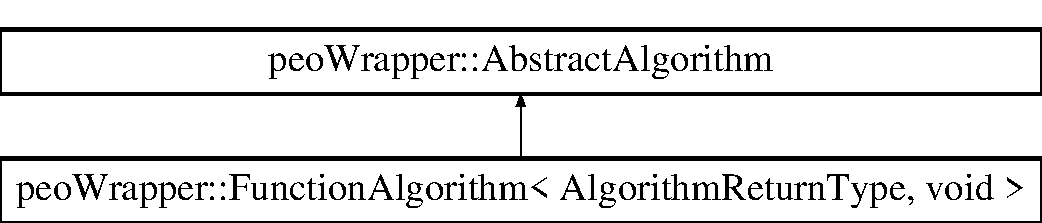
\includegraphics[height=2cm]{structpeoWrapper_1_1FunctionAlgorithm_3_01AlgorithmReturnType_00_01void_01_4}
\end{center}
\end{figure}
\subsection*{Public Member Functions}
\begin{CompactItemize}
\item 
\hypertarget{structpeoWrapper_1_1FunctionAlgorithm_3_01AlgorithmReturnType_00_01void_01_4_feb7c5fbc9915b33765ccc8e228f3d6d}{
\hyperlink{structpeoWrapper_1_1FunctionAlgorithm_3_01AlgorithmReturnType_00_01void_01_4_feb7c5fbc9915b33765ccc8e228f3d6d}{Function\-Algorithm} (Algorithm\-Return\-Type($\ast$external\-Algorithm)())}
\label{structpeoWrapper_1_1FunctionAlgorithm_3_01AlgorithmReturnType_00_01void_01_4_feb7c5fbc9915b33765ccc8e228f3d6d}

\item 
\hypertarget{structpeoWrapper_1_1FunctionAlgorithm_3_01AlgorithmReturnType_00_01void_01_4_f9803766fab40ae9dc5930b70ffbadc4}{
virtual void \hyperlink{structpeoWrapper_1_1FunctionAlgorithm_3_01AlgorithmReturnType_00_01void_01_4_f9803766fab40ae9dc5930b70ffbadc4}{operator()} ()}
\label{structpeoWrapper_1_1FunctionAlgorithm_3_01AlgorithmReturnType_00_01void_01_4_f9803766fab40ae9dc5930b70ffbadc4}

\end{CompactItemize}


\subsection{Detailed Description}
\subsubsection*{template$<$typename Algorithm\-Return\-Type$>$ struct peo\-Wrapper::Function\-Algorithm$<$ Algorithm\-Return\-Type, void $>$}





Definition at line 153 of file peo\-Wrapper.h.

The documentation for this struct was generated from the following file:\begin{CompactItemize}
\item 
peo\-Wrapper.h\end{CompactItemize}

\hypertarget{classRandomTopology}{
\section{Random\-Topology Class Reference}
\label{classRandomTopology}\index{RandomTopology@{RandomTopology}}
}
Inheritance diagram for Random\-Topology::\begin{figure}[H]
\begin{center}
\leavevmode
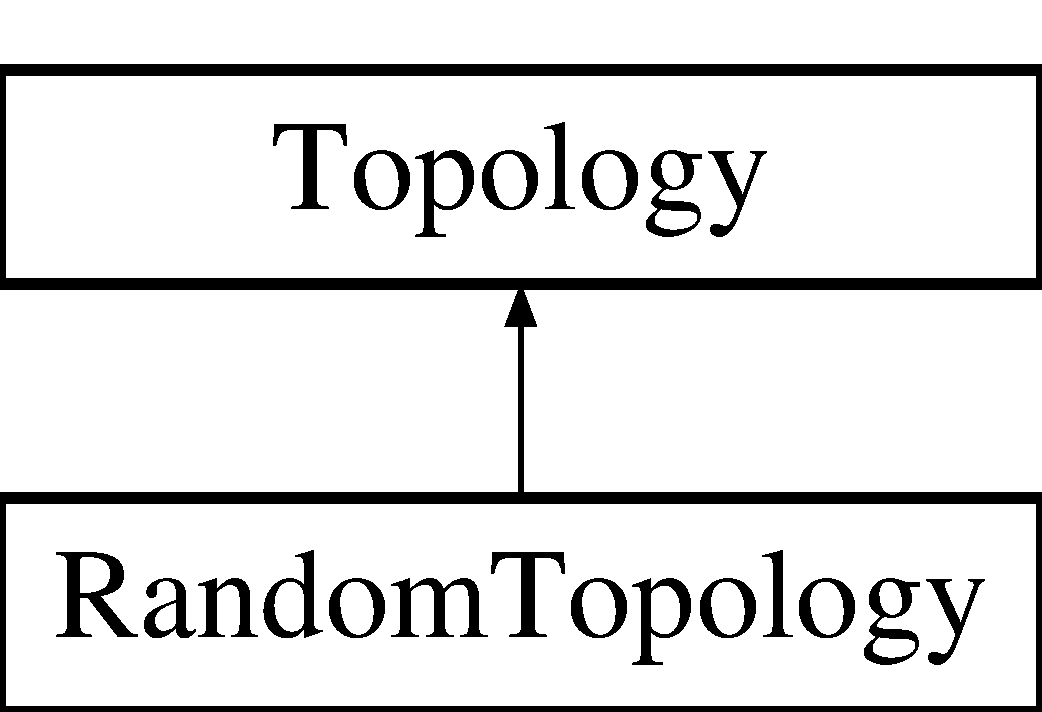
\includegraphics[height=2cm]{classRandomTopology}
\end{center}
\end{figure}
\subsection*{Public Member Functions}
\begin{CompactItemize}
\item 
\hypertarget{classRandomTopology_f68ae9feb34a8e654ab4181153803ed1}{
void \hyperlink{classRandomTopology_f68ae9feb34a8e654ab4181153803ed1}{set\-Neighbors} (\hyperlink{classCooperative}{Cooperative} $\ast$\_\-\_\-mig, std::vector$<$ \hyperlink{classCooperative}{Cooperative} $\ast$ $>$ \&\_\-\_\-from, std::vector$<$ \hyperlink{classCooperative}{Cooperative} $\ast$ $>$ \&\_\-\_\-to)}
\label{classRandomTopology_f68ae9feb34a8e654ab4181153803ed1}

\end{CompactItemize}


\subsection{Detailed Description}




Definition at line 42 of file random\_\-topo.h.

The documentation for this class was generated from the following files:\begin{CompactItemize}
\item 
random\_\-topo.h\item 
random\_\-topo.cpp\end{CompactItemize}

\hypertarget{classReactiveThread}{
\section{Reactive\-Thread Class Reference}
\label{classReactiveThread}\index{ReactiveThread@{ReactiveThread}}
}
Inheritance diagram for Reactive\-Thread::\begin{figure}[H]
\begin{center}
\leavevmode
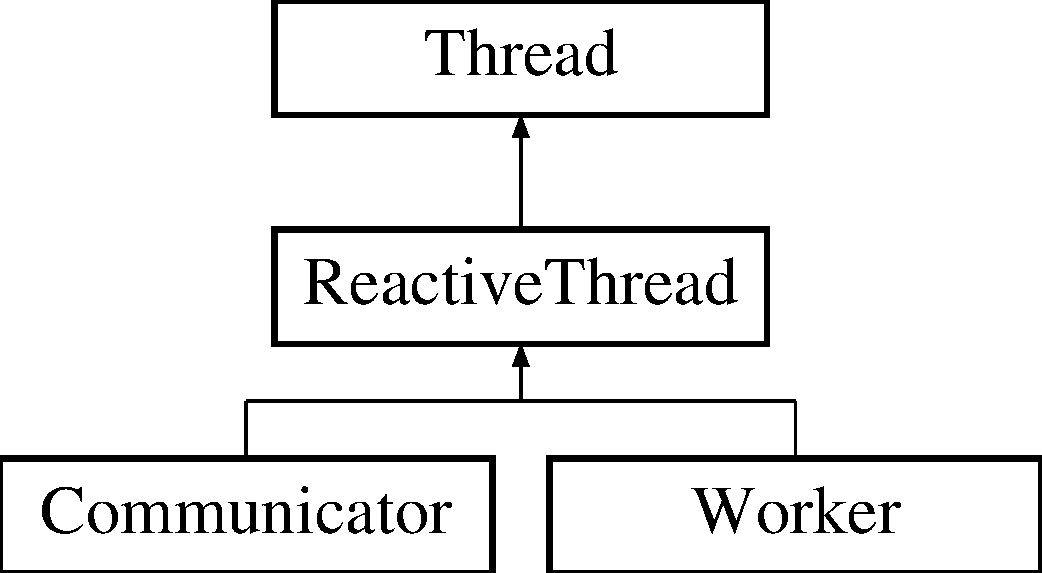
\includegraphics[height=3cm]{classReactiveThread}
\end{center}
\end{figure}
\subsection*{Public Member Functions}
\begin{CompactItemize}
\item 
\hypertarget{classReactiveThread_77381649429941c99a3e3d568113d6cf}{
\hyperlink{classReactiveThread_77381649429941c99a3e3d568113d6cf}{Reactive\-Thread} ()}
\label{classReactiveThread_77381649429941c99a3e3d568113d6cf}

\item 
\hypertarget{classReactiveThread_8263c2a32d8c99a49a05f1a7717d4262}{
void \hyperlink{classReactiveThread_8263c2a32d8c99a49a05f1a7717d4262}{sleep} ()}
\label{classReactiveThread_8263c2a32d8c99a49a05f1a7717d4262}

\item 
\hypertarget{classReactiveThread_a724a54575de10f09cc03ab7aa4e59ce}{
void \hyperlink{classReactiveThread_a724a54575de10f09cc03ab7aa4e59ce}{wake\-Up} ()}
\label{classReactiveThread_a724a54575de10f09cc03ab7aa4e59ce}

\end{CompactItemize}
\subsection*{Private Attributes}
\begin{CompactItemize}
\item 
\hypertarget{classReactiveThread_915e5a42dc8cb1bcf6738d5fe883a4e7}{
sem\_\-t \hyperlink{classReactiveThread_915e5a42dc8cb1bcf6738d5fe883a4e7}{sem}}
\label{classReactiveThread_915e5a42dc8cb1bcf6738d5fe883a4e7}

\end{CompactItemize}


\subsection{Detailed Description}




Definition at line 44 of file reac\_\-thread.h.

The documentation for this class was generated from the following files:\begin{CompactItemize}
\item 
reac\_\-thread.h\item 
reac\_\-thread.cpp\end{CompactItemize}

\hypertarget{classreplacement}{
\section{replacement$<$ TYPE $>$ Class Template Reference}
\label{classreplacement}\index{replacement@{replacement}}
}
Abstract class for a replacement within the exchange of data by migration.  


{\tt \#include $<$peo\-Data.h$>$}

Inheritance diagram for replacement$<$ TYPE $>$::\begin{figure}[H]
\begin{center}
\leavevmode
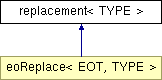
\includegraphics[height=2cm]{classreplacement}
\end{center}
\end{figure}
\subsection*{Public Member Functions}
\begin{CompactItemize}
\item 
virtual void \hyperlink{classreplacement_2c21feaad602bb9d691f0081ac4363b1}{operator()} (TYPE \&)=0
\begin{CompactList}\small\item\em Virtual operator on the template type. \item\end{CompactList}\item 
\hypertarget{classreplacement_82d1187b7f19a7bb4f251e3774f7fb88}{
virtual \hyperlink{classreplacement_82d1187b7f19a7bb4f251e3774f7fb88}{$\sim$replacement} ()}
\label{classreplacement_82d1187b7f19a7bb4f251e3774f7fb88}

\begin{CompactList}\small\item\em Virtual destructor. \item\end{CompactList}\end{CompactItemize}


\subsection{Detailed Description}
\subsubsection*{template$<$class TYPE$>$ class replacement$<$ TYPE $>$}

Abstract class for a replacement within the exchange of data by migration. 

\begin{Desc}
\item[Version:]1.0 \end{Desc}
\begin{Desc}
\item[Date:]january 2008 \end{Desc}




Definition at line 157 of file peo\-Data.h.

\subsection{Member Function Documentation}
\hypertarget{classreplacement_2c21feaad602bb9d691f0081ac4363b1}{
\index{replacement@{replacement}!operator()@{operator()}}
\index{operator()@{operator()}!replacement@{replacement}}
\subsubsection[operator()]{\setlength{\rightskip}{0pt plus 5cm}template$<$class TYPE$>$ virtual void \hyperlink{classreplacement}{replacement}$<$ TYPE $>$::operator() (TYPE \&)\hspace{0.3cm}{\tt  \mbox{[}pure virtual\mbox{]}}}}
\label{classreplacement_2c21feaad602bb9d691f0081ac4363b1}


Virtual operator on the template type. 

\begin{Desc}
\item[Parameters:]
\begin{description}
\item[{\em TYPE}]\& \end{description}
\end{Desc}


Implemented in \hyperlink{classeoReplace_786659edbd9907000138aa29caf46065}{eo\-Replace$<$ EOT, TYPE $>$}.

The documentation for this class was generated from the following file:\begin{CompactItemize}
\item 
peo\-Data.h\end{CompactItemize}

\hypertarget{classRingTopology}{
\section{Ring\-Topology Class Reference}
\label{classRingTopology}\index{RingTopology@{RingTopology}}
}
Inheritance diagram for Ring\-Topology::\begin{figure}[H]
\begin{center}
\leavevmode
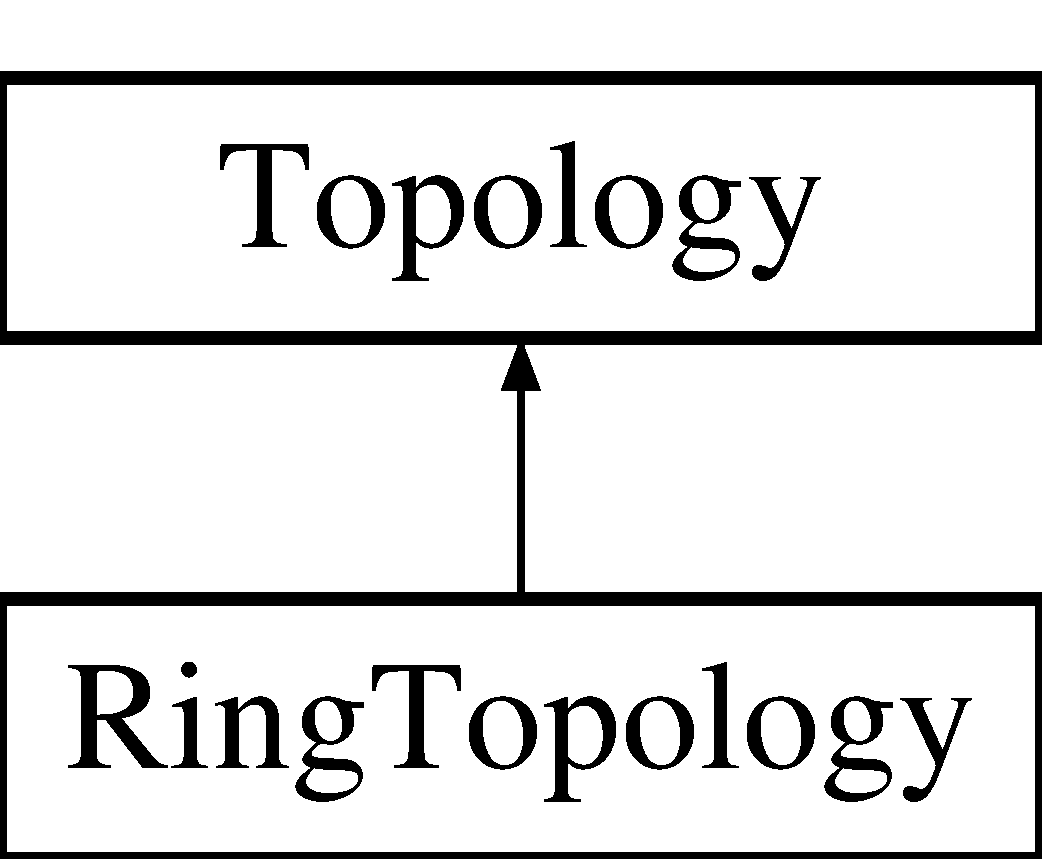
\includegraphics[height=2cm]{classRingTopology}
\end{center}
\end{figure}
\subsection*{Public Member Functions}
\begin{CompactItemize}
\item 
\hypertarget{classRingTopology_292a7746993788f96042f2f628cfcbc5}{
void \hyperlink{classRingTopology_292a7746993788f96042f2f628cfcbc5}{set\-Neighbors} (\hyperlink{classCooperative}{Cooperative} $\ast$\_\-\_\-mig, std::vector$<$ \hyperlink{classCooperative}{Cooperative} $\ast$ $>$ \&\_\-\_\-from, std::vector$<$ \hyperlink{classCooperative}{Cooperative} $\ast$ $>$ \&\_\-\_\-to)}
\label{classRingTopology_292a7746993788f96042f2f628cfcbc5}

\end{CompactItemize}


\subsection{Detailed Description}




Definition at line 42 of file ring\_\-topo.h.

The documentation for this class was generated from the following files:\begin{CompactItemize}
\item 
ring\_\-topo.h\item 
ring\_\-topo.cpp\end{CompactItemize}

\hypertarget{classRouteEval}{
\section{Route\-Eval Class Reference}
\label{classRouteEval}\index{RouteEval@{RouteEval}}
}
Inheritance diagram for Route\-Eval::\begin{figure}[H]
\begin{center}
\leavevmode
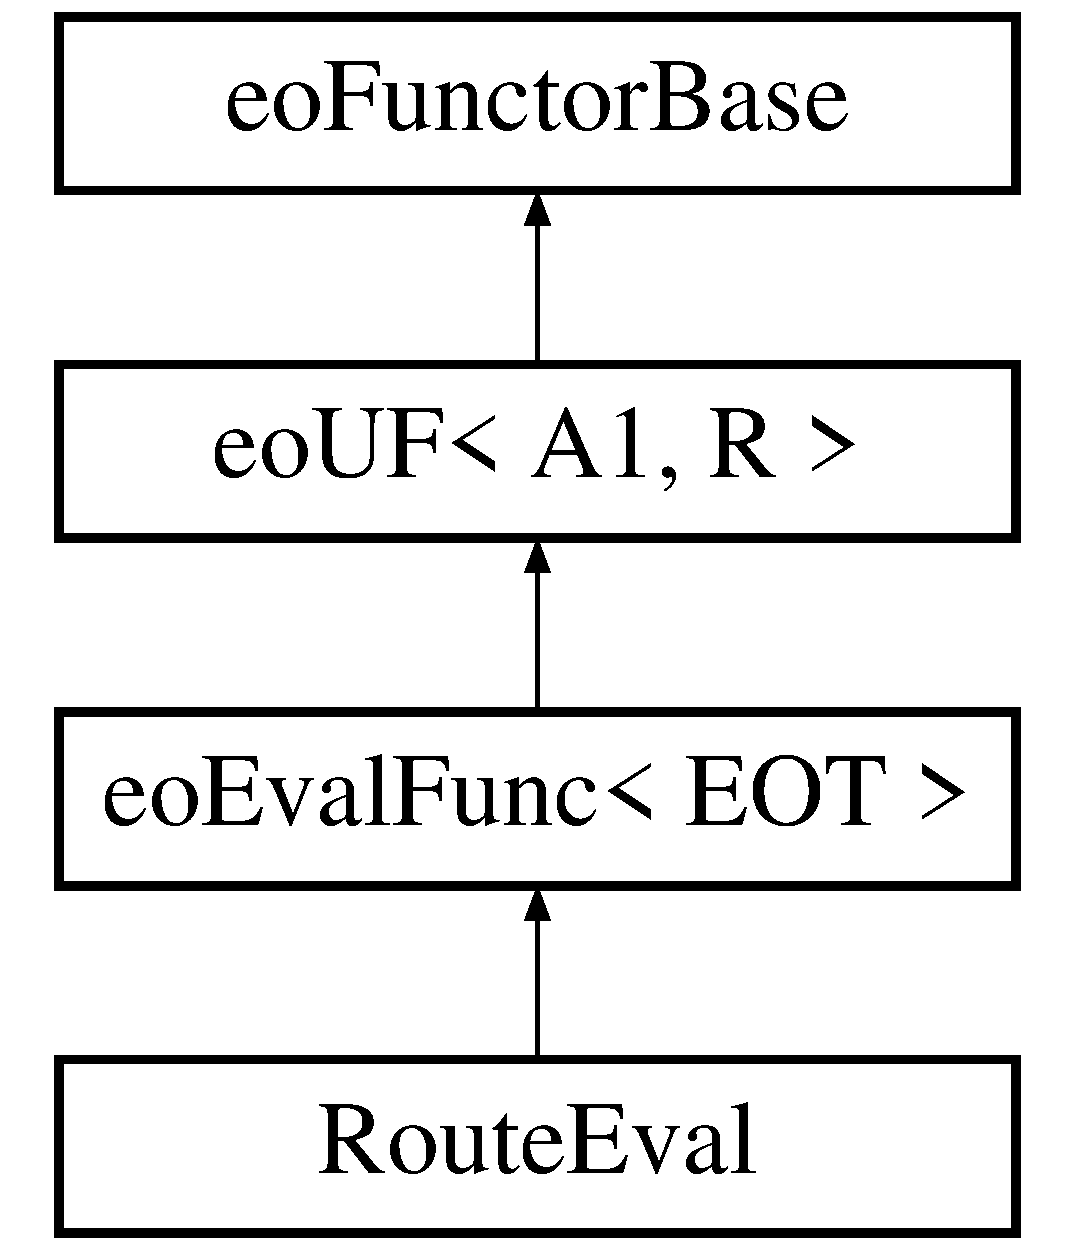
\includegraphics[height=4cm]{classRouteEval}
\end{center}
\end{figure}
\subsection*{Public Member Functions}
\begin{CompactItemize}
\item 
\hypertarget{classRouteEval_e10bbe6f792e6f44405953de4f703901}{
void \hyperlink{classRouteEval_e10bbe6f792e6f44405953de4f703901}{operator()} (\bf{Route} \&\_\-\_\-route)}
\label{classRouteEval_e10bbe6f792e6f44405953de4f703901}

\end{CompactItemize}


\subsection{Detailed Description}




Definition at line 44 of file route\_\-eval.h.

The documentation for this class was generated from the following files:\begin{CompactItemize}
\item 
route\_\-eval.h\item 
route\_\-eval.cpp\end{CompactItemize}

\hypertarget{classRouteInit}{
\section{Route\-Init Class Reference}
\label{classRouteInit}\index{RouteInit@{RouteInit}}
}
\subsection*{Public Member Functions}
\begin{CompactItemize}
\item 
\hypertarget{classRouteInit_b65a7137e114458faadb6a5510c001f7}{
void \hyperlink{classRouteInit_b65a7137e114458faadb6a5510c001f7}{operator()} (Route \&\_\-\_\-route)}
\label{classRouteInit_b65a7137e114458faadb6a5510c001f7}

\end{CompactItemize}


\subsection{Detailed Description}




Definition at line 16 of file route\_\-init.h.

The documentation for this class was generated from the following files:\begin{CompactItemize}
\item 
route\_\-init.h\item 
route\_\-init.cpp\end{CompactItemize}

\hypertarget{classRunner}{
\section{Runner Class Reference}
\label{classRunner}\index{Runner@{Runner}}
}
Inheritance diagram for Runner::\begin{figure}[H]
\begin{center}
\leavevmode
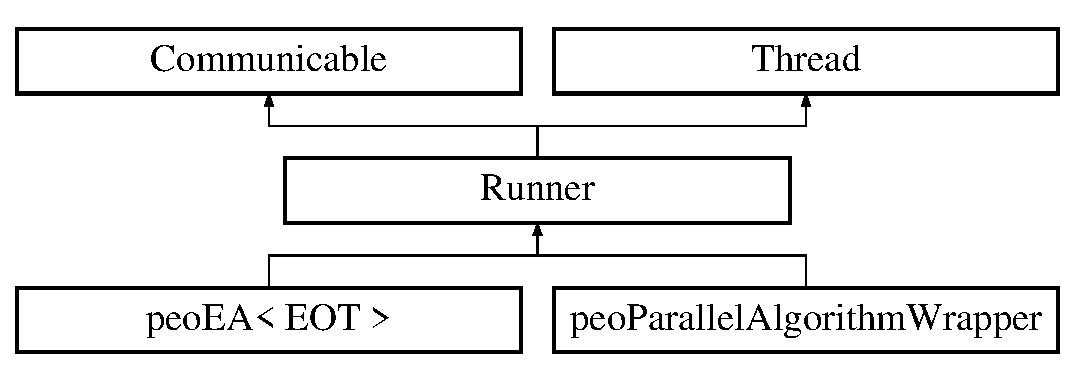
\includegraphics[height=3cm]{classRunner}
\end{center}
\end{figure}
\subsection*{Public Member Functions}
\begin{CompactItemize}
\item 
\hypertarget{classRunner_7acb8258c21da9daa62f9a177a2e5acd}{
\hyperlink{classRunner_7acb8258c21da9daa62f9a177a2e5acd}{Runner} ()}
\label{classRunner_7acb8258c21da9daa62f9a177a2e5acd}

\item 
\hypertarget{classRunner_7dc4419051fcc5cc9dadd54ecc9cd47d}{
void \hyperlink{classRunner_7dc4419051fcc5cc9dadd54ecc9cd47d}{start} ()}
\label{classRunner_7dc4419051fcc5cc9dadd54ecc9cd47d}

\item 
\hypertarget{classRunner_5bc239db2be753b77369fa9a038769fd}{
void \hyperlink{classRunner_5bc239db2be753b77369fa9a038769fd}{wait\-Starting} ()}
\label{classRunner_5bc239db2be753b77369fa9a038769fd}

\item 
\hypertarget{classRunner_40adbfb7d6944189b4fff60b02e669ca}{
bool \hyperlink{classRunner_40adbfb7d6944189b4fff60b02e669ca}{is\-Local} ()}
\label{classRunner_40adbfb7d6944189b4fff60b02e669ca}

\item 
\hypertarget{classRunner_0f133e75c28fb8264549814f80608e68}{
void \hyperlink{classRunner_0f133e75c28fb8264549814f80608e68}{terminate} ()}
\label{classRunner_0f133e75c28fb8264549814f80608e68}

\item 
\hypertarget{classRunner_5026c74eec184e3a15cb3c0ec4200a57}{
RUNNER\_\-ID \hyperlink{classRunner_5026c74eec184e3a15cb3c0ec4200a57}{get\-ID} ()}
\label{classRunner_5026c74eec184e3a15cb3c0ec4200a57}

\item 
\hypertarget{classRunner_2ad6d199d684d6f34347fc202ffe2fa3}{
void \hyperlink{classRunner_2ad6d199d684d6f34347fc202ffe2fa3}{pack\-Termination} ()}
\label{classRunner_2ad6d199d684d6f34347fc202ffe2fa3}

\item 
\hypertarget{classRunner_3591be473e0fcee1105fb57319b529aa}{
void \hyperlink{classRunner_3591be473e0fcee1105fb57319b529aa}{notify\-Sending\-Termination} ()}
\label{classRunner_3591be473e0fcee1105fb57319b529aa}

\end{CompactItemize}
\subsection*{Private Attributes}
\begin{CompactItemize}
\item 
\hypertarget{classRunner_4b0827d5df2df632db4ab71dd55e81b2}{
sem\_\-t \hyperlink{classRunner_4b0827d5df2df632db4ab71dd55e81b2}{sem\_\-start}}
\label{classRunner_4b0827d5df2df632db4ab71dd55e81b2}

\item 
\hypertarget{classRunner_1989c1f8e0b0b54ad2e60a341007e59d}{
unsigned \hyperlink{classRunner_1989c1f8e0b0b54ad2e60a341007e59d}{id}}
\label{classRunner_1989c1f8e0b0b54ad2e60a341007e59d}

\end{CompactItemize}


\subsection{Detailed Description}




Definition at line 47 of file runner.h.

The documentation for this class was generated from the following files:\begin{CompactItemize}
\item 
runner.h\item 
core/runner.cpp\item 
rmc/mpi/runner.cpp\end{CompactItemize}

\hypertarget{classselector}{
\section{selector$<$ TYPE $>$ Class Template Reference}
\label{classselector}\index{selector@{selector}}
}
Abstract class for a selector within the exchange of data by migration.  


{\tt \#include $<$peo\-Data.h$>$}

Inheritance diagram for selector$<$ TYPE $>$::\begin{figure}[H]
\begin{center}
\leavevmode
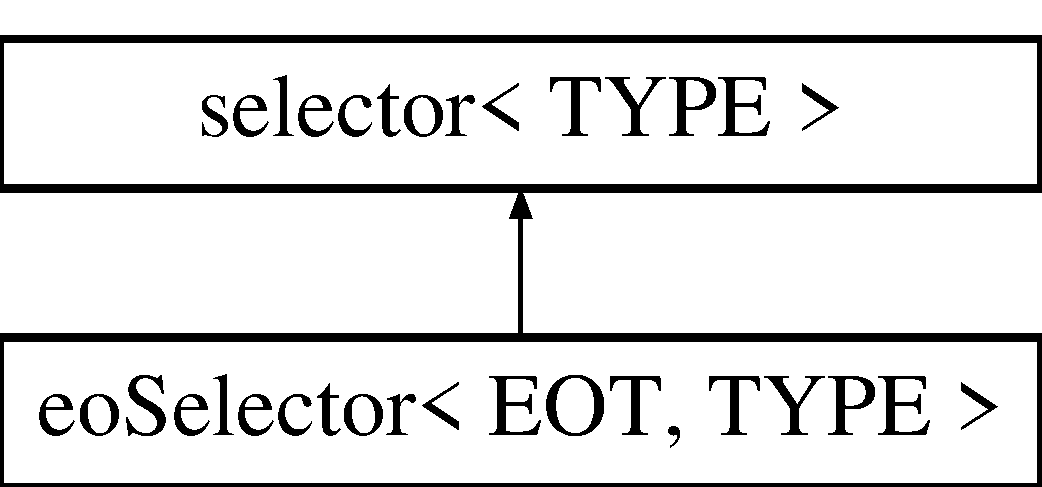
\includegraphics[height=2cm]{classselector}
\end{center}
\end{figure}
\subsection*{Public Member Functions}
\begin{CompactItemize}
\item 
virtual void \hyperlink{classselector_3ca409d57262f397263541753c7fcc28}{operator()} (TYPE \&)=0
\begin{CompactList}\small\item\em Virtual operator on the template type. \item\end{CompactList}\item 
\hypertarget{classselector_59a14168e5c0b3f5f4fcab076f4efd2b}{
virtual \hyperlink{classselector_59a14168e5c0b3f5f4fcab076f4efd2b}{$\sim$selector} ()}
\label{classselector_59a14168e5c0b3f5f4fcab076f4efd2b}

\begin{CompactList}\small\item\em Virtual destructor. \item\end{CompactList}\end{CompactItemize}


\subsection{Detailed Description}
\subsubsection*{template$<$class TYPE$>$ class selector$<$ TYPE $>$}

Abstract class for a selector within the exchange of data by migration. 

\begin{Desc}
\item[Version:]1.0 \end{Desc}
\begin{Desc}
\item[Date:]january 2008 \end{Desc}




Definition at line 101 of file peo\-Data.h.

\subsection{Member Function Documentation}
\hypertarget{classselector_3ca409d57262f397263541753c7fcc28}{
\index{selector@{selector}!operator()@{operator()}}
\index{operator()@{operator()}!selector@{selector}}
\subsubsection[operator()]{\setlength{\rightskip}{0pt plus 5cm}template$<$class TYPE$>$ virtual void \hyperlink{classselector}{selector}$<$ TYPE $>$::operator() (TYPE \&)\hspace{0.3cm}{\tt  \mbox{[}pure virtual\mbox{]}}}}
\label{classselector_3ca409d57262f397263541753c7fcc28}


Virtual operator on the template type. 

\begin{Desc}
\item[Parameters:]
\begin{description}
\item[{\em TYPE}]\& \end{description}
\end{Desc}


Implemented in \hyperlink{classeoSelector_2f32b10e23e68654e4459bb682aaa4ff}{eo\-Selector$<$ EOT, TYPE $>$}.

The documentation for this class was generated from the following file:\begin{CompactItemize}
\item 
peo\-Data.h\end{CompactItemize}

\hypertarget{structSEND__REQUEST}{
\section{SEND\_\-REQUEST Struct Reference}
\label{structSEND__REQUEST}\index{SEND_REQUEST@{SEND\_\-REQUEST}}
}
\subsection*{Public Attributes}
\begin{CompactItemize}
\item 
\hypertarget{structSEND__REQUEST_1ad8f7233fa3ff13262e783a9153920f}{
\hyperlink{classCommunicable}{Communicable} $\ast$ \hyperlink{structSEND__REQUEST_1ad8f7233fa3ff13262e783a9153920f}{comm}}
\label{structSEND__REQUEST_1ad8f7233fa3ff13262e783a9153920f}

\item 
\hypertarget{structSEND__REQUEST_93e2a6a71d2a91aa2b7bdd050ee59b4d}{
int \hyperlink{structSEND__REQUEST_93e2a6a71d2a91aa2b7bdd050ee59b4d}{to}}
\label{structSEND__REQUEST_93e2a6a71d2a91aa2b7bdd050ee59b4d}

\item 
\hypertarget{structSEND__REQUEST_3126b3ef9d6533d3086760e413a7f23f}{
int \hyperlink{structSEND__REQUEST_3126b3ef9d6533d3086760e413a7f23f}{tag}}
\label{structSEND__REQUEST_3126b3ef9d6533d3086760e413a7f23f}

\end{CompactItemize}


\subsection{Detailed Description}




Definition at line 52 of file send.cpp.

The documentation for this struct was generated from the following file:\begin{CompactItemize}
\item 
send.cpp\end{CompactItemize}

\hypertarget{classService}{
\section{Service Class Reference}
\label{classService}\index{Service@{Service}}
}
Inheritance diagram for Service::\begin{figure}[H]
\begin{center}
\leavevmode
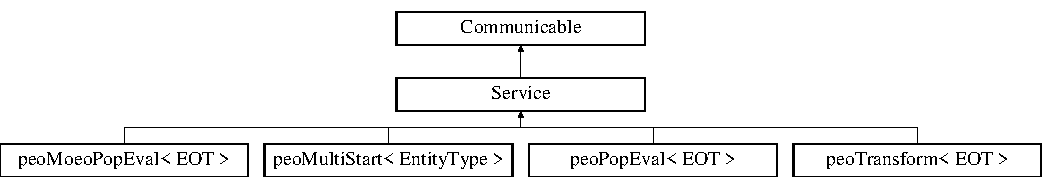
\includegraphics[height=2.8cm]{classService}
\end{center}
\end{figure}
\subsection*{Public Member Functions}
\begin{CompactItemize}
\item 
\hypertarget{classService_33b149b98498c0e7e401b0f0839d7f0d}{
void \hyperlink{classService_33b149b98498c0e7e401b0f0839d7f0d}{set\-Owner} (\hyperlink{classThread}{Thread} \&\_\-\_\-owner)}
\label{classService_33b149b98498c0e7e401b0f0839d7f0d}

\item 
\hypertarget{classService_0dae00309c51a7b7069788142aed799f}{
\hyperlink{classThread}{Thread} $\ast$ \hyperlink{classService_0dae00309c51a7b7069788142aed799f}{get\-Owner} ()}
\label{classService_0dae00309c51a7b7069788142aed799f}

\item 
\hypertarget{classService_7e2ae35a9070a05dcd46488df649896d}{
void \hyperlink{classService_7e2ae35a9070a05dcd46488df649896d}{request\-Resource\-Request} (unsigned \_\-\_\-how\_\-many=1)}
\label{classService_7e2ae35a9070a05dcd46488df649896d}

\item 
\hypertarget{classService_c4289f98d1cd9ed53e850efbb6a947bd}{
void \hyperlink{classService_c4289f98d1cd9ed53e850efbb6a947bd}{pack\-Resource\-Request} ()}
\label{classService_c4289f98d1cd9ed53e850efbb6a947bd}

\item 
\hypertarget{classService_aea4b8f7f8fb88e83862ee4bfd9ab207}{
virtual void \hyperlink{classService_aea4b8f7f8fb88e83862ee4bfd9ab207}{pack\-Data} ()}
\label{classService_aea4b8f7f8fb88e83862ee4bfd9ab207}

\item 
\hypertarget{classService_3bd87b444710813d30fd754d4d0b4df3}{
virtual void \hyperlink{classService_3bd87b444710813d30fd754d4d0b4df3}{unpack\-Data} ()}
\label{classService_3bd87b444710813d30fd754d4d0b4df3}

\item 
\hypertarget{classService_e4f2894e6121e60f38d41cfbd7447ae4}{
virtual void \hyperlink{classService_e4f2894e6121e60f38d41cfbd7447ae4}{execute} ()}
\label{classService_e4f2894e6121e60f38d41cfbd7447ae4}

\item 
\hypertarget{classService_e5e4f90b2315e15c2a2913bd370f4cf5}{
virtual void \hyperlink{classService_e5e4f90b2315e15c2a2913bd370f4cf5}{pack\-Result} ()}
\label{classService_e5e4f90b2315e15c2a2913bd370f4cf5}

\item 
\hypertarget{classService_45c06344edbfa482b91f68e2035a6099}{
virtual void \hyperlink{classService_45c06344edbfa482b91f68e2035a6099}{unpack\-Result} ()}
\label{classService_45c06344edbfa482b91f68e2035a6099}

\item 
\hypertarget{classService_81ad4d6ebb50045b8977e2ab74826f30}{
virtual void \hyperlink{classService_81ad4d6ebb50045b8977e2ab74826f30}{notify\-Sending\-Data} ()}
\label{classService_81ad4d6ebb50045b8977e2ab74826f30}

\item 
\hypertarget{classService_94e2012e76aaae3aa8199250f558d503}{
virtual void \hyperlink{classService_94e2012e76aaae3aa8199250f558d503}{notify\-Sending\-Resource\-Request} ()}
\label{classService_94e2012e76aaae3aa8199250f558d503}

\item 
\hypertarget{classService_f94cc8a5c2665d4574041737e61e9ffc}{
virtual void \hyperlink{classService_f94cc8a5c2665d4574041737e61e9ffc}{notify\-Sending\-All\-Resource\-Requests} ()}
\label{classService_f94cc8a5c2665d4574041737e61e9ffc}

\end{CompactItemize}
\subsection*{Private Attributes}
\begin{CompactItemize}
\item 
\hypertarget{classService_8b615c65c876f342fe8209eb7e36d7b2}{
\hyperlink{classThread}{Thread} $\ast$ \hyperlink{classService_8b615c65c876f342fe8209eb7e36d7b2}{owner}}
\label{classService_8b615c65c876f342fe8209eb7e36d7b2}

\item 
\hypertarget{classService_a5b2ad9520bb3710b54348b99acebd58}{
unsigned \hyperlink{classService_a5b2ad9520bb3710b54348b99acebd58}{num\_\-sent\_\-rr}}
\label{classService_a5b2ad9520bb3710b54348b99acebd58}

\end{CompactItemize}


\subsection{Detailed Description}




Definition at line 17 of file service.h.

The documentation for this class was generated from the following files:\begin{CompactItemize}
\item 
service.h\item 
core/service.cpp\item 
rmc/mpi/service.cpp\end{CompactItemize}

\hypertarget{classStarTopology}{
\section{Star\-Topology Class Reference}
\label{classStarTopology}\index{StarTopology@{StarTopology}}
}
Inheritance diagram for Star\-Topology::\begin{figure}[H]
\begin{center}
\leavevmode
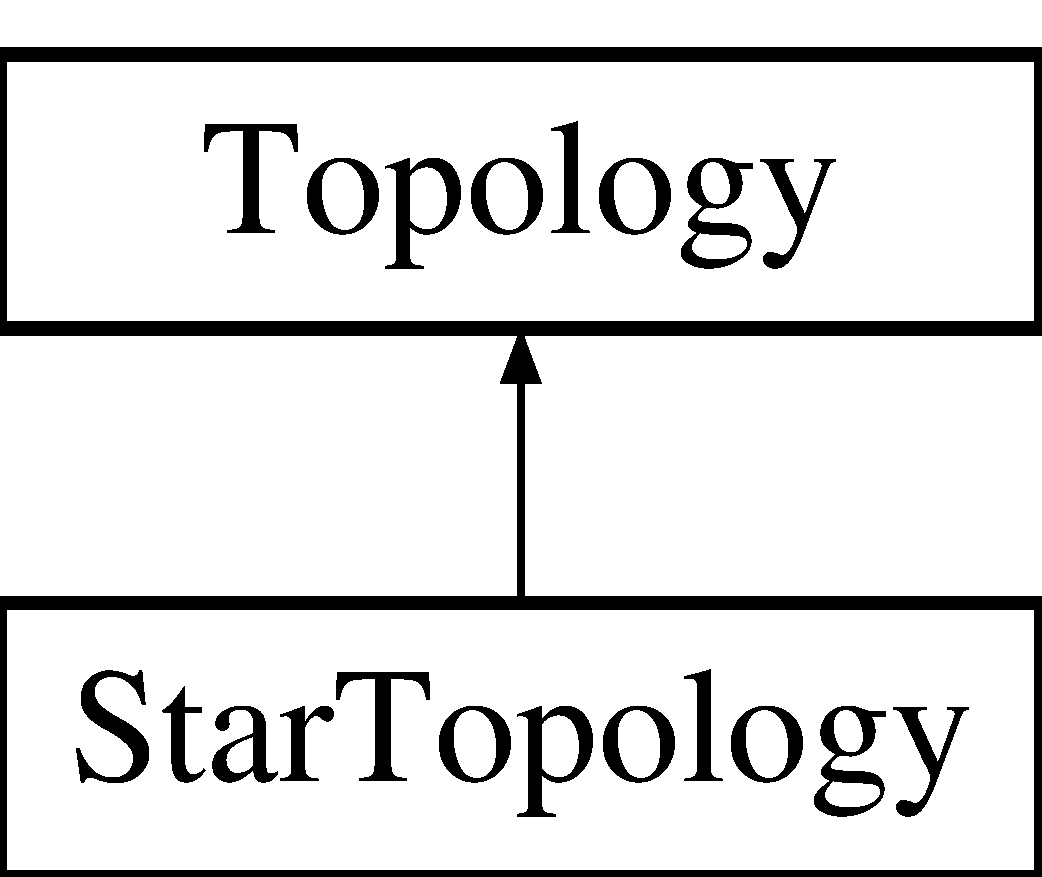
\includegraphics[height=2cm]{classStarTopology}
\end{center}
\end{figure}
\subsection*{Public Member Functions}
\begin{CompactItemize}
\item 
\hypertarget{classStarTopology_76868b70acc93be7c53a57678674b833}{
\hyperlink{classStarTopology_76868b70acc93be7c53a57678674b833}{Star\-Topology} ()}
\label{classStarTopology_76868b70acc93be7c53a57678674b833}

\item 
\hypertarget{classStarTopology_e9e129ce442849474d660add8fd96993}{
void \hyperlink{classStarTopology_e9e129ce442849474d660add8fd96993}{set\-Neighbors} (\hyperlink{classCooperative}{Cooperative} $\ast$\_\-\_\-mig, std::vector$<$ \hyperlink{classCooperative}{Cooperative} $\ast$ $>$ \&\_\-\_\-from, std::vector$<$ \hyperlink{classCooperative}{Cooperative} $\ast$ $>$ \&\_\-\_\-to)}
\label{classStarTopology_e9e129ce442849474d660add8fd96993}

\item 
\hypertarget{classStarTopology_a7d8dfebd83b70cd1962b475fd0f5d8d}{
void \hyperlink{classStarTopology_a7d8dfebd83b70cd1962b475fd0f5d8d}{set\-Center} (\hyperlink{classCooperative}{Cooperative} \&\_\-\_\-center)}
\label{classStarTopology_a7d8dfebd83b70cd1962b475fd0f5d8d}

\end{CompactItemize}
\subsection*{Private Attributes}
\begin{CompactItemize}
\item 
\hypertarget{classStarTopology_5cc9978f2a1307ad0164ba129297d305}{
\hyperlink{classCooperative}{Cooperative} $\ast$ \hyperlink{classStarTopology_5cc9978f2a1307ad0164ba129297d305}{center}}
\label{classStarTopology_5cc9978f2a1307ad0164ba129297d305}

\end{CompactItemize}


\subsection{Detailed Description}




Definition at line 42 of file star\_\-topo.h.

The documentation for this class was generated from the following files:\begin{CompactItemize}
\item 
star\_\-topo.h\item 
star\_\-topo.cpp\end{CompactItemize}

\hypertarget{structSyncCompare}{
\section{Sync\-Compare Struct Reference}
\label{structSyncCompare}\index{SyncCompare@{SyncCompare}}
}
\subsection*{Public Member Functions}
\begin{CompactItemize}
\item 
\hypertarget{structSyncCompare_26ba03de10f15ad5e3fcb81c2a4244c0}{
bool \hyperlink{structSyncCompare_26ba03de10f15ad5e3fcb81c2a4244c0}{operator()} (const std::pair$<$ std::vector$<$ \hyperlink{structSyncEntry}{Sync\-Entry} $>$, unsigned $>$ \&A, const std::pair$<$ std::vector$<$ \hyperlink{structSyncEntry}{Sync\-Entry} $>$, unsigned $>$ \&B)}
\label{structSyncCompare_26ba03de10f15ad5e3fcb81c2a4244c0}

\end{CompactItemize}


\subsection{Detailed Description}




Definition at line 54 of file synchron.h.

The documentation for this struct was generated from the following file:\begin{CompactItemize}
\item 
synchron.h\end{CompactItemize}

\hypertarget{structSyncEntry}{
\section{Sync\-Entry Struct Reference}
\label{structSyncEntry}\index{SyncEntry@{SyncEntry}}
}
\subsection*{Public Attributes}
\begin{CompactItemize}
\item 
\hypertarget{structSyncEntry_4a41a06c6c4325831c08d086812d6374}{
RUNNER\_\-ID \hyperlink{structSyncEntry_4a41a06c6c4325831c08d086812d6374}{runner}}
\label{structSyncEntry_4a41a06c6c4325831c08d086812d6374}

\item 
\hypertarget{structSyncEntry_145d9df059f130c90766acf6635dba3b}{
COOP\_\-ID \hyperlink{structSyncEntry_145d9df059f130c90766acf6635dba3b}{coop}}
\label{structSyncEntry_145d9df059f130c90766acf6635dba3b}

\end{CompactItemize}


\subsection{Detailed Description}




Definition at line 47 of file synchron.h.

The documentation for this struct was generated from the following file:\begin{CompactItemize}
\item 
synchron.h\end{CompactItemize}

\hypertarget{classThread}{
\section{Thread Class Reference}
\label{classThread}\index{Thread@{Thread}}
}
Inheritance diagram for Thread::\begin{figure}[H]
\begin{center}
\leavevmode
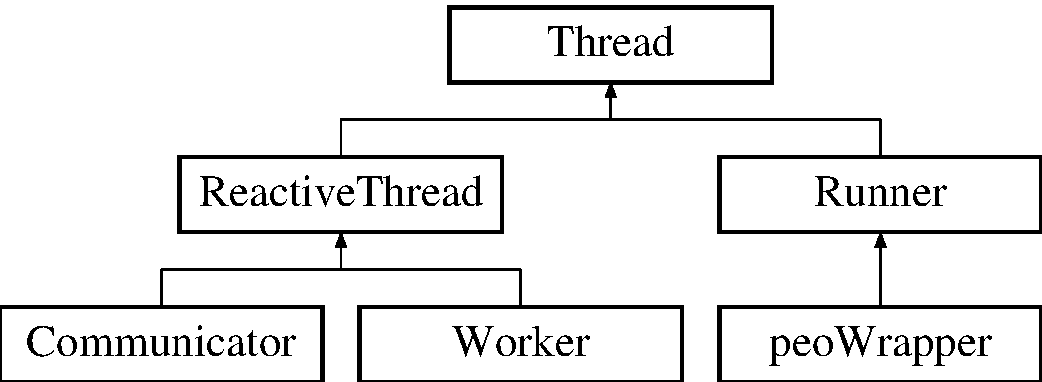
\includegraphics[height=3cm]{classThread}
\end{center}
\end{figure}
\subsection*{Public Member Functions}
\begin{CompactItemize}
\item 
\hypertarget{classThread_95c703fb8f2f27cb64f475a8c940864a}{
\hyperlink{classThread_95c703fb8f2f27cb64f475a8c940864a}{Thread} ()}
\label{classThread_95c703fb8f2f27cb64f475a8c940864a}

\item 
\hypertarget{classThread_37d9edd3a1a776cbc27dedff949c9726}{
virtual \hyperlink{classThread_37d9edd3a1a776cbc27dedff949c9726}{$\sim$Thread} ()}
\label{classThread_37d9edd3a1a776cbc27dedff949c9726}

\item 
\hypertarget{classThread_e197c46f8f62ecce6d2a7fe95bdc5b38}{
void \hyperlink{classThread_e197c46f8f62ecce6d2a7fe95bdc5b38}{set\-Active} ()}
\label{classThread_e197c46f8f62ecce6d2a7fe95bdc5b38}

\item 
\hypertarget{classThread_20632ffe9ddfa2a478afb0c84dc1096b}{
void \hyperlink{classThread_20632ffe9ddfa2a478afb0c84dc1096b}{set\-Passive} ()}
\label{classThread_20632ffe9ddfa2a478afb0c84dc1096b}

\end{CompactItemize}
\subsection*{Private Attributes}
\begin{CompactItemize}
\item 
\hypertarget{classThread_1b155d63bca3096ac4a1d039aea83c7c}{
bool \hyperlink{classThread_1b155d63bca3096ac4a1d039aea83c7c}{act}}
\label{classThread_1b155d63bca3096ac4a1d039aea83c7c}

\end{CompactItemize}


\subsection{Detailed Description}




Definition at line 31 of file thread.h.

The documentation for this class was generated from the following files:\begin{CompactItemize}
\item 
thread.h\item 
thread.cpp\end{CompactItemize}

\hypertarget{classTopology}{
\section{Topology Class Reference}
\label{classTopology}\index{Topology@{Topology}}
}
Inheritance diagram for Topology::\begin{figure}[H]
\begin{center}
\leavevmode
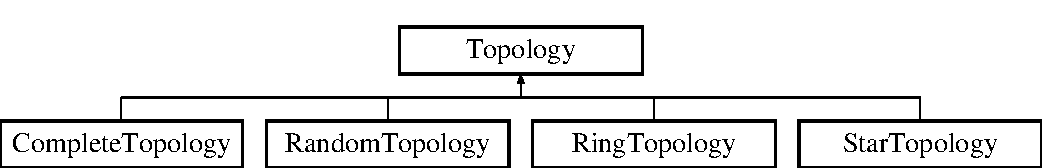
\includegraphics[height=2cm]{classTopology}
\end{center}
\end{figure}
\subsection*{Public Member Functions}
\begin{CompactItemize}
\item 
\hypertarget{classTopology_3e447669757c8311c7f6f8edc705abf2}{
virtual \hyperlink{classTopology_3e447669757c8311c7f6f8edc705abf2}{$\sim$Topology} ()}
\label{classTopology_3e447669757c8311c7f6f8edc705abf2}

\item 
\hypertarget{classTopology_62bc46d8c20fdc71dad9e7c7a0d7aded}{
void \hyperlink{classTopology_62bc46d8c20fdc71dad9e7c7a0d7aded}{add} (\hyperlink{classCooperative}{Cooperative} \&\_\-\_\-mig)}
\label{classTopology_62bc46d8c20fdc71dad9e7c7a0d7aded}

\end{CompactItemize}
\subsection*{Protected Attributes}
\begin{CompactItemize}
\item 
\hypertarget{classTopology_247a2faa8568b678f0b7b11e62c7812c}{
std::vector$<$ \hyperlink{classCooperative}{Cooperative} $\ast$ $>$ \hyperlink{classTopology_247a2faa8568b678f0b7b11e62c7812c}{mig}}
\label{classTopology_247a2faa8568b678f0b7b11e62c7812c}

\end{CompactItemize}


\subsection{Detailed Description}




Definition at line 16 of file topology.h.

The documentation for this class was generated from the following files:\begin{CompactItemize}
\item 
topology.h\item 
topology.cpp\end{CompactItemize}

\hypertarget{classTwoOpt}{
\section{Two\-Opt Class Reference}
\label{classTwoOpt}\index{TwoOpt@{TwoOpt}}
}
Inheritance diagram for Two\-Opt::\begin{figure}[H]
\begin{center}
\leavevmode
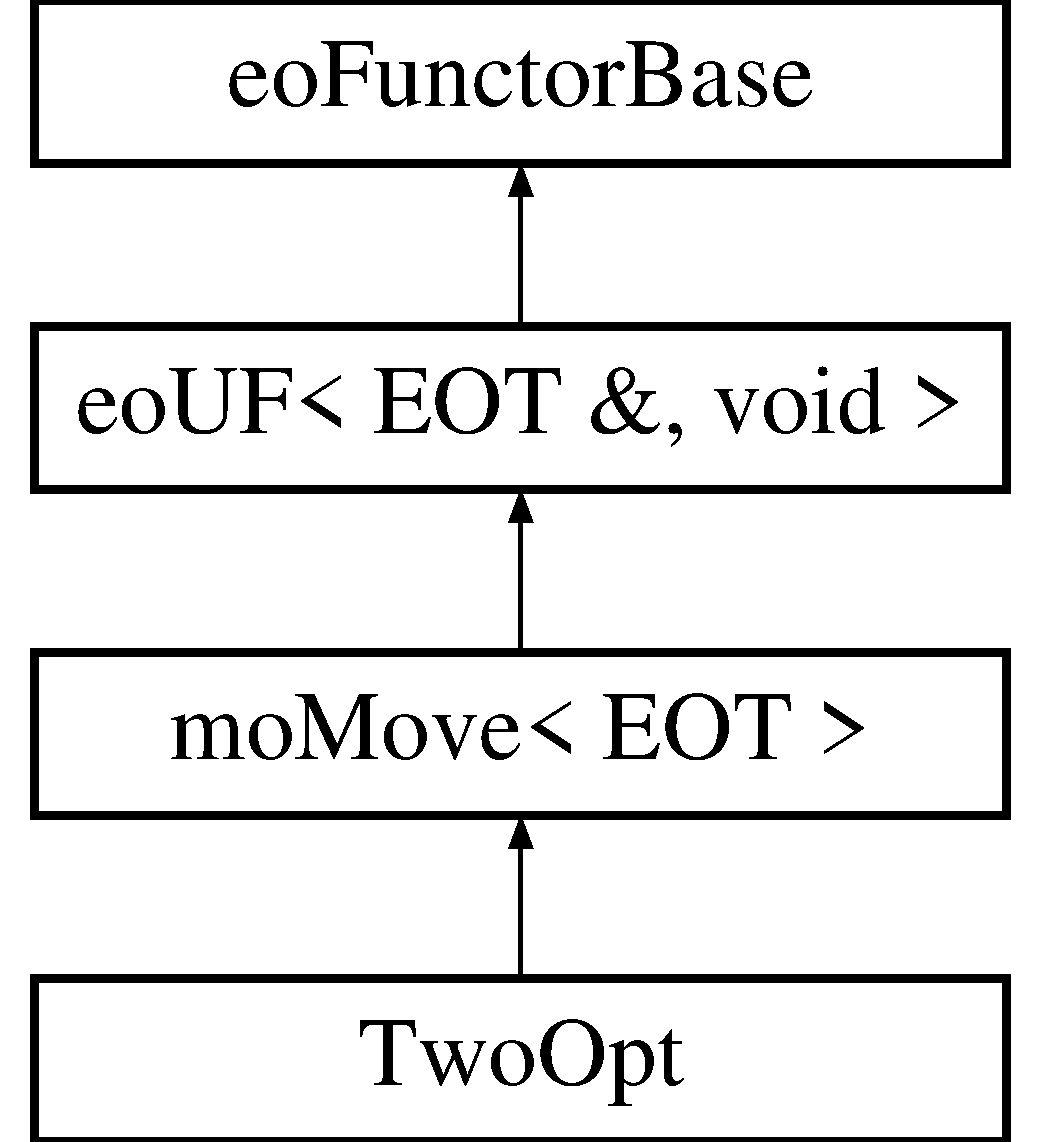
\includegraphics[height=2cm]{classTwoOpt}
\end{center}
\end{figure}
\subsection*{Public Member Functions}
\begin{CompactItemize}
\item 
\hypertarget{classTwoOpt_ff87d1649a33d42a6d64e8d314ed1af0}{
void \hyperlink{classTwoOpt_ff87d1649a33d42a6d64e8d314ed1af0}{operator()} (Route \&\_\-\_\-route)}
\label{classTwoOpt_ff87d1649a33d42a6d64e8d314ed1af0}

\end{CompactItemize}


\subsection{Detailed Description}




Definition at line 17 of file two\_\-opt.h.

The documentation for this class was generated from the following files:\begin{CompactItemize}
\item 
two\_\-opt.h\item 
two\_\-opt.cpp\end{CompactItemize}

\hypertarget{classTwoOptIncrEval}{
\section{Two\-Opt\-Incr\-Eval Class Reference}
\label{classTwoOptIncrEval}\index{TwoOptIncrEval@{TwoOptIncrEval}}
}
\subsection*{Public Member Functions}
\begin{CompactItemize}
\item 
\hypertarget{classTwoOptIncrEval_48500077e651c4c6152daef8a396be39}{
int \hyperlink{classTwoOptIncrEval_48500077e651c4c6152daef8a396be39}{operator()} (const \hyperlink{classTwoOpt}{Two\-Opt} \&\_\-\_\-move, const Route \&\_\-\_\-route)}
\label{classTwoOptIncrEval_48500077e651c4c6152daef8a396be39}

\end{CompactItemize}


\subsection{Detailed Description}




Definition at line 30 of file two\_\-opt\_\-incr\_\-eval.h.

The documentation for this class was generated from the following files:\begin{CompactItemize}
\item 
two\_\-opt\_\-incr\_\-eval.h\item 
two\_\-opt\_\-incr\_\-eval.cpp\end{CompactItemize}

\hypertarget{classTwoOptInit}{
\section{Two\-Opt\-Init Class Reference}
\label{classTwoOptInit}\index{TwoOptInit@{TwoOptInit}}
}
Inheritance diagram for Two\-Opt\-Init::\begin{figure}[H]
\begin{center}
\leavevmode
\includegraphics[height=4cm]{classTwoOptInit}
\end{center}
\end{figure}
\subsection*{Public Member Functions}
\begin{CompactItemize}
\item 
\hypertarget{classTwoOptInit_5bf6af064d37ebd955ffb5a623e78e1b}{
void \hyperlink{classTwoOptInit_5bf6af064d37ebd955ffb5a623e78e1b}{operator()} (\hyperlink{classTwoOpt}{Two\-Opt} \&\_\-\_\-move, const \bf{Route} \&\_\-\_\-route)}
\label{classTwoOptInit_5bf6af064d37ebd955ffb5a623e78e1b}

\end{CompactItemize}


\subsection{Detailed Description}




Definition at line 44 of file two\_\-opt\_\-init.h.

The documentation for this class was generated from the following files:\begin{CompactItemize}
\item 
two\_\-opt\_\-init.h\item 
two\_\-opt\_\-init.cpp\end{CompactItemize}

\hypertarget{classTwoOptNext}{
\section{Two\-Opt\-Next Class Reference}
\label{classTwoOptNext}\index{TwoOptNext@{TwoOptNext}}
}
Inheritance diagram for Two\-Opt\-Next::\begin{figure}[H]
\begin{center}
\leavevmode
\includegraphics[height=4cm]{classTwoOptNext}
\end{center}
\end{figure}
\subsection*{Public Member Functions}
\begin{CompactItemize}
\item 
\hypertarget{classTwoOptNext_baf229b2e056f39ab971cf2ac66a833e}{
bool \hyperlink{classTwoOptNext_baf229b2e056f39ab971cf2ac66a833e}{operator()} (\hyperlink{classTwoOpt}{Two\-Opt} \&\_\-\_\-move, const \bf{Route} \&\_\-\_\-route)}
\label{classTwoOptNext_baf229b2e056f39ab971cf2ac66a833e}

\end{CompactItemize}


\subsection{Detailed Description}




Definition at line 44 of file two\_\-opt\_\-next.h.

The documentation for this class was generated from the following files:\begin{CompactItemize}
\item 
two\_\-opt\_\-next.h\item 
two\_\-opt\_\-next.cpp\end{CompactItemize}

\hypertarget{classTwoOptRand}{
\section{Two\-Opt\-Rand Class Reference}
\label{classTwoOptRand}\index{TwoOptRand@{TwoOptRand}}
}
\subsection*{Public Member Functions}
\begin{CompactItemize}
\item 
\hypertarget{classTwoOptRand_e2f362f359517c027f6f22fba0aab375}{
void \hyperlink{classTwoOptRand_e2f362f359517c027f6f22fba0aab375}{operator()} (\hyperlink{classTwoOpt}{Two\-Opt} \&\_\-\_\-move, const Route \&\_\-\_\-route)}
\label{classTwoOptRand_e2f362f359517c027f6f22fba0aab375}

\end{CompactItemize}


\subsection{Detailed Description}




Definition at line 16 of file two\_\-opt\_\-rand.h.

The documentation for this class was generated from the following files:\begin{CompactItemize}
\item 
two\_\-opt\_\-rand.h\item 
two\_\-opt\_\-rand.cpp\end{CompactItemize}

\hypertarget{classWorker}{
\section{Worker Class Reference}
\label{classWorker}\index{Worker@{Worker}}
}
Inheritance diagram for Worker::\begin{figure}[H]
\begin{center}
\leavevmode
\includegraphics[height=3cm]{classWorker}
\end{center}
\end{figure}
\subsection*{Public Member Functions}
\begin{CompactItemize}
\item 
\hypertarget{classWorker_3754817df06ffe220f7f0d903c78ccac}{
\hyperlink{classWorker_3754817df06ffe220f7f0d903c78ccac}{Worker} ()}
\label{classWorker_3754817df06ffe220f7f0d903c78ccac}

\item 
\hypertarget{classWorker_abcbbace05c6113f1959c494b3577291}{
void \hyperlink{classWorker_abcbbace05c6113f1959c494b3577291}{start} ()}
\label{classWorker_abcbbace05c6113f1959c494b3577291}

\item 
\hypertarget{classWorker_83780920118e6c2b67d9477bdf8be248}{
void \hyperlink{classWorker_83780920118e6c2b67d9477bdf8be248}{pack\-Result} ()}
\label{classWorker_83780920118e6c2b67d9477bdf8be248}

\item 
\hypertarget{classWorker_bff2bdcd64fe5400156cc78704c64953}{
void \hyperlink{classWorker_bff2bdcd64fe5400156cc78704c64953}{unpack\-Data} ()}
\label{classWorker_bff2bdcd64fe5400156cc78704c64953}

\item 
\hypertarget{classWorker_60d2e8eba85b9ef403d94be54c391640}{
void \hyperlink{classWorker_60d2e8eba85b9ef403d94be54c391640}{pack\-Task\-Done} ()}
\label{classWorker_60d2e8eba85b9ef403d94be54c391640}

\item 
\hypertarget{classWorker_e2f487014766a73c5788bdcfd58ad863}{
void \hyperlink{classWorker_e2f487014766a73c5788bdcfd58ad863}{notify\-Sending\-Result} ()}
\label{classWorker_e2f487014766a73c5788bdcfd58ad863}

\item 
\hypertarget{classWorker_13efd6a8e275745329a4a8e23a0eb0bb}{
void \hyperlink{classWorker_13efd6a8e275745329a4a8e23a0eb0bb}{notify\-Sending\-Task\-Done} ()}
\label{classWorker_13efd6a8e275745329a4a8e23a0eb0bb}

\item 
\hypertarget{classWorker_5dab4ea663546b5a49d9398d7a624d27}{
void \hyperlink{classWorker_5dab4ea663546b5a49d9398d7a624d27}{set\-Source} (int \_\-\_\-rank)}
\label{classWorker_5dab4ea663546b5a49d9398d7a624d27}

\end{CompactItemize}
\subsection*{Private Attributes}
\begin{CompactItemize}
\item 
\hypertarget{classWorker_b5ffcb995e12fa71b9551e91729d6972}{
WORKER\_\-ID \hyperlink{classWorker_b5ffcb995e12fa71b9551e91729d6972}{id}}
\label{classWorker_b5ffcb995e12fa71b9551e91729d6972}

\item 
\hypertarget{classWorker_d7dc76e301fd2bcf5d3a2088a59f1378}{
SERVICE\_\-ID \hyperlink{classWorker_d7dc76e301fd2bcf5d3a2088a59f1378}{serv\_\-id}}
\label{classWorker_d7dc76e301fd2bcf5d3a2088a59f1378}

\item 
\hypertarget{classWorker_454e1764ed165af733cc44a73e395692}{
\hyperlink{classService}{Service} $\ast$ \hyperlink{classWorker_454e1764ed165af733cc44a73e395692}{serv}}
\label{classWorker_454e1764ed165af733cc44a73e395692}

\item 
\hypertarget{classWorker_895c3ebc198018ea3391c09bc802d2f6}{
int \hyperlink{classWorker_895c3ebc198018ea3391c09bc802d2f6}{src}}
\label{classWorker_895c3ebc198018ea3391c09bc802d2f6}

\item 
\hypertarget{classWorker_7ba5a18b2918cf9e704536b763be37f7}{
bool \hyperlink{classWorker_7ba5a18b2918cf9e704536b763be37f7}{toto}}
\label{classWorker_7ba5a18b2918cf9e704536b763be37f7}

\end{CompactItemize}


\subsection{Detailed Description}




Definition at line 33 of file worker.h.

The documentation for this class was generated from the following files:\begin{CompactItemize}
\item 
worker.h\item 
worker.cpp\end{CompactItemize}

\printindex
\end{document}
